%% LyX 2.3.7 created this file.  For more info, see http://www.lyx.org/.
%% Do not edit unless you really know what you are doing.
\documentclass[journal,article,submit,pdftex,moreauthors]{Definitions/mdpi}
\usepackage[utf8]{inputenc}
\usepackage{float}
\usepackage{textcomp}
\usepackage{url}
\usepackage{graphicx}

\makeatletter

%%%%%%%%%%%%%%%%%%%%%%%%%%%%%% LyX specific LaTeX commands.

\Title{Neural DE: an evolutionary method based on Differential Evolution
suitable for neural network training}

\TitleCitation{Neural DE: an evolutionary method based on Differential Evolution
suitable for neural network training}

\Author{Ioannis G. Tsoulos$^{1,*}$, Vasileios Charilogis$^{2}$}

\AuthorNames{Ioannis G. Tsoulos; Vasileios Charilogis}

\AuthorCitation{Tsoulos, I.G.; Charilogis V.}


\address{$^{1}$\quad{}Department of Informatics and Telecommunications,
University of Ioannina, Greece;itsoulos@uoi.gr\\
$^{2}\quad$Department of Informatics and Telecommunications, University
of Ioannina, Greece; v.charilog@uoi.gr}


\corres{Correspondence: itsoulos@uoi.gr; }


\abstract{Artificial neural networks have proven to be an important machine
learning model that has been widely used in recent decades in a number
of difficult problems of classification or data fitting from real
- world areas. Due to their importance, a number of techniques have
been developed that efficiently identify the parameter vector for
these models. These techniques usually come from the field of optimization
and, by minimizing the training error of artificial neural networks,
estimate the vector of their parameters. However, many times these
techniques either get trapped in local minima of the training error
or lead to overfitting the artificial neural network, resulting in
poor performance when applied to data that was not present during
the training process. This paper presents an innovative training technique
for artificial neural networks based on the Differential Evolution
optimization method. This new technique creates an initial population
of artificial neural networks that evolve and periodically applies
a local optimization technique in order to accelerate the training
of these networks. The application of the local minimization technique
is done in such a way as to avoid the phenomenon of overfitting. This
new method was successfully applied to a series of classification
and data fitting problems and a comparative study was made with other
training techniques from the relevant literature.}


\keyword{Neural networks; Evolutionary methods; Differential Evolution; Machine
learning}

\DeclareTextSymbolDefault{\textquotedbl}{T1}
%% Because html converters don't know tabularnewline
\providecommand{\tabularnewline}{\\}

%%%%%%%%%%%%%%%%%%%%%%%%%%%%%% User specified LaTeX commands.
%  LaTeX support: latex@mdpi.com 
%  For support, please attach all files needed for compiling as well as the log file, and specify your operating system, LaTeX version, and LaTeX editor.

%=================================================================


% For posting an early version of this manuscript as a preprint, you may use "preprints" as the journal and change "submit" to "accept". The document class line would be, e.g., \documentclass[preprints,article,accept,moreauthors,pdftex]{mdpi}. This is especially recommended for submission to arXiv, where line numbers should be removed before posting. For preprints.org, the editorial staff will make this change immediately prior to posting.

%--------------------
% Class Options:
%--------------------
%----------
% journal
%----------
% Choose between the following MDPI journals:
% acoustics, actuators, addictions, admsci, adolescents, aerospace, agriculture, agriengineering, agronomy, ai, algorithms, allergies, alloys, analytica, animals, antibiotics, antibodies, antioxidants, applbiosci, appliedchem, appliedmath, applmech, applmicrobiol, applnano, applsci, aquacj, architecture, arts, asc, asi, astronomy, atmosphere, atoms, audiolres, automation, axioms, bacteria, batteries, bdcc, behavsci, beverages, biochem, bioengineering, biologics, biology, biomass, biomechanics, biomed, biomedicines, biomedinformatics, biomimetics, biomolecules, biophysica, biosensors, biotech, birds, bloods, blsf, brainsci, breath, buildings, businesses, cancers, carbon, cardiogenetics, catalysts, cells, ceramics, challenges, chemengineering, chemistry, chemosensors, chemproc, children, chips, cimb, civileng, cleantechnol, climate, clinpract, clockssleep, cmd, coasts, coatings, colloids, colorants, commodities, compounds, computation, computers, condensedmatter, conservation, constrmater, cosmetics, covid, crops, cryptography, crystals, csmf, ctn, curroncol, currophthalmol, cyber, dairy, data, dentistry, dermato, dermatopathology, designs, diabetology, diagnostics, dietetics, digital, disabilities, diseases, diversity, dna, drones, dynamics, earth, ebj, ecologies, econometrics, economies, education, ejihpe, electricity, electrochem, electronicmat, electronics, encyclopedia, endocrines, energies, eng, engproc, ent, entomology, entropy, environments, environsciproc, epidemiologia, epigenomes, est, fermentation, fibers, fintech, fire, fishes, fluids, foods, forecasting, forensicsci, forests, foundations, fractalfract, fuels, futureinternet, futureparasites, futurepharmacol, futurephys, futuretransp, galaxies, games, gases, gastroent, gastrointestdisord, gels, genealogy, genes, geographies, geohazards, geomatics, geosciences, geotechnics, geriatrics, hazardousmatters, healthcare, hearts, hemato, heritage, highthroughput, histories, horticulturae, humanities, humans, hydrobiology, hydrogen, hydrology, hygiene, idr, ijerph, ijfs, ijgi, ijms, ijns, ijtm, ijtpp, immuno, informatics, information, infrastructures, inorganics, insects, instruments, inventions, iot, j, jal, jcdd, jcm, jcp, jcs, jdb, jeta, jfb, jfmk, jimaging, jintelligence, jlpea, jmmp, jmp, jmse, jne, jnt, jof, joitmc, jor, journalmedia, jox, jpm, jrfm, jsan, jtaer, jzbg, kidney, kidneydial, knowledge, land, languages, laws, life, liquids, literature, livers, logics, logistics, lubricants, lymphatics, machines, macromol, magnetism, magnetochemistry, make, marinedrugs, materials, materproc, mathematics, mca, measurements, medicina, medicines, medsci, membranes, merits, metabolites, metals, meteorology, methane, metrology, micro, microarrays, microbiolres, micromachines, microorganisms, microplastics, minerals, mining, modelling, molbank, molecules, mps, msf, mti, muscles, nanoenergyadv, nanomanufacturing, nanomaterials, ncrna, network, neuroglia, neurolint, neurosci, nitrogen, notspecified, nri, nursrep, nutraceuticals, nutrients, obesities, oceans, ohbm, onco, oncopathology, optics, oral, organics, organoids, osteology, oxygen, parasites, parasitologia, particles, pathogens, pathophysiology, pediatrrep, pharmaceuticals, pharmaceutics, pharmacoepidemiology, pharmacy, philosophies, photochem, photonics, phycology, physchem, physics, physiologia, plants, plasma, pollutants, polymers, polysaccharides, poultry, powders, preprints, proceedings, processes, prosthesis, proteomes, psf, psych, psychiatryint, psychoactives, publications, quantumrep, quaternary, qubs, radiation, reactions, recycling, regeneration, religions, remotesensing, reports, reprodmed, resources, rheumato, risks, robotics, ruminants, safety, sci, scipharm, seeds, sensors, separations, sexes, signals, sinusitis, skins, smartcities, sna, societies, socsci, software, soilsystems, solar, solids, sports, standards, stats, stresses, surfaces, surgeries, suschem, sustainability, symmetry, synbio, systems, taxonomy, technologies, telecom, test, textiles, thalassrep, thermo, tomography, tourismhosp, toxics, toxins, transplantology, transportation, traumacare, traumas, tropicalmed, universe, urbansci, uro, vaccines, vehicles, venereology, vetsci, vibration, viruses, vision, waste, water, wem, wevj, wind, women, world, youth, zoonoticdis 

%---------
% article
%---------
% The default type of manuscript is "article", but can be replaced by: 
% abstract, addendum, article, book, bookreview, briefreport, casereport, comment, commentary, communication, conferenceproceedings, correction, conferencereport, entry, expressionofconcern, extendedabstract, datadescriptor, editorial, essay, erratum, hypothesis, interestingimage, obituary, opinion, projectreport, reply, retraction, review, perspective, protocol, shortnote, studyprotocol, systematicreview, supfile, technicalnote, viewpoint, guidelines, registeredreport, tutorial
% supfile = supplementary materials

%----------
% submit
%----------
% The class option "submit" will be changed to "accept" by the Editorial Office when the paper is accepted. This will only make changes to the frontpage (e.g., the logo of the journal will get visible), the headings, and the copyright information. Also, line numbering will be removed. Journal info and pagination for accepted papers will also be assigned by the Editorial Office.

%------------------
% moreauthors
%------------------
% If there is only one author the class option oneauthor should be used. Otherwise use the class option moreauthors.

%---------
% pdftex
%---------
% The option pdftex is for use with pdfLaTeX. If eps figures are used, remove the option pdftex and use LaTeX and dvi2pdf.

%=================================================================
% MDPI internal commands
\firstpage{1} 
 
\setcounter{page}{\@firstpage} 

\pubvolume{1}
\issuenum{1}
\articlenumber{0}
\pubyear{2022}
\copyrightyear{2022}
%\externaleditor{Academic Editor: Firstname Lastname} % For journal Automation, please change Academic Editor to "Communicated by"
\datereceived{} 
\dateaccepted{} 
\datepublished{} 
%\datecorrected{} % Corrected papers include a "Corrected: XXX" date in the original paper.
%\dateretracted{} % Corrected papers include a "Retracted: XXX" date in the original paper.
\hreflink{https://doi.org/} % If needed use \linebreak
%\doinum{}
%------------------------------------------------------------------
% The following line should be uncommented if the LaTeX file is uploaded to arXiv.org
%\pdfoutput=1

%=================================================================
% Add packages and commands here. The following packages are loaded in our class file: fontenc, inputenc, calc, indentfirst, fancyhdr, graphicx, epstopdf, lastpage, ifthen, lineno, float, amsmath, setspace, enumitem, mathpazo, booktabs, titlesec, etoolbox, tabto, xcolor, soul, multirow, microtype, tikz, totcount, changepage, attrib, upgreek, cleveref, amsthm, hyphenat, natbib, hyperref, footmisc, url, geometry, newfloat, caption

%=================================================================
%% Please use the following mathematics environments: Theorem, Lemma, Corollary, Proposition, Characterization, Property, Problem, Example, ExamplesandDefinitions, Hypothesis, Remark, Definition, Notation, Assumption
%% For proofs, please use the proof environment (the amsthm package is loaded by the MDPI class).

%=================================================================
% The fields PACS, MSC, and JEL may be left empty or commented out if not applicable
%\PACS{J0101}
%\MSC{}
%\JEL{}

%%%%%%%%%%%%%%%%%%%%%%%%%%%%%%%%%%%%%%%%%%
% Only for the journal Diversity
%\LSID{\url{http://}}

%%%%%%%%%%%%%%%%%%%%%%%%%%%%%%%%%%%%%%%%%%
% Only for the journal Applied Sciences:
%\featuredapplication{Authors are encouraged to provide a concise description of the specific application or a potential application of the work. This section is not mandatory.}
%%%%%%%%%%%%%%%%%%%%%%%%%%%%%%%%%%%%%%%%%%

%%%%%%%%%%%%%%%%%%%%%%%%%%%%%%%%%%%%%%%%%%
% Only for the journal Data:
%\dataset{DOI number or link to the deposited data set in cases where the data set is published or set to be published separately. If the data set is submitted and will be published as a supplement to this paper in the journal Data, this field will be filled by the editors of the journal. In this case, please make sure to submit the data set as a supplement when entering your manuscript into our manuscript editorial system.}

%\datasetlicense{license under which the data set is made available (CC0, CC-BY, CC-BY-SA, CC-BY-NC, etc.)}

%%%%%%%%%%%%%%%%%%%%%%%%%%%%%%%%%%%%%%%%%%
% Only for the journal Toxins
%\keycontribution{The breakthroughs or highlights of the manuscript. Authors can write one or two sentences to describe the most important part of the paper.}

%%%%%%%%%%%%%%%%%%%%%%%%%%%%%%%%%%%%%%%%%%
% Only for the journal Encyclopedia
%\encyclopediadef{Instead of the abstract}
%\entrylink{The Link to this entry published on the encyclopedia platform.}
%%%%%%%%%%%%%%%%%%%%%%%%%%%%%%%%%%%%%%%%%%

\makeatother

\begin{document}
\maketitle

\section{Introduction}

An artificial neural network \citep{nn1,nn2} is defined commonly
as\textbf{ }a function $N(\overrightarrow{x},\overrightarrow{w})$,
where the vector \textbf{$\overrightarrow{x}$ }stands for the input
pattern and the vector $\overrightarrow{w}$ (weight vector) represents
the vector of parameters for this particular network. This function
is used in classification and regression problems and the training
procedure refers to the adaptation of $\overrightarrow{w}$ by minimizing
the so-called training error defined as:
\begin{equation}
E\left(N\left(\overrightarrow{x},\overrightarrow{w}\right)\right)=\sum_{i=1}^{M}\left(N\left(\overrightarrow{x}_{i},\overrightarrow{w}\right)-y_{i}\right)^{2}\label{eq:eq1}
\end{equation}
Where the set $\left(\overrightarrow{x_{i}},y_{i}\right),\ i=1,...,M$\textbf{
}stands for the train set for the training process. The values $y_{i}$
denote the expected outputs for the $\overrightarrow{x_{i}}$ patterns.
These model have been applied successfully on a variety of cases from
real world problems, such as problems found in physics\textbf{ }\citep{nnphysics1,nnphysics2,nnphysics3},
problems related to the solution of differential equations \citep{nnde1},\textbf{
}problems related to solar radiation\citep{nn_solar},\textbf{ }agriculture
problems \citep{nnagr2},\textbf{ }problems appeared in chemistry
\citep{nnchem1,nnchem3},\textbf{ }economics problems \citep{nnecon1,nnecon2},
medicine problems \citep{nnmed1,nnmed2} etc.

Due to the widespread use of artificial neural networks, a significant
range of methods has been developed that identify the optimal parameter
vector by minimizing equation \ref{eq:eq1}. This set of methods included
the Back Propagation method\textbf{ }\citep{bpnn1,bpnn2}\textbf{,}
the RPROP method \citep{rpropnn-1}, the Adam optimizer\citep{Adam}
etc. Also, more recent approaches have been used to train artificial
neural networks such as the Simulated Annealing method \citep{nn_ann1},
modified version of the Genetic Algorithm \citep{geneticnn}, the
Particle Swarm Optimization (PSO) method \citep{psonn}, the Ant Colony
Optimization technique \citep{weight_aco} etc. Moreover, Sexton et
al. proposed the incorporation of the tabu search algorithm for neural
network training \citep{tabunn} and Zhang et al. suggested a hybrid
algorithm \citep{nn_hybrid} that utilizes the PSO method and the
Back Propagation method for efficient neural network training. Also,
Karaboga suggested the application of the Artificial Bee Colony (ABC)
algorithm to train artificial neural networks \citep{weight_abc}.
Recently, Zhao et al proposed a new Cascaded Forward Algorithm to
train artificial neural networks \citep{nn_cascade}. 

Also, many researchers have published papers regarding efficient techniques
for the initialization of the parameters of neural networks. Among
them one can find initialization with polynomial bases \citep{nn_init1},
incorporation of decision trees \citep{nn_init2}, application of
interval arithmetic \citep{nn_init3}, discriminant learning \citep{nn_init4}
etc. Furthermore, the identification of the optimal architecture of
artificial neural networks can reduce significantly the training error
and in this direction many researchers have proposed a variety of
methods used to tackle this problem\textbf{, }such as the usage of
genetic algorithms \citep{nn_arch1,nn_arch2}, incorporation of the
PSO method \citep{nn_arch3}, application of reinforcement learning
\citep{nn_arch4} etc. 

However, in many cases, although the above techniques can significantly
reduce the error of equation \ref{eq:eq1}, they lead the artificial
neural network to overfitting, that is, the network exhibits significantly
reduced performance on data that was not present during training.
This problem has been studied extensively in the relevant literature
and a number of methods have been proposed to address it, such as
weight sharing \citep{nnsharing1,nnsharing2}, pruning \citep{nnprunning1,nnprunning2},\textbf{
}early stopping \citep{nnearly1,nnearly2}, weight decaying \citep{nndecay1,nndecay2}
etc.

This paper proposed a new evolutionary optimization technique based
on Differential Evolution \citep{de_review} to efficiently train
artificial neural networks. The\textbf{ }Differential Evolution (DE)
method was initially proposed by Storn and Price \citep{de1,de2}
and it has been applied successfully on a variety of optimization
problems, such as community detection \citep{de_symmetry1}, structure
prediction \citep{de_symmetry3}, motor fault diagnosis \citep{de_symmetry6},
clustering techniques \citep{de_symmetry7} etc. The method also has
been used in machine learning applications, such as\textbf{ }as classification
methods \citep{key-16,de_problem2}, feature selection techniques
\citep{de_problem3,de_problem4}, deep learning \citep{de_deep1,de_deep2},
etc.

In the current work a series of modifications are incorporated in
the DE method in order to efficient train artificial neural networks.
Among these modifications one finds the periodic and controlled application
of a local optimization method to randomly selected neural networks
from the population of the DE method. The application of the local
technique is done by ensuring that the parameters of the neural network
remain within a specific value range, thus avoiding, to the extent
possible, any overfitting that could occur. Furthermore, in the modifications
there is a termination rule that, on the one hand, is based on stochastic
observations regarding the evolution of the population of the DE method
and, on the other hand, uses the special characteristics of the error
function of the artificial neural network. The DE method was chosen
among other evolutionary techniques for the simplicity of its implementation,
for the small number of parameters that the user must specify compared
to other evolutionary techniques, as well as for the large number
of applications in which it has been applied. 

The proposed method could be also applied on deep neural networks
used in the recent literature \citep{nn_deep1,nn_deep2}. However,
since it is an evolutionary technique that requires the use of many
candidate solutions that must evolve over time, this method will significantly
increase the execution time in such models.

The key elements introduced by the new method are the use of a modified
evolutionary technique that has been shown to be useful for finding
the global minimum of functions. This method effectively explores
the parameter space of the artificial neural network and periodically
applies local optimization to randomly selected candidate solutions,
without significantly departing from their identified values. In this
way, it seeks to prevent the artificial neural network from being
driven into a state of overfitting and losing any generalization capabilities
it possesses.

However, the proposed technique presents significantly increased training
times for the parameters of artificial neural networks compared to
other techniques that have been used in the past, since it requires
the periodic application of a local optimization method to randomly
selected elements of the differential evolutionary method. This phenomenon
is particularly evident in large data sets or sets with many inputs.
This additional time can be significantly reduced by using parallel
processing techniques. 

The rest of this article is organized as follows: in section \ref{sec:The-proposed-method}
the proposed algorithm is fully outlined, in section \ref{sec:Experiments}
the datasets used in the experiments are listed accompanied by a series
of experiments regarding various aspects of the proposed method and
finally some conclusions are presented in section \ref{sec:Conclusions}.

\section{The proposed method\label{sec:The-proposed-method}}

The Differential Evolution method involves a series of candidate solutions
called agents. These agents evolve through a series of iterations
aiming to obtain the global minimum of the corresponding objective
function. In the present method, each agent also constitutes a vector
of parameters of an artificial neural network and the objective function
to be minimized is the error function presented previously. The neural
networks used in the current work are expressed through the equation:
\begin{equation}
N\left(\overrightarrow{x},\overrightarrow{w}\right)=\sum_{i=1}^{H}w_{(d+2)i-(d+1)}\sigma\left(\sum_{j=1}^{d}x_{j}w_{(d+2)i-(d+1)+j}+w_{(d+2)i}\right)\label{eq:nn}
\end{equation}
that was initially suggested in \citep{nnc}. The constant $H$ denotes
the number of processing units for the neural network and the constant
$d$ stands for the number of elements in the input pattern $\overrightarrow{x}$.
Hence, the number of elements in the parameter vector $\overrightarrow{w}$
are calculated as $n=\left(d+2\right)H$. 

In this paper, the use of artificial neural networks with an input
layer, a processing layer (hidden layer) and an output layer is proposed.
These neural networks can approximate the outputs of any dataset according
to the Hornik's theorem \citep{Hornik} with a sufficient number of
computing units in the processing layer. 

The proposed technique starts with a series of randomly selected parameter
vectors for the artificial neural network. In the terminology of the
differential evolution technique, these vectors are called agents.
These agents evolve iteratively and in each iteration a small number
of them are randomly selected for the application of a local optimization
method. The application of the local optimization method is done in
such a way that its result is in a range of values that is not far
from the value that has already been identified by the evolutionary
technique. In this way, an attempt is made to avoid the phenomenon
of overfitting since the parameter values cannot deviate significantly
from the values that have already been identified by the evolutionary
technique. Finally, the evolutionary technique is terminated by applying
a termination rule based on the difference from iteration to iteration
in the sum of the fitness values of agents. If this sum no longer
changes, then it is very likely that the method should be terminated.
The main steps of the proposed method are as follows:
\begin{enumerate}
\item \textbf{Initialization Step}.
\begin{enumerate}
\item \textbf{Set} as NP the number of agents.
\item \textbf{Create} randomly the NP agents $g_{i},\ i=1,\ldots,\mbox{NP}$
\item \textbf{Compute} the fitness value $f_{i}$ of each agent $g_{i}$
using the objective function as $f_{i}=f\left(g_{i}\right)$.
\item \textbf{Set} as $p_{l}$ the local search rate.
\item \textbf{Set} as $a\ge1$ the weight parameter for the method.
\item \textbf{Set} as $N_{g}$ the maximum number of iterations allowed.
\item \textbf{Set} as $N_{I}$ the number of iterations used in the stopping
rule.
\item \textbf{Set} the parameter CR, which represents the crossover probability
with $\mbox{CR\ensuremath{\le1}}.$
\item \textbf{Set} $k=0$, the iteration counter.
\end{enumerate}
\item \textbf{Main Step}.\label{enu:Main-Step.}
\begin{enumerate}
\item \textbf{For $i=1,\ldots,$}NP\textbf{ do}
\begin{enumerate}
\item \textbf{Obtain} the agent $g_{i}$
\item \textbf{Select} randomly three distinct agents $g_{a},g_{b},g_{c}$. 
\item \textbf{Draw} a random integer $R\in[1,n]$.
\item \textbf{Create} a trial point $x_{t}$.
\item \textbf{For} $j=1,\ldots.n$ \textbf{do}
\begin{enumerate}
\item \textbf{Draw} a random number $r\in[0,1]$.
\item \textbf{If} $r\le\mbox{CR}$ \textbf{or} $i=R$ \textbf{then} $x_{t,j}=g_{a,j}+F\times\left(g_{b,j}-g_{c,j}\right)$
\textbf{else} $x_{t,j}=g_{i,j}$. The value $F$ represents the differential
weight of the DE method and it is calculated as 
\begin{equation}
F=-0.5+2r
\end{equation}
with $r$ a random number number in $[0,1]$. This calculation was
introduced in the paper of Charilogis et al \citep{de_char}.
\end{enumerate}
\item \textbf{End For}
\item \textbf{Set} $f_{t}=f\left(x_{t}\right)$
\item \textbf{If} $f_{t}\le f_{i}$ then $g_{i}=x_{t}$.
\item \textbf{Draw} a random number $r\in[0,1]$.
\item \textbf{If} $r\le p_{l}$ \textbf{then}
\begin{enumerate}
\item \textbf{Create} the vectors $\overrightarrow{L},\overrightarrow{R}$
with the properties
\[
\begin{array}{ccc}
L_{i} & = & -a\left|g_{i}\right|\\
R_{i} & = & a\left|g_{i}\right|
\end{array},\ i=1,\ldots,n
\]
.
\item \textbf{Minimize} the error function 
\begin{equation}
E\left(N\left(\overrightarrow{x},\overrightarrow{g_{i}}\right)\right)=\sum_{j=1}^{M}\left(N\left(\overrightarrow{x}_{j},\overrightarrow{g_{i}}\right)-y_{j}\right)^{2}\label{eq:eq1-1}
\end{equation}
 inside the bounds $\overrightarrow{L},\overrightarrow{R}$ using
some local optimization method. In the current work the BFGS variant
of Powell \citep{powell} was selected as the local optimization method.
\item \textbf{Set} $f_{i}=E\left(N\left(\overrightarrow{x},\overrightarrow{g_{i}}\right)\right)$.
\end{enumerate}
\item \textbf{End if}
\end{enumerate}
\item \textbf{End For}
\end{enumerate}
\item \textbf{Termination check Step}.
\begin{enumerate}
\item \textbf{Set} $k=k+1$.
\item \textbf{If} $k\ge N_{g}$ \textbf{then} goto step \ref{enu:Testing-step.}.
\item \textbf{Check} the termination rule specified in the work of Charilogis
et al \citep{de_char}. In this work the value 
\begin{equation}
\delta^{(k)}=\left|\sum_{i=1}^{\mbox{NP}}\left|f_{i}^{(k)}\right|-\sum_{i=1}^{\mbox{NP}}\left|f_{i}^{(k-1)}\right|\right|
\end{equation}
is calculated, where the value $f_{i}^{(k)}$ represents the fitness
value of agent $i$ at iteration $k$. If $\delta^{(k)}\le\epsilon$
for a number of $N_{I}$ iterations, then goto step \ref{enu:Testing-step.}.
\item \textbf{Obtain} the agent $g^{*}$ with the lowest fitness value $f^{*}$.
\item \textbf{If} $f^{*}\le e$ then goto step \ref{enu:Testing-step.}.
\item \textbf{Goto} step \ref{enu:Main-Step.}.
\end{enumerate}
\item \textbf{Testing step}.\label{enu:Testing-step.}
\begin{enumerate}
\item \textbf{Obtain} the agent $g^{*}$ with the lowest fitness value $f^{*}$.
\item \textbf{Apply} the neural network $N\left(\overrightarrow{x},\overrightarrow{g^{*}}\right)$
and report the associated test error.
\end{enumerate}
%
\end{enumerate}
The main steps of the proposed method are also outlined graphically
in Figure \ref{fig:flow_de}.

\begin{figure}[H]
\begin{centering}
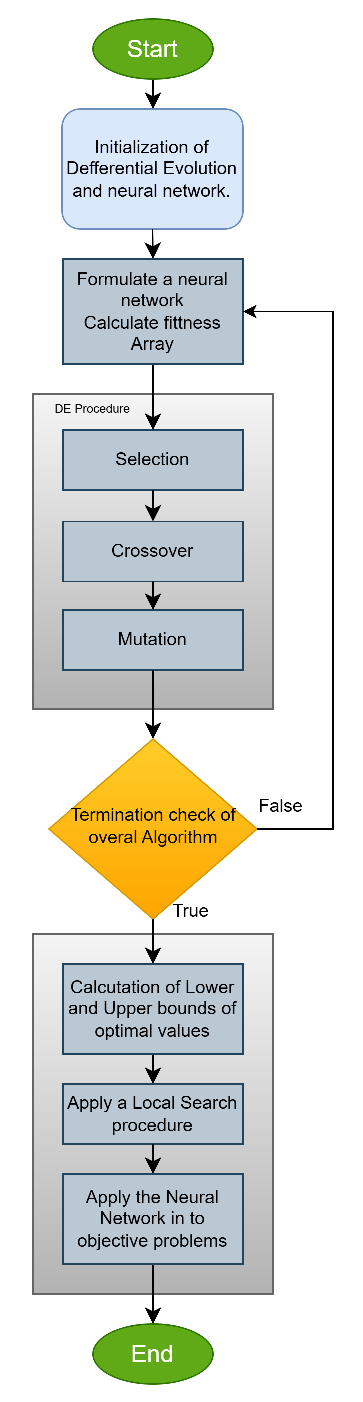
\includegraphics[scale=0.5]{neural_de.eps}
\par\end{centering}
\caption{The flowchart of the proposed method.\label{fig:flow_de}}

\end{figure}


\section{Experiments \label{sec:Experiments}}

A series of experiments were carried out to determine the effectiveness
of the proposed technique and its ability to achieve low generalization
errors in classification and data fitting problems. In addition, a
series of experiments were performed to determine the stability of
the method when critical parameters take different values. In order
to perform the experiments a series of classification and regression
datasets from the relevant literature was obtained. These datasets
cover a wide range of real - world applications, such as medicine,
physics, earth quakes, economy, signal processing etc. These datasets
can be found in the following websites:
\begin{enumerate}
\item The UCI website, \url{https://archive.ics.uci.edu/}(accessed on 9
January 2025)\citep{uci}
\item The Keel website, \url{https://sci2s.ugr.es/keel/datasets.php}(accessed
on 9 January 2025)\citep{Keel}.
\item The Statlib URL \url{https://lib.stat.cmu.edu/datasets/index}(accessed
on 9 January 2025). 
\end{enumerate}

\subsection{Experimental datasets }

The following series of classification datasets was used:
\begin{enumerate}
\item \textbf{Alcohol}, which is related to some experiments regarding alcohol
consumption \citep{alcohol}. 
\item \textbf{Australian}, which is related to bank transactions \citep{australian}.
\item \textbf{Bands,} regarding printing problems \citep{bands}.
\item \textbf{Balance} dataset \citep{balance}, which is related to psychological
experiments.
\item \textbf{Cleveland}, a medical dataset which was thoroughly studied
in the past in a series of research papers \citep{cleveland1,cleveland2}. 
\item \textbf{Circular} dataset, which created artificially. 
\item \textbf{Dermatology}, a medical dataset related to dermatology problems
\citep{dermatology}.
\item \textbf{Ecoli}, which is related to protein issues \citep{ecoli}.
\item \textbf{Haberman}, a medical dataset used for breast cancer detection.
\item \textbf{Hayes-roth} dataset \citep{hayes-roth}.
\item \textbf{Heart}, a dataset related to heart diseases \citep{heart}.
\item \textbf{HeartAttack}, a dataset related to heart diseases
\item \textbf{Hepatitis}, a medical dataset regarding hepatitis. 
\item \textbf{Housevotes}, that was used in the Congressional voting in
USA \citep{housevotes}.
\item \textbf{Ionosphere}, a dataset related to measurements from the ionosphere
\citep{ion1,ion2}.
\item \textbf{Liverdisorder}, which is a medical dataset studied in a series
of papers\citep{liver,liver1}.
\item \textbf{Lymography} \citep{lymography}.
\item \textbf{Magic}, this dataset contains measurements from physics simulations
\citep{magic}.
\item \textbf{Mammographic}, a medical dataset related to breast cancer
\citep{mammographic}.
\item \textbf{Page Blocks }dataset \citep{pageblocks}, related to the page
layout of documents.
\item \textbf{Parkinsons}, a medical dataset for the detection of Parkinson's
disease \citep{parkinsons1,parkinsons2}.
\item \textbf{Pima}, a medical dataset related to the presence of diabetes\citep{pima}.
\item \textbf{Phoneme}, a dataset regarding sounds.
\item \textbf{Popfailures}, a dataset related to measurements from climate
experiments \citep{popfailures}.
\item \textbf{Regions2}, a medical dataset used for the detection of issues
in the liver \citep{regions2}.
\item \textbf{Ring}, a dataset related to a series of multivariate normal
distributions. 
\item \textbf{Saheart}, used for the detection of heart diseases.\citep{saheart}.
\item \textbf{Segment} dataset \citep{segment}.
\item \textbf{Statheart}, a medical dataset used for the detection of heart
diseases.
\item \textbf{Sonar} dataset \citep{sonar}.
\item \textbf{Spambase}, a dataset used to recognize spam emails. 
\item \textbf{Spiral}, which is an artificial dataset.
\item \textbf{Student}, a dataset concerning experiments in schools \citep{student}.
\item \textbf{Tae}, used to evaluate teaching performance.
\item \textbf{Transfusion}, which is a medical dataset \citep{transfusion}.
\item \textbf{Wdbc}, a medical dataset which is used to detect breast cancer
\citep{wdbc1,wdbc2}.
\item \textbf{Wine}, a dataset used to detect the quality of wines \citep{wine1,wine2}.
\item \textbf{EEG} dataset, which is a medical dataset about EEG recordings\citep{eeg1,eeg2}.
The following cases from this dataset were adopted here: Z\_F\_S,
ZO\_NF\_S and ZONF\_S.
\item \textbf{Zoo}, a dataset used for animal classification \citep{zoo}
.
\end{enumerate}
Additionally, the following series of regression datasets was adopted:
\begin{enumerate}
\item \textbf{Abalone}, a dataset related to the age of abalones \citep{abalone}.
\item \textbf{Airfoil}, a dataset provided by NASA \citep{airfoil}.
\item \textbf{Auto}, a dataset related to the fuel consumption of cars.
\item \textbf{BK}, a dataset which is related to basketball games. 
\item \textbf{BL}, a dataset related to electricity experiments.
\item \textbf{Baseball}, a dataset used to estimate the income of baseball
players.
\item \textbf{Concrete}, a civil engineering dataset \citep{concrete}.
\item \textbf{DEE}, used for the prediction of electricity prices.
\item \textbf{FA}, that contains measurements about body fat.
\item \textbf{Friedman}, an artificial dataset\citep{friedman}.
\item \textbf{FY, }this dataset used in experiments regarding the longevity
of fruit flies. 
\item \textbf{HO}, a dataset with 13 features obtained from the STATLIB
repository.
\item \textbf{Housing}, used to estimate the price of houses \citep{housing}.
\item \textbf{Laser}, used in a series of laser experiments.
\item \textbf{LW}, a dataset used to detect the weight of babes.
\item \textbf{Mortgage}, an dataset related to economic measurements.
\item \textbf{Plastic}, a dataset related to problems regarding pressure
on plastics.
\item \textbf{PY }dataset, (Pyrimidines problem). The task of this dataset
is the learning of Learning Quantitative Structure Activity Relationships
(QSARs)\citep{pydataset}.
\item \textbf{Quake}, a dataset used to measure earthquakes.
\item \textbf{SN}, a dataset related to trellising and pruning.
\item \textbf{Stock}, a dataset related to the prices of stocks.
\item \textbf{Treasury}, which is related to economics.
\end{enumerate}

\subsection{Experimental results}

The code used in the current work was implemented using the C++ programming
language and the Optimus optimization library, freely available from\textbf{
}\url{https://github.com/itsoulos/OPTIMUS} (accessed on 9 January
2025). Every experiment was repeated 30 times, using different seed
for the random number generator each time. For the validation of the
experiments the 10 - fold cross validation technique was incorporated.
The machine used in the experiments was an AMD Ryzen 5950X with 128GB
of ram, running Debian Linux as the operating system. The values for
the parameters of the proposed method are listed in Table\textbf{
}\ref{tab:settings}.\textbf{ }
\begin{table}[H]
\caption{The values for the parameters of the proposed method.\label{tab:settings}}

\centering{}%
\begin{tabular}{|c|c|c|}
\hline 
PARAMETER & MEANING & VALUE\tabularnewline
\hline 
\hline 
$N_{g}$ & Number of maximum allowed generations. & 200\tabularnewline
\hline 
NP & Number of agents & 500\tabularnewline
\hline 
CR & Crossover probability & 0.9\tabularnewline
\hline 
$N_{I}$ & Number of iterations for termination rule & 10\tabularnewline
\hline 
$p_{l}$ & Local search rate & 0.005\tabularnewline
\hline 
$a$ & Weight parameter & 2.0\tabularnewline
\hline 
$H$ & Number of processing nodes for neural network & 10\tabularnewline
\hline 
\end{tabular}
\end{table}
\textbf{ }The specific values for the parameters were chosen so that
there is a compromise between the speed of the proposed method and
its efficiency. However, a series of experiments are presented below
in which various experimental parameters were modified, in order to
determine the stability of the proposed technique to possible changes
in these parameters. 

The table \ref{tab:experClass} depicts the experimental results for
the classification datasets and Table \ref{tab:experRegression} shows
the experimental results for the regression datasets.\textbf{ }The
used formula for the classification error is:
\begin{equation}
E_{C}\left(M(x)\right)=100\times\frac{\sum_{i=1}^{N}\left(\mbox{class}\left(M\left(x_{i}\right)\right)-y_{i}\right)}{N}
\end{equation}
where $M(x)$ denotes the used model and the set $T$ represents the
train dataset.\textbf{ }Likewise, the regression error is defined
as:
\begin{equation}
E_{R}\left(M(x)\right)=\frac{\sum_{i=1}^{N}\left(M\left(x_{i}\right)-y_{i}\right)^{2}}{N}
\end{equation}
In all experimental tables the following notation was adopted:
\begin{enumerate}
\item The column DATASET denotes the name of the used dataset.
\item The column ADAM represents the incorporation of the ADAM optimizer
for the training of a neural network with $H=10$ processing nodes.
\item The column BFGS stands for the usage of the BFGS optimization method
provided by Powell \citep{powell} for the training of a neural network
with~$H=10$ processing nodes.
\item The column GENETIC represents the usage of a genetic algorithm for
the training of a neural network with $H=10$ processing nodes. The
number of chromosomes in this genetic algorithm are equal with the
number of agents in the proposed method.
\item The column NEAT stands for the usage of the NEAT method (NeuroEvolution
of Augmenting Topologies ) \citep{neat} for the training of a neural
network. This method was implemented in \url{https://github.com/BiagioFesta/EvolutionNet}(accessed
on 9 January 2025). 
\item The column RBF represents the usage of a Radial Basis Function (RBF)
network \citep{rbf1,rbf2} with $H=10$ processing nodes.
\item The column PRUNE stands for the the application of OBS pruning method
\citep{prune}, as implemented in the library Fast Compressed Neural
Networks \citep{fcn}.
\item The row AVERAGE stands for the average classification or regression
error for all datasets in the corresponding table.
\end{enumerate}
The used machine learning methods cover a wide range of methods and
they have been with success in many practical problems of the related
literature.
\begin{table}[H]
\caption{Experimental results for the classification datasets using the series
of optimization methods. The numbers presented in the cells represent
the average classification error as measured for the corresponding
test set using the ten - fold cross validation method.\label{tab:experClass}}

\centering{}{\footnotesize{}}%
\begin{tabular}{|c|c|c|c|c|c|c|c|}
\hline 
{\footnotesize{}DATASET} & {\footnotesize{}ADAM} & {\footnotesize{}BFGS} & {\footnotesize{}GENETIC} & {\footnotesize{}NEAT} & {\footnotesize{}RBF} & {\footnotesize{}PRUNE} & {\footnotesize{}NEURALDE}\tabularnewline
\hline 
\hline 
{\footnotesize{}ALCOHOL} & {\footnotesize{}57.78\%} & {\footnotesize{}41.50\%} & {\footnotesize{}39.57\%} & {\footnotesize{}66.80\%} & {\footnotesize{}49.32\%} & {\footnotesize{}15.75\%} & {\footnotesize{}19.15\%}\tabularnewline
\hline 
{\footnotesize{}AUSTRALIAN} & {\footnotesize{}35.65\%} & {\footnotesize{}38.13\%} & {\footnotesize{}32.21\%} & {\footnotesize{}31.98\%} & {\footnotesize{}34.89\%} & {\footnotesize{}43.66\%} & {\footnotesize{}15.31\%}\tabularnewline
\hline 
{\footnotesize{}BALANCE} & {\footnotesize{}12.27\%} & {\footnotesize{}8.64\%} & {\footnotesize{}8.97\%} & {\footnotesize{}23.14\%} & {\footnotesize{}33.53\%} & {\footnotesize{}9.00\%} & {\footnotesize{}6.92\%}\tabularnewline
\hline 
{\footnotesize{}BANDS} & {\footnotesize{}36.92\%} & {\footnotesize{}36.67\%} & {\footnotesize{}34.92\%} & {\footnotesize{}34.30\%} & {\footnotesize{}37.17\%} & {\footnotesize{}37.68\%} & {\footnotesize{}35.00\%}\tabularnewline
\hline 
{\footnotesize{}CLEVELAND} & {\footnotesize{}67.55\%} & {\footnotesize{}77.55\%} & {\footnotesize{}51.60\%} & {\footnotesize{}53.44\%} & {\footnotesize{}67.10\%} & {\footnotesize{}51.48\%} & {\footnotesize{}45.07\%}\tabularnewline
\hline 
{\footnotesize{}CIRCULAR} & {\footnotesize{}19.95\%} & {\footnotesize{}6.08\%} & {\footnotesize{}5.99\%} & {\footnotesize{}35.18\%} & {\footnotesize{}5.98\%} & {\footnotesize{}12.76\%} & {\footnotesize{}4.23\%}\tabularnewline
\hline 
{\footnotesize{}DERMATOLOGY} & {\footnotesize{}26.14\%} & {\footnotesize{}52.92\%} & {\footnotesize{}30.58\%} & {\footnotesize{}32.43\%} & {\footnotesize{}62.34\%} & {\footnotesize{}9.02\%} & {\footnotesize{}10.38\%}\tabularnewline
\hline 
{\footnotesize{}ECOLI} & {\footnotesize{}64.43\%} & {\footnotesize{}69.52\%} & {\footnotesize{}54.67\%} & {\footnotesize{}43.44\%} & {\footnotesize{}59.48\%} & {\footnotesize{}60.32\%} & {\footnotesize{}45.22\%}\tabularnewline
\hline 
{\footnotesize{}HABERMAN} & {\footnotesize{}29.00\%} & {\footnotesize{}29.34\%} & {\footnotesize{}28.66\%} & {\footnotesize{}24.04\%} & {\footnotesize{}25.10\%} & {\footnotesize{}29.38\%} & {\footnotesize{}27.55\%}\tabularnewline
\hline 
{\footnotesize{}HAYES-ROTH} & {\footnotesize{}59.70\%} & {\footnotesize{}37.33\%} & {\footnotesize{}56.18\%} & {\footnotesize{}50.15\%} & {\footnotesize{}64.36\%} & {\footnotesize{}45.44\%} & {\footnotesize{}35.59\%}\tabularnewline
\hline 
{\footnotesize{}HEART} & {\footnotesize{}38.53\%} & {\footnotesize{}39.44\%} & {\footnotesize{}28.34\%} & {\footnotesize{}39.27\%} & {\footnotesize{}31.20\%} & {\footnotesize{}27.21\%} & {\footnotesize{}17.60\%}\tabularnewline
\hline 
{\footnotesize{}HEARTATTACK} & {\footnotesize{}45.55\%} & {\footnotesize{}46.67\%} & {\footnotesize{}29.03\%} & {\footnotesize{}32.34\%} & {\footnotesize{}29.00\%} & {\footnotesize{}29.26\%} & {\footnotesize{}19.70\%}\tabularnewline
\hline 
{\footnotesize{}HEPATITIS} & {\footnotesize{}68.13\%} & {\footnotesize{}72.47\%} & {\footnotesize{}62.12\%} & {\footnotesize{}67.04\%} & {\footnotesize{}64.63\%} & {\footnotesize{}63.40\%} & {\footnotesize{}57.46\%}\tabularnewline
\hline 
{\footnotesize{}HOUSEVOTES} & {\footnotesize{}7.48\%} & {\footnotesize{}7.13\%} & {\footnotesize{}6.62\%} & {\footnotesize{}10.89\%} & {\footnotesize{}6.13\%} & {\footnotesize{}5.81\%} & {\footnotesize{}7.48\%}\tabularnewline
\hline 
{\footnotesize{}IONOSPHERE} & {\footnotesize{}16.64\%} & {\footnotesize{}15.29\%} & {\footnotesize{}15.14\%} & {\footnotesize{}19.67\%} & {\footnotesize{}16.22\%} & {\footnotesize{}11.32\%} & {\footnotesize{}16.17\%}\tabularnewline
\hline 
{\footnotesize{}LIVERDISORDER} & {\footnotesize{}41.53\%} & {\footnotesize{}42.59\%} & {\footnotesize{}31.11\%} & {\footnotesize{}30.67\%} & {\footnotesize{}30.84\%} & {\footnotesize{}49.72\%} & {\footnotesize{}31.72\%}\tabularnewline
\hline 
{\footnotesize{}LYMOGRAPHY} & {\footnotesize{}39.79\%} & {\footnotesize{}35.43\%} & {\footnotesize{}28.42\%} & {\footnotesize{}33.70\%} & {\footnotesize{}25.50\%} & {\footnotesize{}22.02\%} & {\footnotesize{}28.86\%}\tabularnewline
\hline 
{\footnotesize{}MAGIC} & {\footnotesize{}40.55\%} & {\footnotesize{}17.30\%} & {\footnotesize{}21.75\%} & {\footnotesize{}24.85\%} & {\footnotesize{}21.28\%} & {\footnotesize{}30.76\%} & {\footnotesize{}11.73\%}\tabularnewline
\hline 
{\footnotesize{}MAMMOGRAPHIC} & {\footnotesize{}46.25\%} & {\footnotesize{}17.24\%} & {\footnotesize{}19.88\%} & {\footnotesize{}22.85\%} & {\footnotesize{}21.38\%} & {\footnotesize{}38.10\%} & {\footnotesize{}17.52\%}\tabularnewline
\hline 
{\footnotesize{}PARKINSONS} & {\footnotesize{}24.06\%} & {\footnotesize{}27.58\%} & {\footnotesize{}18.05\%} & {\footnotesize{}18.56\%} & {\footnotesize{}17.41\%} & {\footnotesize{}22.12\%} & {\footnotesize{}14.32\%}\tabularnewline
\hline 
{\footnotesize{}PAGE BLOCKS} & {\footnotesize{}34.27\%} & {\footnotesize{}8.49\%} & {\footnotesize{}6.84\%} & {\footnotesize{}10.22\%} & {\footnotesize{}10.09\%} & {\footnotesize{}12.47\%} & {\footnotesize{}6.04\%}\tabularnewline
\hline 
{\footnotesize{}PHONEME} & {\footnotesize{}29.43\%} & {\footnotesize{}15.58\%} & {\footnotesize{}15.55\%} & {\footnotesize{}22.34\%} & {\footnotesize{}23.32\%} & {\footnotesize{}29.35\%} & {\footnotesize{}15.50\%}\tabularnewline
\hline 
{\footnotesize{}PIMA} & {\footnotesize{}34.85\%} & {\footnotesize{}35.59\%} & {\footnotesize{}32.19\%} & {\footnotesize{}34.51\%} & {\footnotesize{}25.78\%} & {\footnotesize{}35.08\%} & {\footnotesize{}24.85\%}\tabularnewline
\hline 
{\footnotesize{}POPFAILURES} & {\footnotesize{}5.18\%} & {\footnotesize{}5.24\%} & {\footnotesize{}5.94\%} & {\footnotesize{}7.05\%} & {\footnotesize{}7.04\%} & {\footnotesize{}4.79\%} & {\footnotesize{}6.09\%}\tabularnewline
\hline 
{\footnotesize{}REGIONS2} & {\footnotesize{}29.85\%} & {\footnotesize{}36.28\%} & {\footnotesize{}29.39\%} & {\footnotesize{}33.23\%} & {\footnotesize{}38.29\%} & {\footnotesize{}34.26\%} & {\footnotesize{}28.77\%}\tabularnewline
\hline 
{\footnotesize{}RING} & {\footnotesize{}28.80\%} & {\footnotesize{}29.44\%} & {\footnotesize{}28.80\%} & {\footnotesize{}30.85\%} & {\footnotesize{}21.67\%} & {\footnotesize{}51.65\%} & {\footnotesize{}22.90\%}\tabularnewline
\hline 
{\footnotesize{}SAHEART} & {\footnotesize{}34.04\%} & {\footnotesize{}37.48\%} & {\footnotesize{}34.86\%} & {\footnotesize{}34.51\%} & {\footnotesize{}32.19\%} & {\footnotesize{}37.70\%} & {\footnotesize{}29.63\%}\tabularnewline
\hline 
{\footnotesize{}SEGMENT} & {\footnotesize{}49.75\%} & {\footnotesize{}68.97\%} & {\footnotesize{}57.72\%} & {\footnotesize{}66.72\%} & {\footnotesize{}59.68\%} & {\footnotesize{}60.40\%} & {\footnotesize{}15.60\%}\tabularnewline
\hline 
{\footnotesize{}SONAR} & {\footnotesize{}30.33\%} & {\footnotesize{}25.85\%} & {\footnotesize{}22.40\%} & {\footnotesize{}34.10\%} & {\footnotesize{}27.90\%} & {\footnotesize{}23.80\%} & {\footnotesize{}19.80\%}\tabularnewline
\hline 
{\footnotesize{}SPAMBASE} & {\footnotesize{}48.05\%} & {\footnotesize{}18.16\%} & {\footnotesize{}6.37\%} & {\footnotesize{}35.77\%} & {\footnotesize{}29.35\%} & {\footnotesize{}3.91\%} & {\footnotesize{}4.95\%}\tabularnewline
\hline 
{\footnotesize{}SPIRAL} & {\footnotesize{}47.67\%} & {\footnotesize{}47.99\%} & {\footnotesize{}48.66\%} & {\footnotesize{}48.66\%} & {\footnotesize{}44.87\%} & {\footnotesize{}50.38\%} & {\footnotesize{}42.06\%}\tabularnewline
\hline 
{\footnotesize{}STATHEART} & {\footnotesize{}44.04\%} & {\footnotesize{}39.65\%} & {\footnotesize{}27.25\%} & {\footnotesize{}44.36\%} & {\footnotesize{}31.36\%} & {\footnotesize{}28.37\%} & {\footnotesize{}18.53\%}\tabularnewline
\hline 
{\footnotesize{}STUDENT} & {\footnotesize{}5.13\%} & {\footnotesize{}7.14\%} & {\footnotesize{}5.61\%} & {\footnotesize{}10.20\%} & {\footnotesize{}5.49\%} & {\footnotesize{}10.84\%} & {\footnotesize{}4.86\%}\tabularnewline
\hline 
{\footnotesize{}TAE} & {\footnotesize{}60.20\%} & {\footnotesize{}51.58\%} & {\footnotesize{}49.84\%} & {\footnotesize{}60.67\%} & {\footnotesize{}60.02\%} & {\footnotesize{}60.16\%} & {\footnotesize{}45.62\%}\tabularnewline
\hline 
{\footnotesize{}TRANSFUSION} & {\footnotesize{}25.68\%} & {\footnotesize{}25.84\%} & {\footnotesize{}24.87\%} & {\footnotesize{}24.87\%} & {\footnotesize{}26.41\%} & {\footnotesize{}29.35\%} & {\footnotesize{}23.59\%}\tabularnewline
\hline 
{\footnotesize{}WDBC} & {\footnotesize{}35.35\%} & {\footnotesize{}29.91\%} & {\footnotesize{}8.56\%} & {\footnotesize{}12.88\%} & {\footnotesize{}7.27\%} & {\footnotesize{}15.48\%} & {\footnotesize{}4.29\%}\tabularnewline
\hline 
{\footnotesize{}WINE} & {\footnotesize{}29.40\%} & {\footnotesize{}59.71\%} & {\footnotesize{}19.20\%} & {\footnotesize{}25.43\%} & {\footnotesize{}31.41\%} & {\footnotesize{}16.62\%} & {\footnotesize{}10.39\%}\tabularnewline
\hline 
{\footnotesize{}Z\_F\_S} & {\footnotesize{}47.81\%} & {\footnotesize{}39.37\%} & {\footnotesize{}10.73\%} & {\footnotesize{}38.41\%} & {\footnotesize{}13.16\%} & {\footnotesize{}17.91\%} & {\footnotesize{}6.81\%}\tabularnewline
\hline 
{\footnotesize{}ZO\_NF\_S} & {\footnotesize{}47.43\%} & {\footnotesize{}43.04\%} & {\footnotesize{}21.54\%} & {\footnotesize{}43.75\%} & {\footnotesize{}9.02\%} & {\footnotesize{}15.57\%} & {\footnotesize{}4.73\%}\tabularnewline
\hline 
{\footnotesize{}ZONF\_S} & {\footnotesize{}11.99\%} & {\footnotesize{}15.62\%} & {\footnotesize{}4.36\%} & {\footnotesize{}5.44\%} & {\footnotesize{}4.03\%} & {\footnotesize{}3.27\%} & {\footnotesize{}2.41\%}\tabularnewline
\hline 
{\footnotesize{}ZOO} & {\footnotesize{}14.13\%} & {\footnotesize{}10.70\%} & {\footnotesize{}9.50\%} & {\footnotesize{}20.27\%} & {\footnotesize{}21.93\%} & {\footnotesize{}8.53\%} & {\footnotesize{}6.63\%}\tabularnewline
\hline 
\textbf{\footnotesize{}AVERAGE} & \textbf{\footnotesize{}35.88\%} & \textbf{\footnotesize{}33.43\%} & \textbf{\footnotesize{}26.19\%} & \textbf{\footnotesize{}32.66\%} & \textbf{\footnotesize{}30.08\%} & \textbf{\footnotesize{}28.39\%} & \textbf{\footnotesize{}19.78\%}\tabularnewline
\hline 
\end{tabular}{\footnotesize\par}
\end{table}
\begin{table}[H]
\caption{Experimental results for the provided regression datasets using the
series of methods. In each cell the average regression error for each
dataset is depicted. This value was calculated using ten - fold cross
validation.\label{tab:experRegression}}

\centering{}%
\begin{tabular}{|c|c|c|c|c|c|c|c|}
\hline 
{\footnotesize{}DATASET} & {\footnotesize{}ADAM} & {\footnotesize{}BFGS} & {\footnotesize{}GENETIC} & {\footnotesize{}NEAT} & {\footnotesize{}RBF} & {\footnotesize{}PRUNE} & {\footnotesize{}NEURALDE}\tabularnewline
\hline 
\hline 
{\footnotesize{}ABALONE} & {\footnotesize{}4.30} & {\footnotesize{}5.69} & {\footnotesize{}7.17} & {\footnotesize{}9.88} & {\footnotesize{}7.37} & {\footnotesize{}7.88} & {\footnotesize{}5.04}\tabularnewline
\hline 
{\footnotesize{}AIRFOIL} & {\footnotesize{}0.005} & {\footnotesize{}0.003} & {\footnotesize{}0.003} & {\footnotesize{}0.067} & {\footnotesize{}0.27} & {\footnotesize{}0.002} & {\footnotesize{}0.0014}\tabularnewline
\hline 
{\footnotesize{}AUTO} & {\footnotesize{}70.84} & {\footnotesize{}60.97} & {\footnotesize{}12.18} & {\footnotesize{}56.06} & {\footnotesize{}17.87} & {\footnotesize{}75.59} & {\footnotesize{}16.21}\tabularnewline
\hline 
{\footnotesize{}BK} & {\footnotesize{}0.0252} & {\footnotesize{}0.28} & {\footnotesize{}0.027} & {\footnotesize{}0.15} & {\footnotesize{}0.02} & {\footnotesize{}0.027} & {\footnotesize{}0.019}\tabularnewline
\hline 
{\footnotesize{}BL} & {\footnotesize{}0.622} & {\footnotesize{}2.55} & {\footnotesize{}5.74} & {\footnotesize{}0.05} & {\footnotesize{}0.013} & {\footnotesize{}0.027} & {\footnotesize{}0.016}\tabularnewline
\hline 
{\footnotesize{}BASEBALL} & {\footnotesize{}77.90} & {\footnotesize{}119.63} & {\footnotesize{}103.60} & {\footnotesize{}100.39} & {\footnotesize{}93.02} & {\footnotesize{}94.50} & {\footnotesize{}60.56}\tabularnewline
\hline 
{\footnotesize{}CONCRETE} & {\footnotesize{}0.078} & {\footnotesize{}0.066} & {\footnotesize{}0.0099} & {\footnotesize{}0.081} & {\footnotesize{}0.011} & {\footnotesize{}0.0077} & {\footnotesize{}0.003}\tabularnewline
\hline 
{\footnotesize{}DEE} & {\footnotesize{}0.63} & {\footnotesize{}2.36} & {\footnotesize{}1.013} & {\footnotesize{}1.51} & {\footnotesize{}0.17} & {\footnotesize{}1.08} & {\footnotesize{}0.35}\tabularnewline
\hline 
{\footnotesize{}FA} & {\footnotesize{}0.048} & {\footnotesize{}0.426} & {\footnotesize{}0.025} & {\footnotesize{}0.19} & {\footnotesize{}0.015} & {\footnotesize{}0.029} & {\footnotesize{}0.083}\tabularnewline
\hline 
{\footnotesize{}FRIEDMAN} & {\footnotesize{}22.90} & {\footnotesize{}1.263} & {\footnotesize{}1.249} & {\footnotesize{}19.35} & {\footnotesize{}7.23} & {\footnotesize{}8.69} & {\footnotesize{}1.22}\tabularnewline
\hline 
{\footnotesize{}HO} & {\footnotesize{}0.035} & {\footnotesize{}0.62} & {\footnotesize{}2.78} & {\footnotesize{}0.17} & {\footnotesize{}0.03} & {\footnotesize{}0.03} & {\footnotesize{}0.017}\tabularnewline
\hline 
{\footnotesize{}HOUSING} & {\footnotesize{}80.99} & {\footnotesize{}97.38} & {\footnotesize{}43.26} & {\footnotesize{}56.49} & {\footnotesize{}57.68} & {\footnotesize{}52.25} & {\footnotesize{}24.82}\tabularnewline
\hline 
{\footnotesize{}LASER} & {\footnotesize{}0.03} & {\footnotesize{}0.015} & {\footnotesize{}0.59} & {\footnotesize{}0.084} & {\footnotesize{}0.03} & {\footnotesize{}0.007} & {\footnotesize{}0.0026}\tabularnewline
\hline 
{\footnotesize{}LW} & {\footnotesize{}0.028} & {\footnotesize{}2.98} & {\footnotesize{}1.90} & {\footnotesize{}0.17} & {\footnotesize{}0.03} & {\footnotesize{}0.02} & {\footnotesize{}0.021}\tabularnewline
\hline 
{\footnotesize{}MORTGAGE} & {\footnotesize{}9.24} & {\footnotesize{}8.23} & {\footnotesize{}2.41} & {\footnotesize{}14.11} & {\footnotesize{}1.45} & {\footnotesize{}12.96} & {\footnotesize{}0.54}\tabularnewline
\hline 
{\footnotesize{}PLASTIC} & {\footnotesize{}11.71} & {\footnotesize{}20.32} & {\footnotesize{}2.791} & {\footnotesize{}20.77} & {\footnotesize{}8.62} & {\footnotesize{}17.33} & {\footnotesize{}3.27}\tabularnewline
\hline 
{\footnotesize{}PY} & {\footnotesize{}0.321} & {\footnotesize{}0.578} & {\footnotesize{}0.56} & {\footnotesize{}0.075} & {\footnotesize{}0.012} & {\footnotesize{}0.023} & {\footnotesize{}0.11}\tabularnewline
\hline 
{\footnotesize{}QUAKE} & {\footnotesize{}0.07} & {\footnotesize{}0.42} & {\footnotesize{}0.04} & {\footnotesize{}0.298} & {\footnotesize{}0.07} & {\footnotesize{}0.04} & {\footnotesize{}0.042}\tabularnewline
\hline 
{\footnotesize{}SN} & {\footnotesize{}0.026} & {\footnotesize{}0.40} & {\footnotesize{}2.95} & {\footnotesize{}0.174} & {\footnotesize{}0.027} & {\footnotesize{}0.032} & {\footnotesize{}0.027}\tabularnewline
\hline 
{\footnotesize{}STOCK} & {\footnotesize{}180.89} & {\footnotesize{}302.43} & {\footnotesize{}3.88} & {\footnotesize{}215.82} & {\footnotesize{}12.23} & {\footnotesize{}39.08} & {\footnotesize{}3.40}\tabularnewline
\hline 
{\footnotesize{}TREASURY} & {\footnotesize{}11.16} & {\footnotesize{}9.91} & {\footnotesize{}2.93} & {\footnotesize{}15.52} & {\footnotesize{}2.02} & {\footnotesize{}13.76} & {\footnotesize{}1.021}\tabularnewline
\hline 
\textbf{\footnotesize{}AVERAGE} & \textbf{\footnotesize{}22.47} & \textbf{\footnotesize{}30.31} & \textbf{\footnotesize{}9.29} & \textbf{\footnotesize{}24.35} & \textbf{\footnotesize{}9.91} & \textbf{\footnotesize{}15.40} & \textbf{\footnotesize{}5.56}\tabularnewline
\hline 
\end{tabular}
\end{table}

The analysis of Table \ref{tab:experClass} evaluates the error rates
of various machine learning models across multiple classification
datasets. Each row corresponds to a dataset, and each column represents
a specific model. The values indicate the error percentages, where
lower values signify better performance. The last row provides the
average error rate for each model, offering an overall performance
summary. Starting with the averages, the NEURALDE model exhibits the
best overall performance, achieving the lowest mean error rate of
19.78\%. It is followed by GENETIC with an average error rate of 26.19\%
and RBF at 30.08\%. The PRUNE model achieves an average error rate
of 28.39\%, placing it between RBF and NEAT, which has an average
error rate of 32.66\%. Meanwhile, BFGS and ADAM display the highest
average error rates, 33.43\% and 35.88\%, respectively, making NEURALDE
the most efficient model among those compared. On a dataset-specific
level, NEURALDE consistently delivers the lowest error rates in numerous
cases. For instance, in the ALCOHOL dataset, NEURALDE achieves the
best result with an error rate of 19.15\%, while PRUNE follows closely
with 15.75\%, outperforming all other models. In the CIRCULAR dataset,
NEURALDE outperforms all other models with an error rate of 4.23\%,
while PRUNE records a slightly higher error rate of 12.76\%, still
surpassing many other methods. In datasets like MAGIC and MAMMOGRAPHIC,
NEURALDE again proves superior, with error rates of 11.73\% and 17.52\%,
respectively. PRUNE, however, shows significant variability; for example,
it records 30.76\% in MAGIC, which is higher than GENETIC (21.75\%),
but still manages competitive performance in MAMMOGRAPHIC with 38.10\%.
There are, however, a few datasets where NEURALDE does not perform
as dominantly. For example, in the HOUSEVOTES dataset, it ties with
other models at 7.48\%. PRUNE performs better here with an error rate
of 5.81\%, showcasing its strengths in specific datasets. Similarly,
in the ZONF\_S dataset, NEURALDE achieves 2.41\%, while PRUNE closely
follows with 3.27\%. Despite this, NEURALDE's superior consistency
across datasets remains evident. Other models, such as GENETIC, show
strong performance in isolated cases, such as in the SPIRAL dataset
(48.66\%). However, they generally fall short of NEURALDE’s consistent
excellence. RBF demonstrates strong stability, with notable results
in the DERMATOLOGY (62.34\%) and PHONEME (23.32\%) datasets, but PRUNE
again outshines RBF in specific cases like DERMATOLOGY with an error
rate of 9.02\%. Meanwhile, ADAM and BFGS tend to underperform, particularly
in datasets like SPAMBASE, where they record high error rates of 48.05\%
and 18.16\%, respectively. PRUNE outperforms them significantly in
SPAMBASE with an error rate of just 3.91\%, illustrating its competitiveness
in certain scenarios.In conclusion, the NEURALDE model stands out
as the most effective model overall, achieving the lowest average
error rate and excelling in the majority of datasets. PRUNE emerges
as a strong contender, with competitive performance and notable success
in certain datasets. While other models, such as RBF and GENETIC,
perform well in specific scenarios, NEURALDE demonstrates superior
consistency and effectiveness across a wide range of datasets, with
PRUNE providing significant value in enhancing classification accuracy
in many cases.

The Table \ref{tab:experRegression} presents the performance of various
machine learning models on regression problems, where the values represent
the error. Lower error values indicate better performance. Each row
corresponds to a specific dataset, while the last row shows the average
error for each model, providing an overall view of their effectiveness.
Based on the average error, NEURALDE demonstrates the best performance,
with the lowest overall error of 5.56. This result suggests that the
model consistently performs well across most datasets. PRUNE follows
as the second-best model, with an average error of 15.40, outperforming
GENETIC, RBF, and other methods in several cases. GENETIC and RBF
achieve average errors of 9.29 and 9.91, respectively. ADAM, NEAT,
and BFGS exhibit higher average errors, at 22.47, 24.35, and 30.31
respectively, indicating lower performance compared to the other models.
Analyzing the results dataset by dataset, NEURALDE records the smallest
error in several cases. For instance, in the AIRFOIL dataset, it achieves
an error of 0.0014, outperforming all other models. PRUNE also shows
strong performance here, with an error of 0.002, close to NEURALDE.
In the CONCRETE dataset, NEURALDE achieves the lowest error of 0.003,
while PRUNE achieves the second-lowest error of 0.0077, further confirming
its reliability. Similarly, in the LASER dataset, NEURALDE delivers
an exceptionally low error of 0.0026, followed closely by PRUNE with
an error of 0.007. In the TREASURY dataset, NEURALDE demonstrates
superior performance with an error of 1.021, better than all other
models, while PRUNE also achieves a competitive error of 13.76, outperforming
NEAT and ADAM. PRUNE shows notable performance in several datasets
where it surpasses other models. For instance, in the STOCK dataset,
PRUNE records an error of 39.08, which is lower than NEAT (215.82)
and ADAM (180.89), though slightly higher than NEURALDE (3.40). In
the BASEBALL dataset, PRUNE achieves 94.50, outperforming ADAM (77.90)
and NEAT (100.39). In the MORTGAGE dataset, PRUNE achieves an error
of 12.96, which, while not the lowest, still outperforms several other
models including NEAT (14.11) and ADAM (9.24). Overall, while NEURALDE
stands out as the most effective model, PRUNE emerges as a highly
competitive alternative, consistently delivering strong results across
multiple datasets. GENETIC and RBF also perform well in specific cases,
but their performance is less consistent compared to NEURALDE and
PRUNE. ADAM, NEAT, and BFGS generally underperform relative to the
other methods. 

In Figure \ref{fig:statClass}, the comparison of the proposed machine
learning model NEURALDE with other models for classification datasets
is illustrated, based on the values of the critical parameter p, which
indicate the levels of statistical significance. The results show
exceptionally low p-values, suggesting that the differences in the
performance of NEURALDE compared to other models are not random and
are statistically highly significant. Specifically, the comparison
of NEURALDE with ADAM yielded p=4.7e-08, with BFGS p=1e\textminus 10,
with GENETIC p=2.9e\textminus 09, with NEAT p=2.3e\textminus 10, with
RBF p=1.3e\textminus 08, and with PRUNE p=5.8e\textminus 08. These
values are well below the common thresholds of significance (p\textless 0.05
: significant), indicating that the superiority of NEURALDE is statistically
well-founded. The results confirm the high efficiency of the proposed
model compared to other machine learning methods, demonstrating its
reliability and effectiveness in classification problems.

\begin{figure}[H]
\begin{centering}
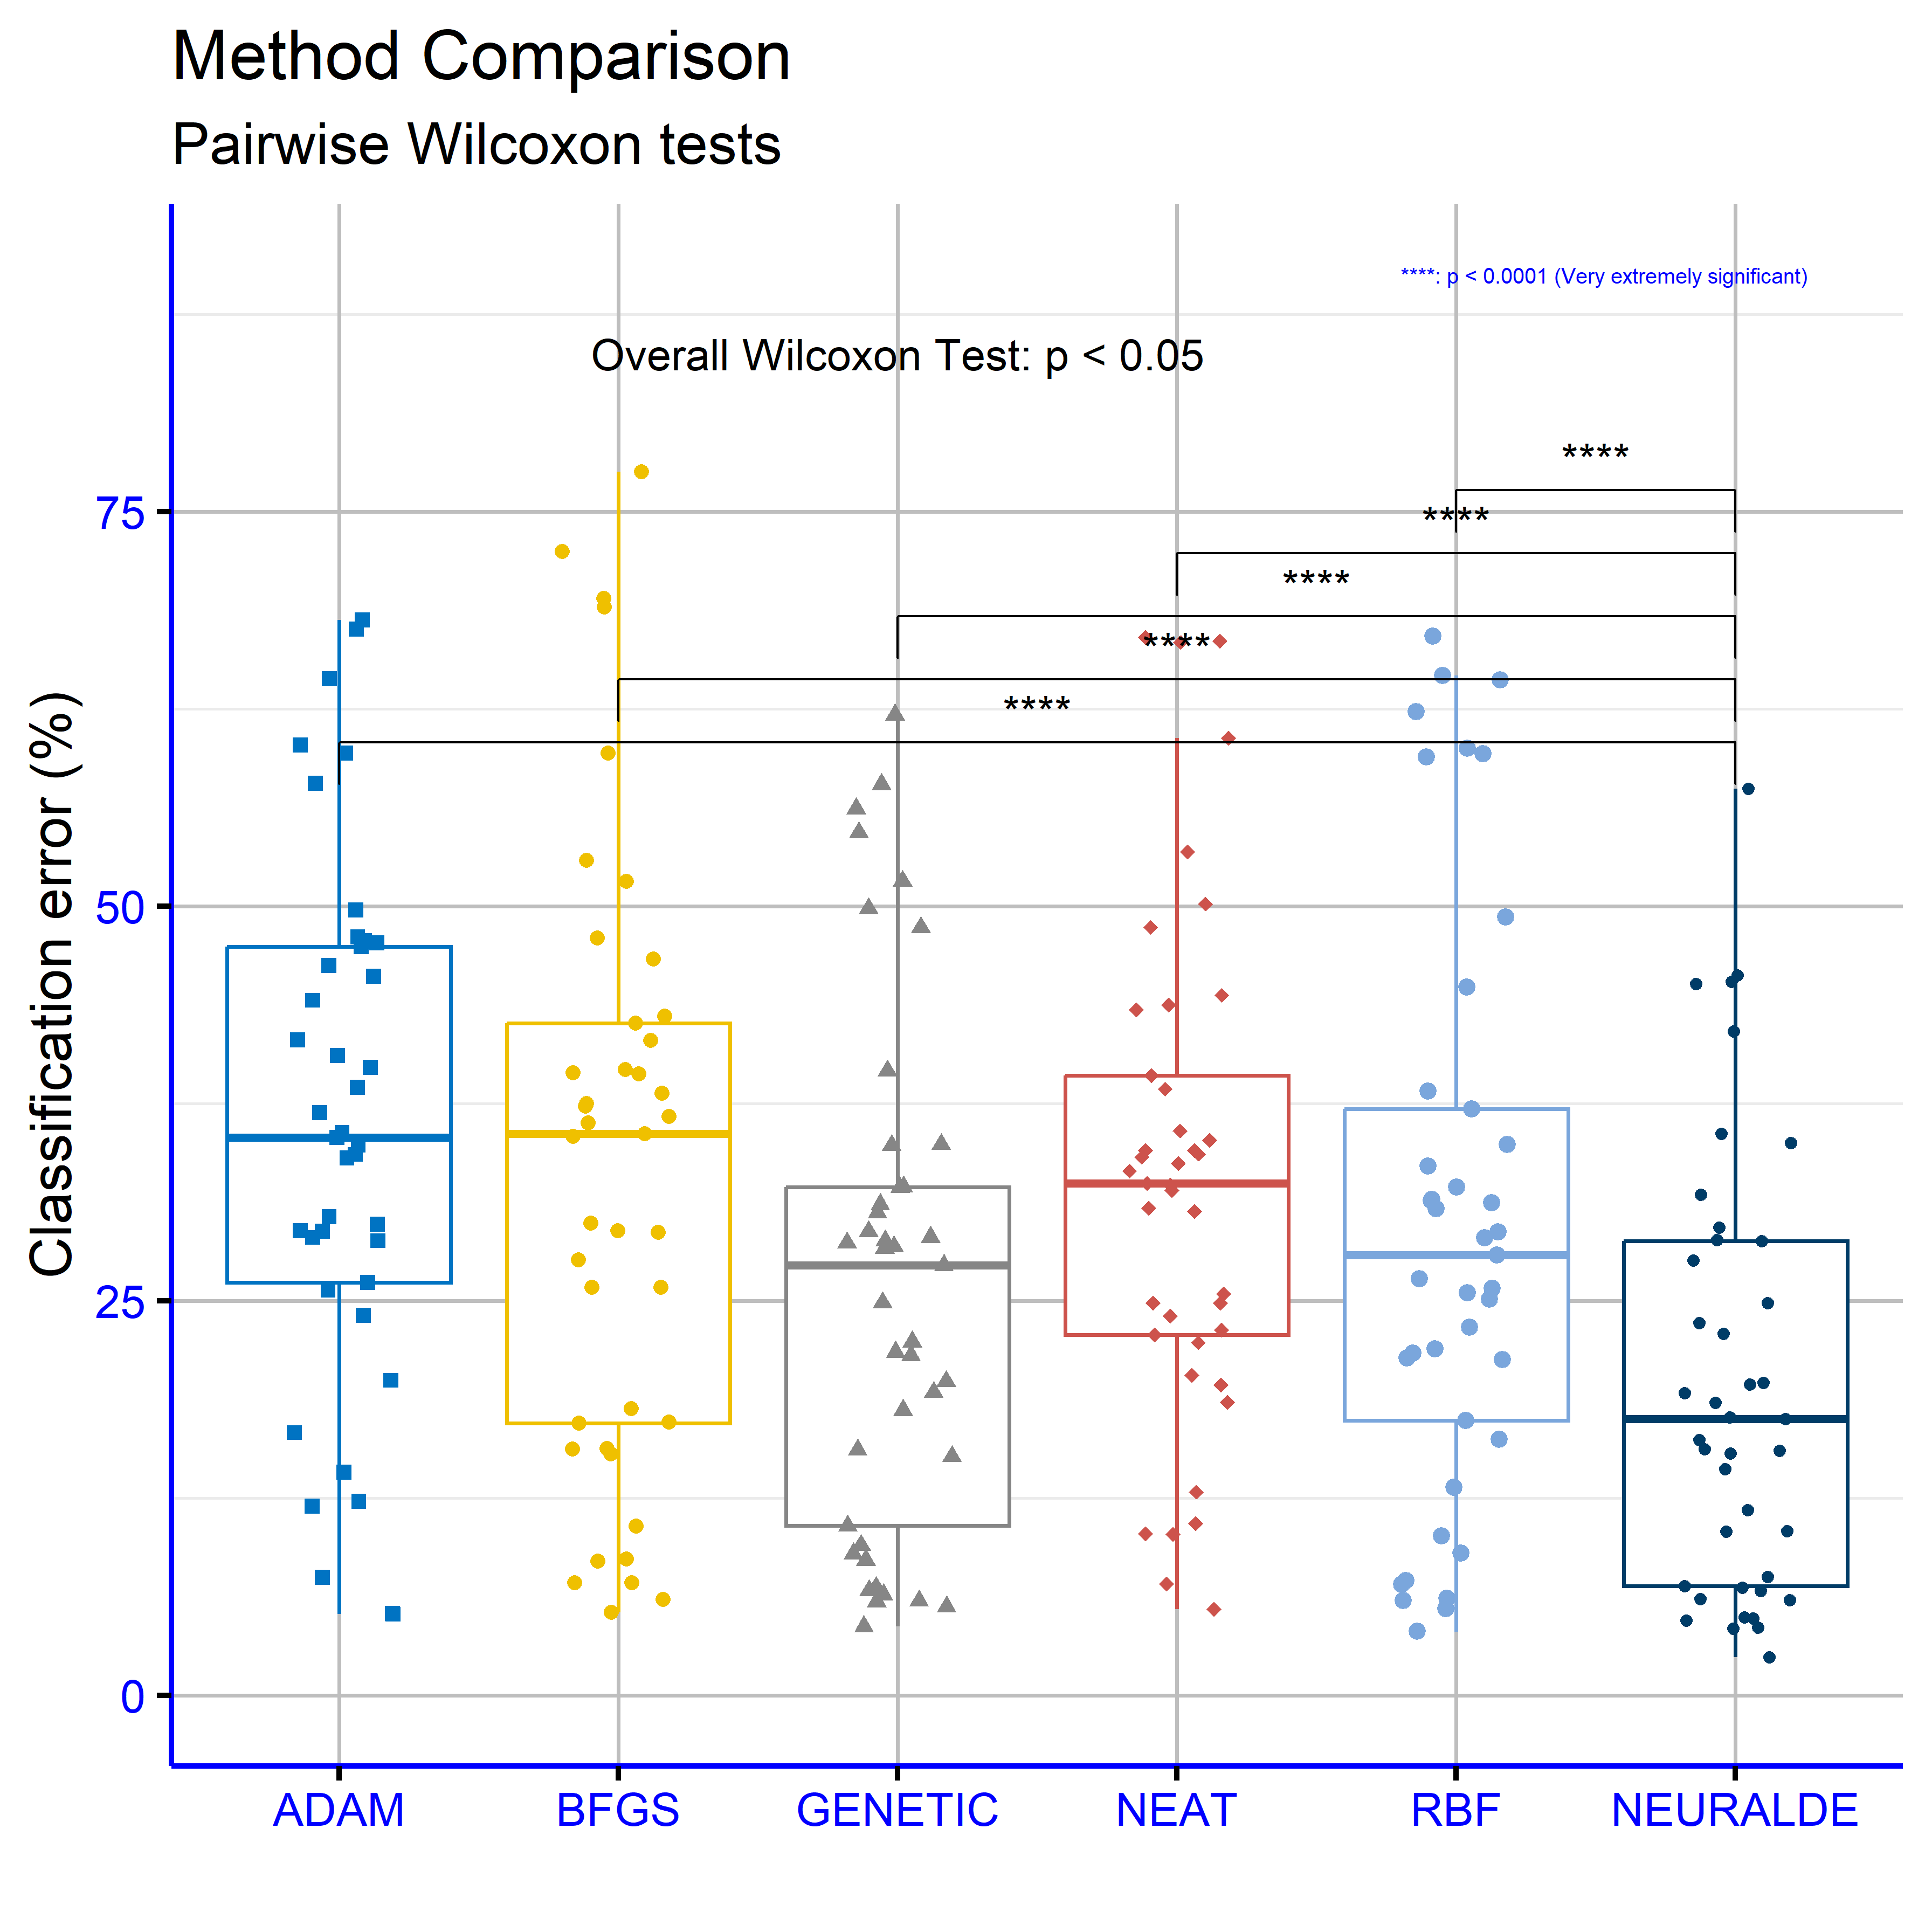
\includegraphics[scale=0.5]{s1}
\par\end{centering}
\caption{Statistical comparison of the used machine learning models for the
classification datasets.\label{fig:statClass}}

\end{figure}

Similarly, the comparison of the proposed model with others in regression
problems highlighted NEURALDE as the most efficient model. Specifically,
the comparison of NEURALDE with ADAM yielded p=0.00051, with BFGS
p=9.5e\textminus 07, with GENETIC p=0.0033, with NEAT p=2.9e\textminus 06,
with RBF p=0.0048, and with PRUNE p=0.001. These values confirm the
statistical significance of the differences, indicating that the superiority
of NEURALDE in regression problems is well-documented and not random,
as shown in Figure \ref{fig:statRegression}.

\begin{figure}[H]
\begin{centering}
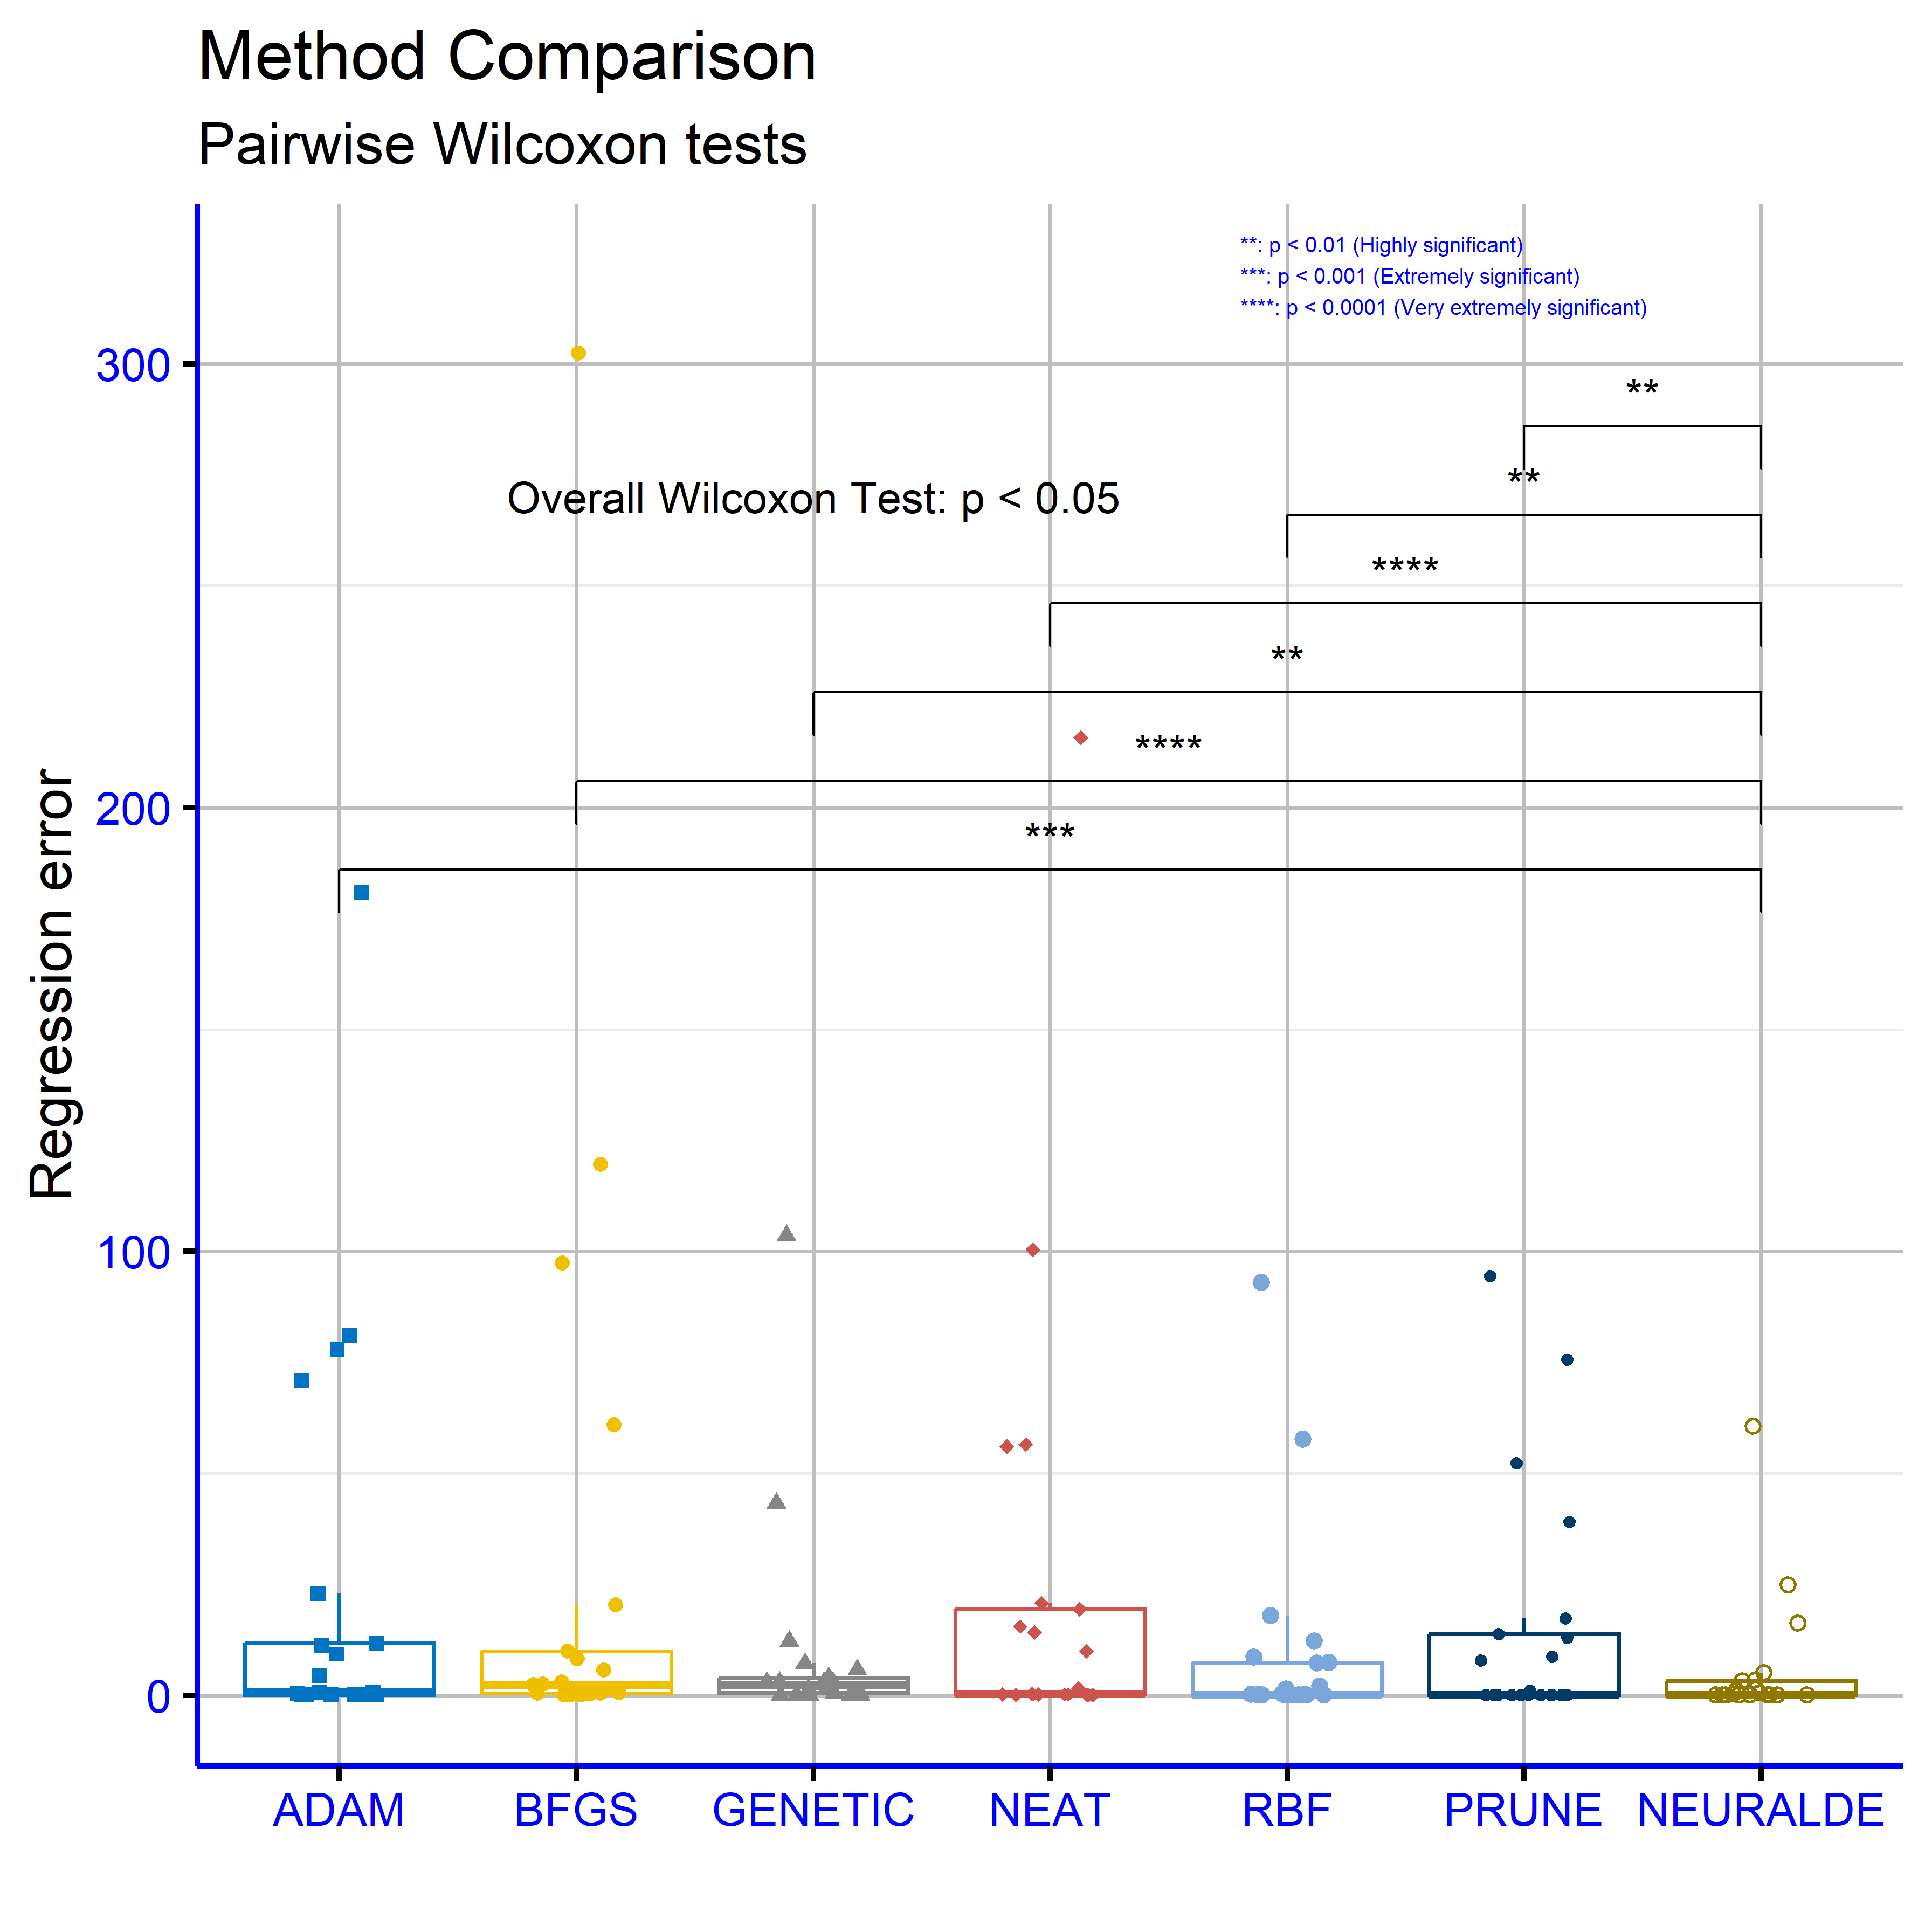
\includegraphics[scale=0.5]{s2}
\par\end{centering}
\caption{Statistical comparison between the machine learning models for the
regression datasets.\label{fig:statRegression}}

\end{figure}
 Furthermore, the average classification error for the methods used
in the experiments is presented in Figure \ref{fig:averageClass},
where the dynamics of the new technique are clearly depicted. 

\begin{figure}[H]
\begin{centering}
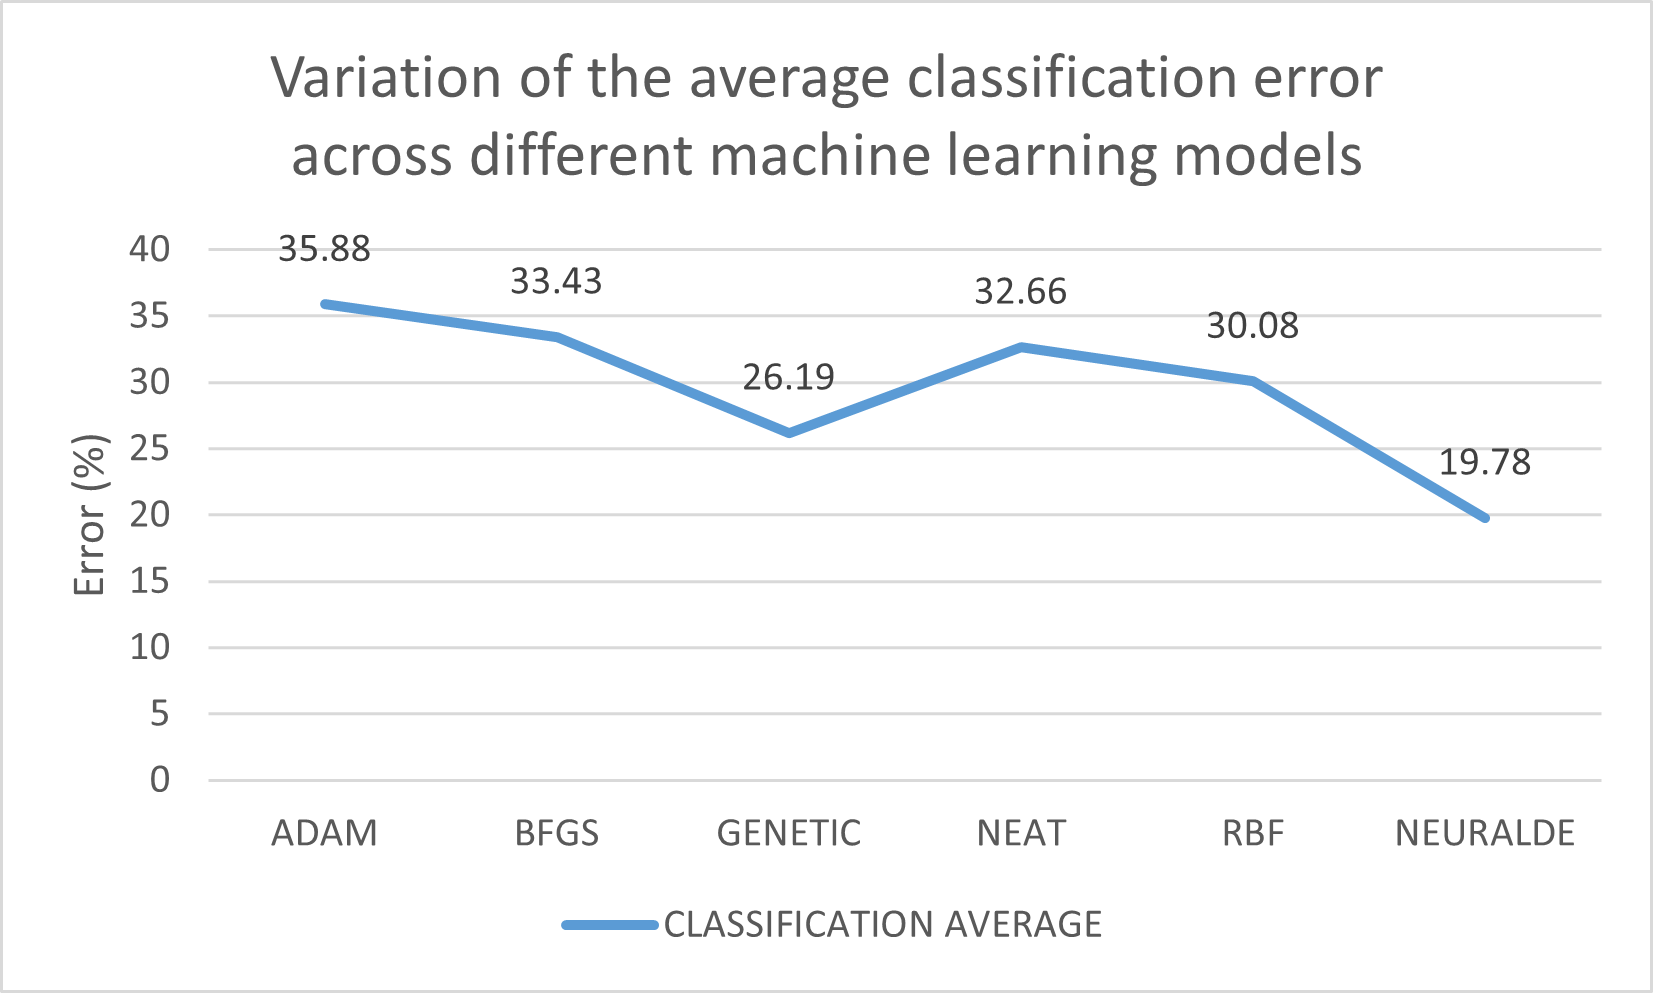
\includegraphics{classificationAVG}
\par\end{centering}
\caption{The average classification error for all methods used in the conducted
experiments.\label{fig:averageClass}}

\end{figure}
Likewise, the average regression error for all used techniques is
depicted in Figure \ref{fig:averageRegression}.

\begin{figure}[H]
\begin{centering}
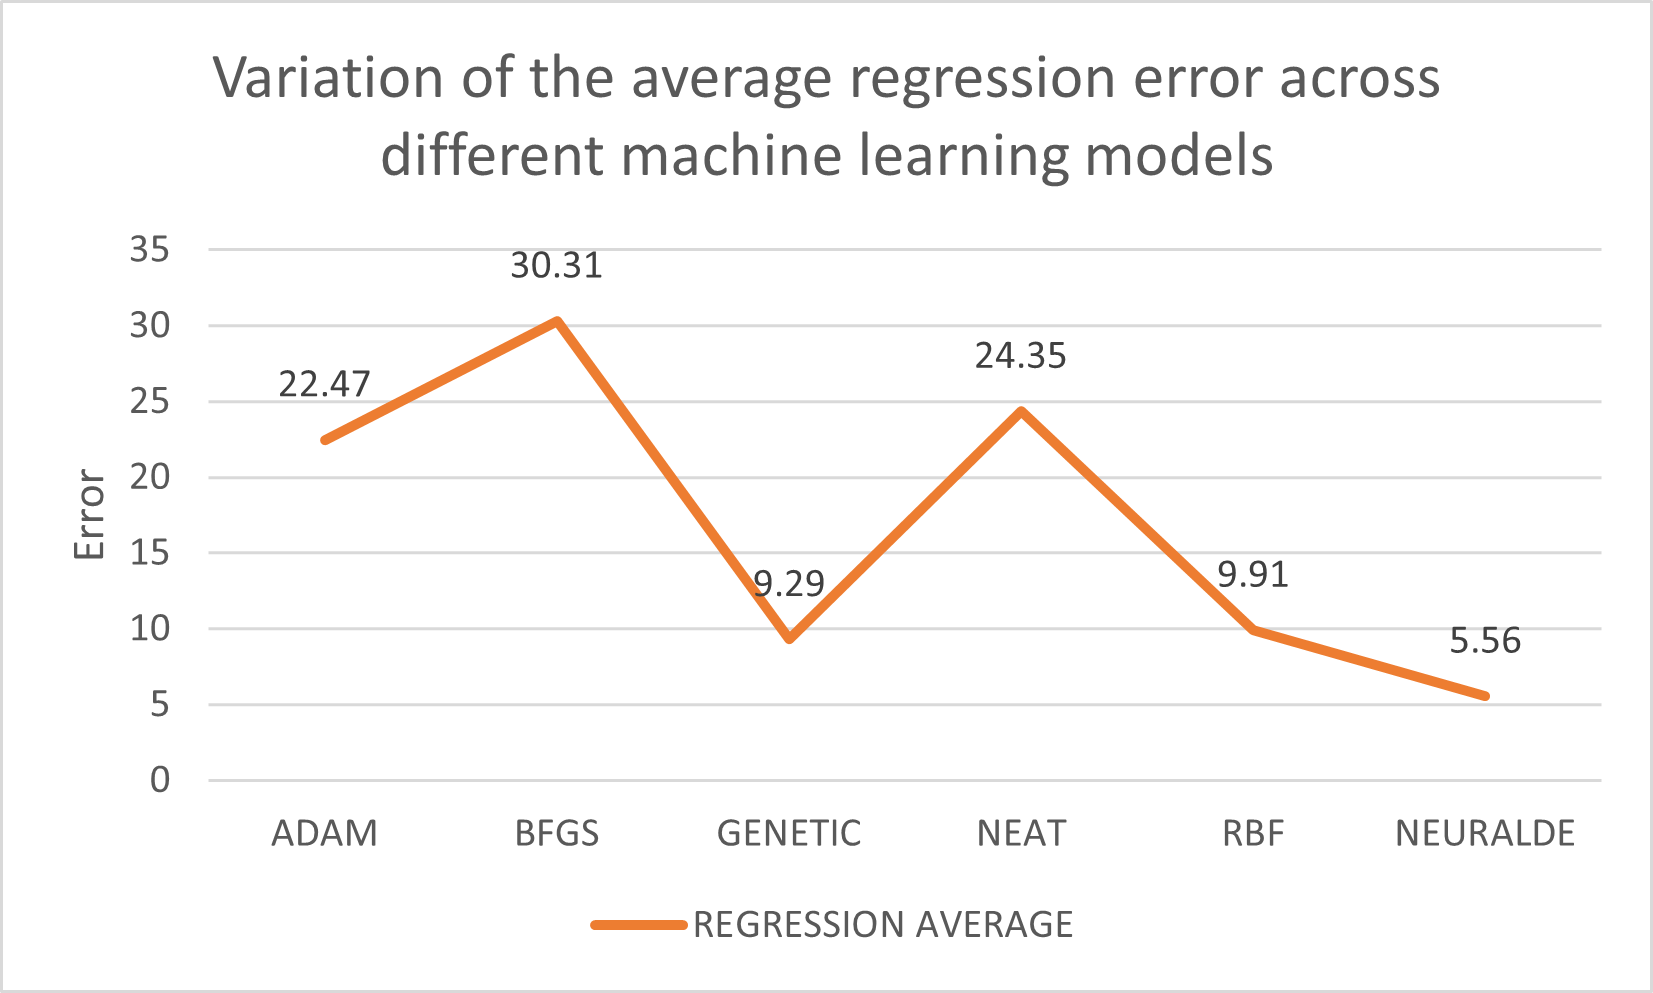
\includegraphics{regressionAVG}
\par\end{centering}
\caption{Average regression error for the used techniques.\label{fig:averageRegression}}

\end{figure}
Finally, the average execution time for all method involved in the
conducted experiments regarding the classification datsetsets is graphically
outlined in Figure \ref{fig:de_time}.
\begin{figure}[H]
\begin{centering}
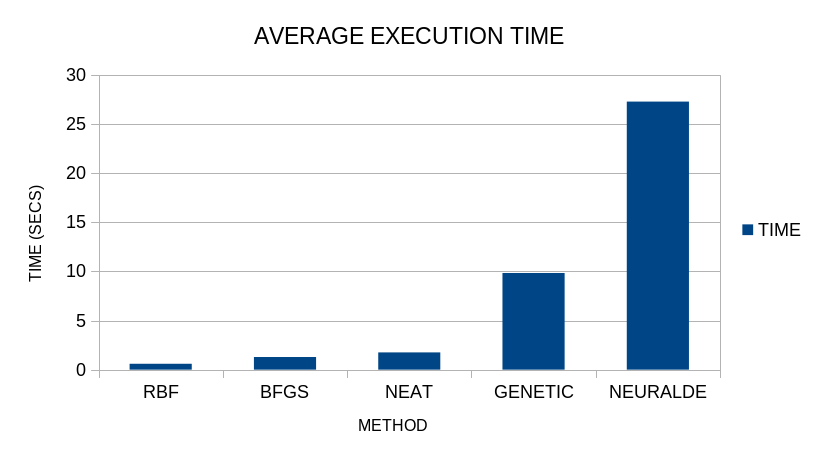
\includegraphics[scale=0.5]{neuralde_time}
\par\end{centering}
\caption{Average execution time for the machine learning methods used in the
experiments involving the classification datasets.\label{fig:de_time}}

\end{figure}
As it was expected, the proposed method requires significantly more
computation time than other method due to its complexity in the calculations
and the requirement of the periodical application of a local optimization
method.

\subsubsection{Experiments with the differential weight }

Another series of experiments was carried out in order to determine
the effect that the specific differential weight calculation mechanism
has on the accuracy of the proposed technique. For this reason the
following methods for the calculation of the differential weight (parameter
$F$) were used:
\begin{itemize}
\item The method denoted as MIGRANT in the experimental tables. In this
case the differential weight mechanism proposed in \citep{de_migrant}
was used.
\item The method denoted as ADAPTIVE in the experimental tables. This method
uses the differential weight calculation proposed in \citep{de_dynamic}.
\item The method represented as RANDOM in the experimental tables. This
method is the default method, suggested by Charilogis \citep{de_char}. 
\end{itemize}
The table \ref{tab:experFClass} provides the performance of three
differential weight computation methods (MIGRANT, ADAPTIVE, and RANDOM)
on the series of classification datasets. The analysis reveals that
the MIGRANT method achieves the smallest average error rate of 19.34\%,
indicating the best overall performance among the three methods. The
RANDOM method follows closely with an average error rate of 19.78\%,
while the ADAPTIVE method has the highest average error rate of 19.98\%,
suggesting it is the least effective on average. Examining individual
datasets, MIGRANT outperforms the other methods in several cases.
For example, in the HEART dataset, MIGRANT records an error rate of
19.01\%, better than ADAPTIVE (17.29\%) and RANDOM (17.60\%). Similarly,
in the MAGIC dataset, MIGRANT achieves a competitive error rate of
11.83\%, which is close to RANDOM (11.73\%) but higher than ADAPTIVE
(11.28\%). MIGRANT also has the lowest error in datasets such as ALCOHOL
(19.62\%), REGIONS2 (26.26\%), and SPAMBASE (5.87\%). ADAPTIVE demonstrates
strong performance in specific datasets, achieving the lowest error
rates in cases such as MAGIC (11.28\%) and HEART (17.29\%). However,
in many datasets, it performs worse than MIGRANT or RANDOM, such as
in SPAMBASE, where it records a lower error rate of 4.78\% but is
generally outperformed in other critical datasets. The RANDOM method
exhibits competitive performance in several datasets, achieving the
lowest error rates in examples like ZOO (6.63\%) and ZONF\_S (2.41\%).
However, its performance fluctuates more significantly, with higher
error rates in datasets such as HEARTATTACK (19.70\%) and REGIONS2
(28.77\%), where it is outperformed by MIGRANT and ADAPTIVE. Notable
observations include cases where the error rates are very close across
the methods, such as in datasets like CIRCULAR, where the differences
are minimal (MIGRANT at 4.28\%, ADAPTIVE at 4.34\%, and RANDOM at
4.23\%). In other cases, the differences are more pronounced, as in
SEGMENT, where MIGRANT achieves 9.71\%, significantly better than
ADAPTIVE (15.99\%) and RANDOM (15.60\%). Overall, MIGRANT demonstrates
the most consistent and robust performance across the datasets, with
the lowest average error and competitive results in many individual
datasets. RANDOM and ADAPTIVE have comparable average errors but show
more variability in their performance.

\begin{table}[H]
\caption{Experimental results for the classification datasets using a list
of proposed differential weight mechanisms found in the literature.
Each column denotes a different weight mechanism and numbers in cells
stand for the average classification error as measured on the corresponding
test set. \label{tab:experFClass}}

\centering{}%
\begin{tabular}{|c|c|c|c|}
\hline 
DATASET & MIGRANT & ADAPTIVE & RANDOM\tabularnewline
\hline 
\hline 
ALCOHOL & 19.62\% & 18.44\% & 19.15\%\tabularnewline
\hline 
AUSTRALIAN & 14.77\% & 16.14\% & 15.31\%\tabularnewline
\hline 
BALANCE & 6.79\% & 6.94\% & 6.92\%\tabularnewline
\hline 
BANDS & 33.28\% & 35.42\% & 35.00\%\tabularnewline
\hline 
CLEVELAND & 45.74\% & 44.60\% & 45.07\%\tabularnewline
\hline 
CIRCULAR & 4.28\% & 4.34\% & 4.23\%\tabularnewline
\hline 
DERMATOLOGY & 11.41\% & 9.83\% & 10.38\%\tabularnewline
\hline 
ECOLI & 42.61\% & 47.51\% & 45.22\%\tabularnewline
\hline 
HABERMAN & 27.76\% & 28.35\% & 27.55\%\tabularnewline
\hline 
HAYES-ROTH & 35.92\% & 36.31\% & 35.59\%\tabularnewline
\hline 
HEART & 19.01\% & 17.29\% & 17.60\%\tabularnewline
\hline 
HEARTATTACK & 21.31\% & 20.28\% & 19.70\%\tabularnewline
\hline 
HEPATITIS & 56.37\% & 56.46\% & 57.46\%\tabularnewline
\hline 
HOUSEVOTES & 7.47\% & 7.54\% & 7.48\%\tabularnewline
\hline 
IONOSPHERE & 15.88\% & 16.40\% & 16.17\%\tabularnewline
\hline 
LIVERDISORDER & 32.56\% & 32.54\% & 31.72\%\tabularnewline
\hline 
LYMOGRAPHY & 26.52\% & 28.95\% & 28.86\%\tabularnewline
\hline 
MAGIC & 11.83\% & 11.28\% & 11.73\%\tabularnewline
\hline 
MAMMOGRAPHIC & 17.69\% & 17.44\% & 17.52\%\tabularnewline
\hline 
PARKINSONS & 13.28\% & 14.21\% & 14.32\%\tabularnewline
\hline 
PAGE BLOCKS & 5.48\% & 5.93\% & 6.04\%\tabularnewline
\hline 
PHONEME & 15.39\% & 15.17\% & 15.50\%\tabularnewline
\hline 
PIMA & 25.04\% & 23.28\% & 24.85\%\tabularnewline
\hline 
POPFAILURES & 5.55\% & 6.55\% & 6.09\%\tabularnewline
\hline 
REGIONS2 & 26.26\% & 28.98\% & 28.77\%\tabularnewline
\hline 
RING & 21.04\% & 25.54\% & 22.90\%\tabularnewline
\hline 
SAHEART & 29.94\% & 29.80\% & 29.63\%\tabularnewline
\hline 
SEGMENT & 9.71\% & 15.99\% & 15.60\%\tabularnewline
\hline 
SONAR & 18.83\% & 18.93\% & 19.80\%\tabularnewline
\hline 
SPAMBASE & 5.87\% & 4.78\% & 4.95\%\tabularnewline
\hline 
SPIRAL & 41.36\% & 41.54\% & 42.06\%\tabularnewline
\hline 
STATHEART & 20.79\% & 19.32\% & 18.53\%\tabularnewline
\hline 
STUDENT & 4.36\% & 5.28\% & 4.86\%\tabularnewline
\hline 
TAE & 45.09\% & 44.78\% & 45.62\%\tabularnewline
\hline 
TRANSFUSION & 23.01\% & 24.51\% & 23.59\%\tabularnewline
\hline 
WDBC & 3.80\% & 4.55\% & 4.29\%\tabularnewline
\hline 
WINE & 8.22\% & 12.84\% & 10.39\%\tabularnewline
\hline 
Z\_F\_S & 7.16\% & 7.15\% & 6.81\%\tabularnewline
\hline 
ZO\_NF\_S & 4.19\% & 4.70\% & 4.73\%\tabularnewline
\hline 
ZONF\_S & 2.47\% & 2.44\% & 2.41\%\tabularnewline
\hline 
ZOO & 5.23\% & 6.87\% & 6.63\%\tabularnewline
\hline 
\textbf{AVERAGE} & \textbf{19.34\%} & \textbf{19.98\%} & \textbf{19.78\%}\tabularnewline
\hline 
\end{tabular}
\end{table}

The Table \ref{tab:experFWeightRegression} presents the performance
of three differential weight computation methods (MIGRANT, ADAPTIVE,
and RANDOM) on the regression datasets. The RANDOM method achieves
the lowest average error, 5.56, making it the most effective overall.
ADAPTIVE follows with an average error of 6.23, while MIGRANT exhibits
the highest average error at 8.03, indicating the least effective
performance. For specific datasets, RANDOM often outperforms the others.
For instance, in the HOUSING dataset, it records an error of 24.82,
lower than MIGRANT (14.58) and ADAPTIVE (32.62). Similarly, in the
PLASTIC dataset, RANDOM achieves the smallest error of 3.27 compared
to MIGRANT (5.36) and ADAPTIVE (3.57). RANDOM also shows superior
performance in datasets like MORTGAGE (0.54) and STOCK (3.4). ADAPTIVE
demonstrates strong performance in certain datasets, such as FRIEDMAN,
where its error is 1.32, outperforming MIGRANT (1.66) and RANDOM (1.22).
In the QUAKE dataset, ADAPTIVE records the lowest error of 0.041.
However, its performance is noticeably weaker in other datasets, like
HOUSING, where it registers the highest error of the three. MIGRANT
outperforms in a few cases, such as the BL dataset, where its error
is 0.007, significantly lower than ADAPTIVE (0.019) and RANDOM (0.016).
However, it generally records higher errors in many datasets, such
as AUTO (45.37) and BASEBALL (79.24), where the other methods perform
better. In some cases, such as the LASER dataset, all methods perform
similarly, with errors of 0.0026 for MIGRANT and RANDOM, and 0.0027
for ADAPTIVE. In the QUAKE dataset, the differences are also minimal,
with RANDOM having the highest error (0.042), but very close to the
others. Overall, RANDOM emerges as the most reliable and effective
method, with the lowest average error and frequent superiority across
individual datasets. ADAPTIVE performs well in selected datasets but
shows greater variability, while MIGRANT demonstrates the least effective
performance, with higher errors across numerous datasets. 

\begin{table}[H]
\caption{Experimental results for the regression datasets using a variety of
differential weigh methods. In every column a different weight mechanism
is depicted and numbers in cells represent the average regression
error as calculated on the corresponding test set.\label{tab:experFWeightRegression}}

\centering{}%
\begin{tabular}{|c|c|c|c|}
\hline 
DATASET & MIGRANT & ADAPTIVE & RANDOM\tabularnewline
\hline 
\hline 
ABALONE & 4.57 & 5.97 & 5.04\tabularnewline
\hline 
AIRFOIL & 0.002 & 0.0011 & 0.0014\tabularnewline
\hline 
AUTO & 45.37 & 18.89 & 16.21\tabularnewline
\hline 
BK & 0.28 & 0.02 & 0.019\tabularnewline
\hline 
BL & 0.007 & 0.019 & 0.016\tabularnewline
\hline 
BASEBALL & 79.24 & 61.89 & 60.56\tabularnewline
\hline 
CONCRETE & 0.0028 & 0.0029 & 0.003\tabularnewline
\hline 
DEE & 0.27 & 0.35 & 0.35\tabularnewline
\hline 
FA & 0.051 & 0.10 & 0.083\tabularnewline
\hline 
FRIEDMAN & 1.66 & 1.32 & 1.22\tabularnewline
\hline 
HO & 0.009 & 0.014 & 0.017\tabularnewline
\hline 
HOUSING & 14.58 & 32.62 & 24.82\tabularnewline
\hline 
LASER & 0.0026 & 0.0027 & 0.0026\tabularnewline
\hline 
LW & 0.0189 & 0.044 & 0.021\tabularnewline
\hline 
MORTGAGE & 0.43 & 0.93 & 0.54\tabularnewline
\hline 
PLASTIC & 5.36 & 3.57 & 3.27\tabularnewline
\hline 
PY & 0.12 & 0.14 & 0.11\tabularnewline
\hline 
QUAKE & 0.038 & 0.041 & 0.042\tabularnewline
\hline 
SN & 0.023 & 0.031 & 0.027\tabularnewline
\hline 
STOCK & 15.94 & 3.58 & 3.40\tabularnewline
\hline 
TREASURY & 0.70 & 1.24 & 1.021\tabularnewline
\hline 
\textbf{AVERAGE} & \textbf{8.03} & \textbf{6.23} & \textbf{5.56}\tabularnewline
\hline 
\end{tabular}
\end{table}

An analysis was conducted to compare different methods for computing
differential weights in a proposed machine learning approach, focusing
on classification error. The analysis employed the Wilcoxon Test for
pairwise comparisons and was applied to the classification datasets.
The goal was to examine whether statistically significant differences
exist among the three approaches: MIGRANT, ADAPTIVE, and RANDOM Figure
\ref{fig:statFclass}. The results showed that the comparison between
MIGRANT and ADAPTIVE yielded a p-value of 0.085. Although this value
suggests a trend of differentiation, it does not fall below the conventional
significance threshold of 0.05, indicating that the difference is
not statistically significant. Similarly, the comparison between MIGRANT
and RANDOM produced a p-value of 0.064, which, while closer to significance,
also does not meet the required threshold. Finally, the comparison
between ADAPTIVE and RANDOM resulted in a p-value of 0.23, indicating
no statistically significant difference between these two methods.
Overall, the findings suggest that while there are indications of
differences in behavior among the three approaches, none of these
differences are statistically significant based on the data analyzed.
This implies that the three methods for computing differential weights
may be considered equivalent in terms of their impact on classification
error, at least for the datasets used in this study. 

\begin{figure}[H]
\begin{centering}
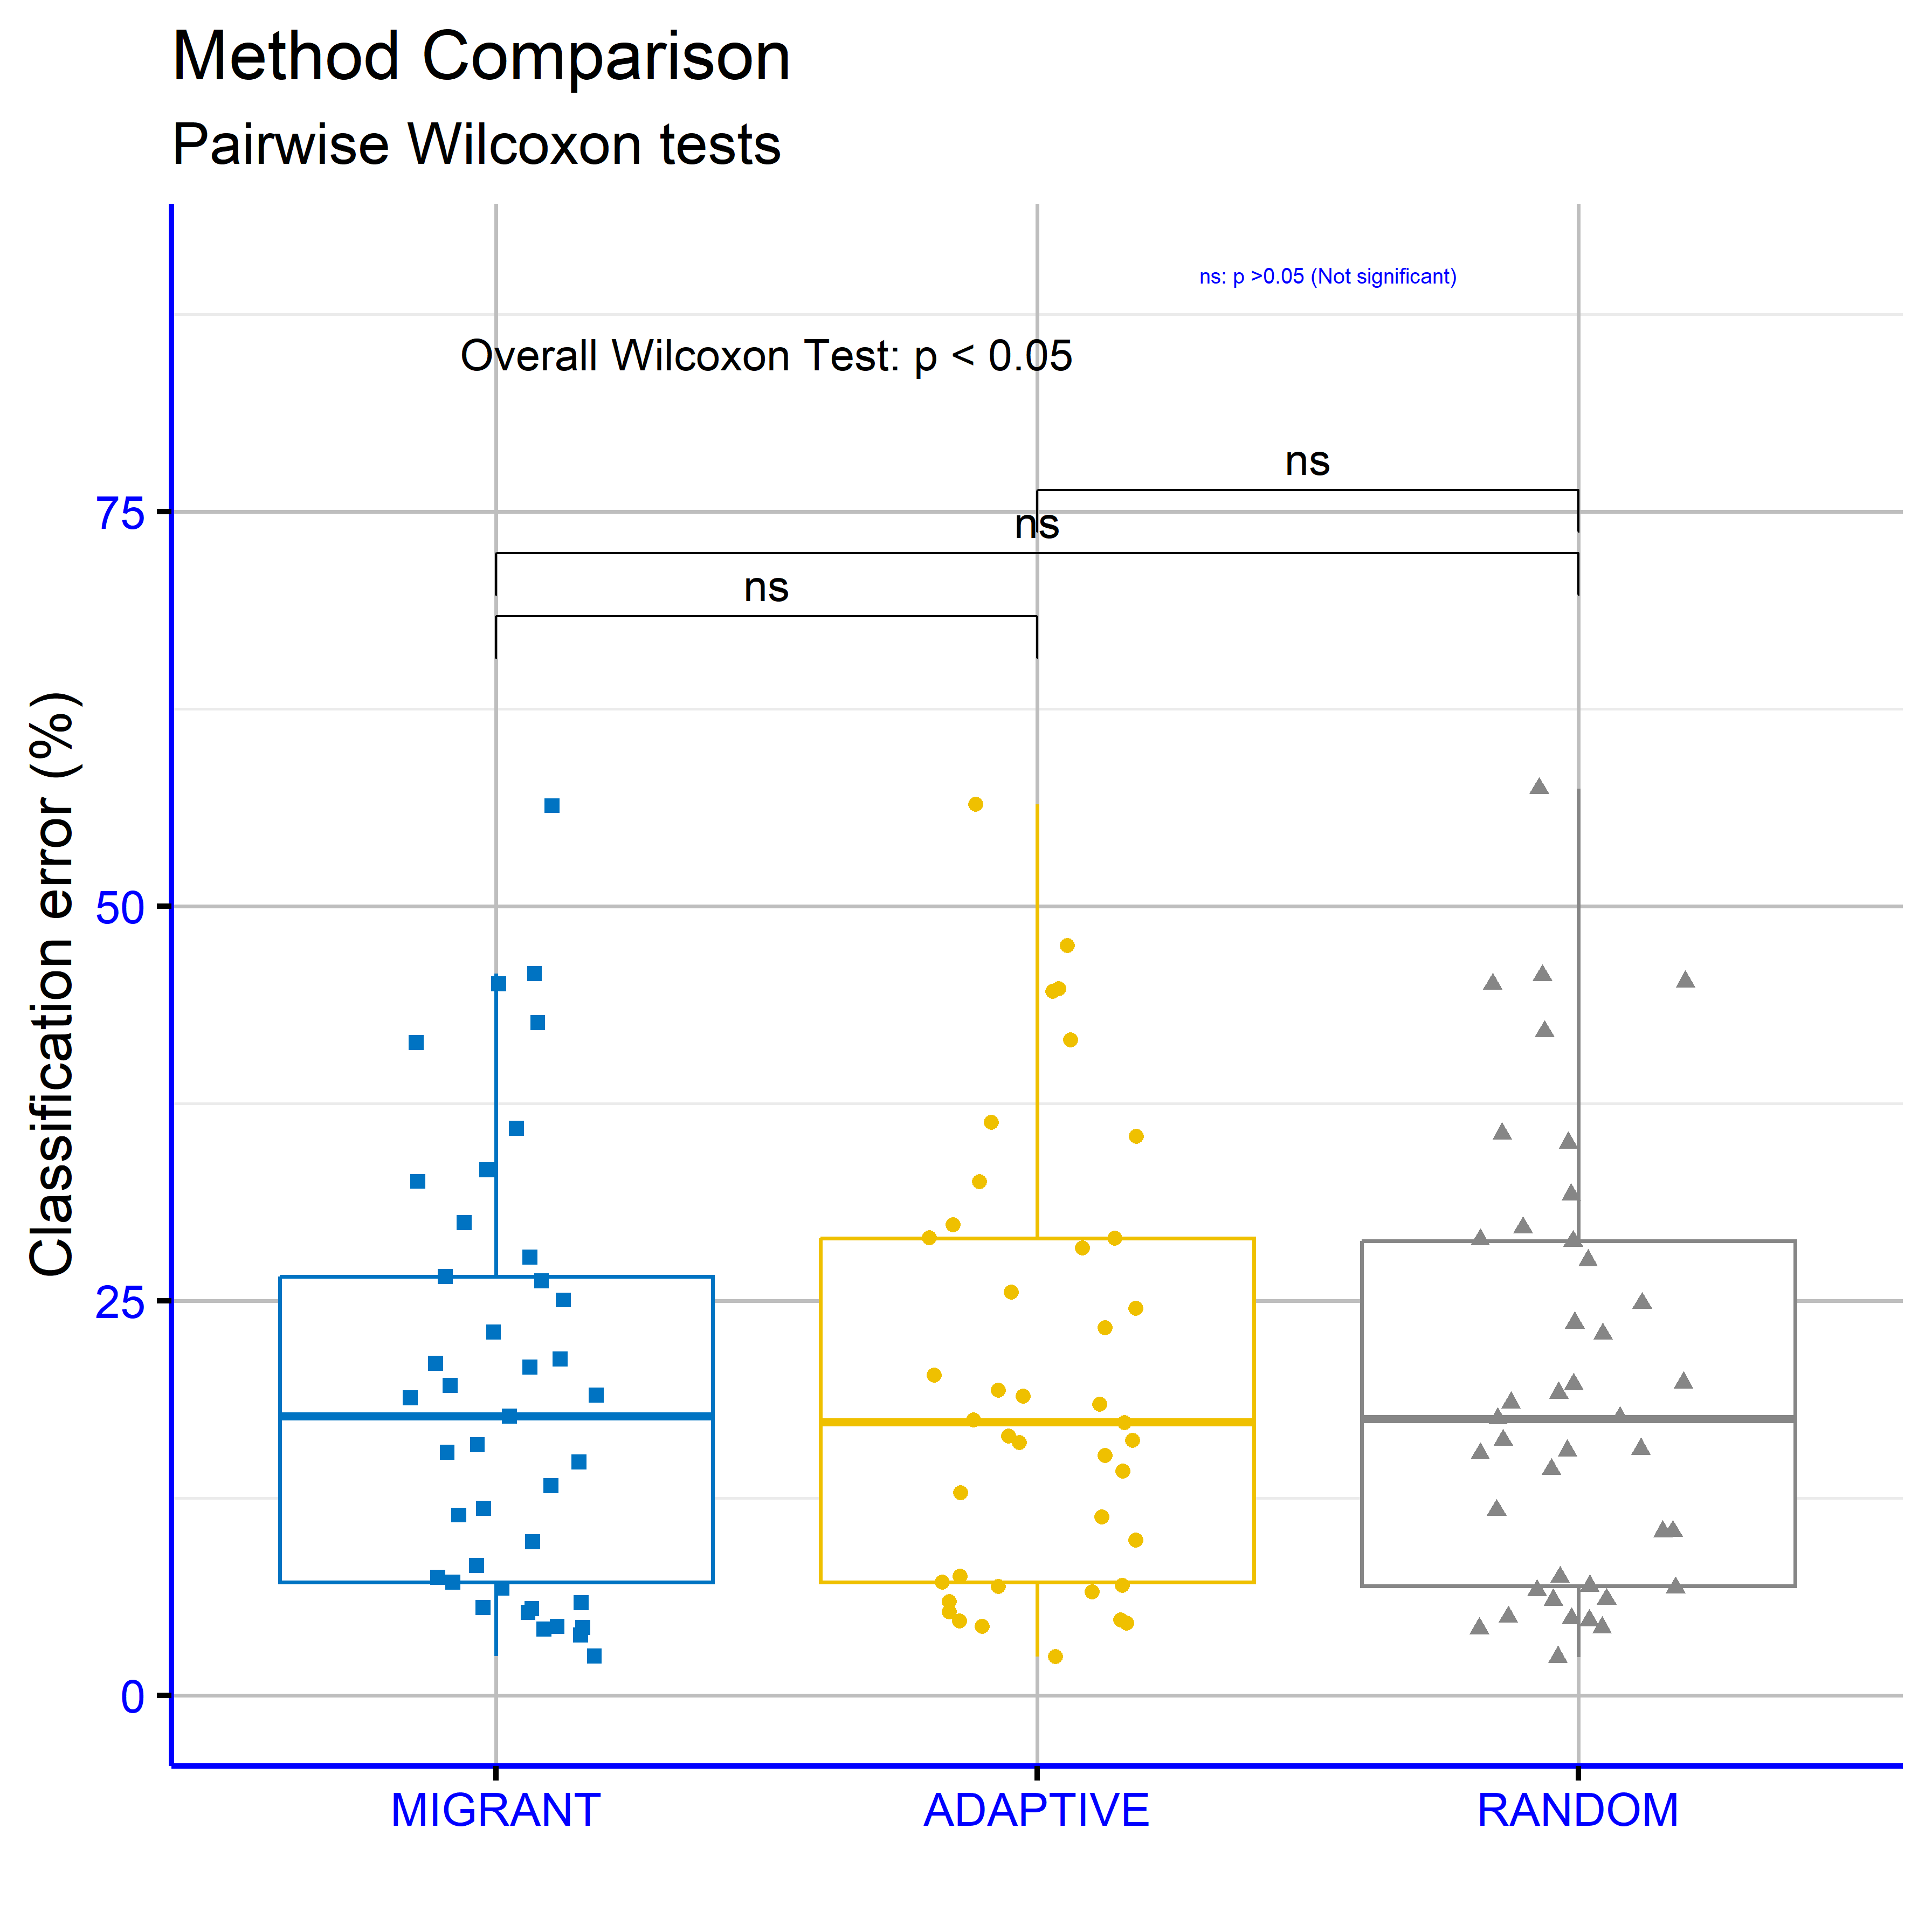
\includegraphics[scale=0.5]{s3}
\par\end{centering}
\caption{Statistical comparison for the obtained results on the classification
datasets using a series of differential weight mechanisms. \label{fig:statFclass}}

\end{figure}

An analysis was conducted to compare different methods for calculating
differential weight in the proposed machine learning approach on the
regression datasets. The Wilcoxon Test was used for pairwise comparisons,
applied across the series of regression datasets, with a focus on
regression error. The aim was to determine the statistical significance
of the observed differences between the methods Figure \ref{fig:statFRegression}.
The results showed that the comparison between MIGRANT and ADAPTIVE
yielded a p-value of 0.68, indicating no statistically significant
difference between these two methods. Similarly, the comparison between
MIGRANT and RANDOM resulted in a p-value of 0.9, confirming the absence
of a statistically significant difference in this case as well. However,
the comparison between ADAPTIVE and RANDOM produced a p-value of 0.00095,
which is below the standard threshold for statistical significance
(commonly 0.05). This suggests a statistically significant difference
between these two approaches. Overall, the findings indicate that
the MIGRANT and ADAPTIVE methods, as well as the MIGRANT and RANDOM
methods, exhibit similar performance regarding regression error. In
contrast, the ADAPTIVE method shows a clear and statistically significant
differentiation from the RANDOM method. 

\begin{figure}[H]
\begin{centering}
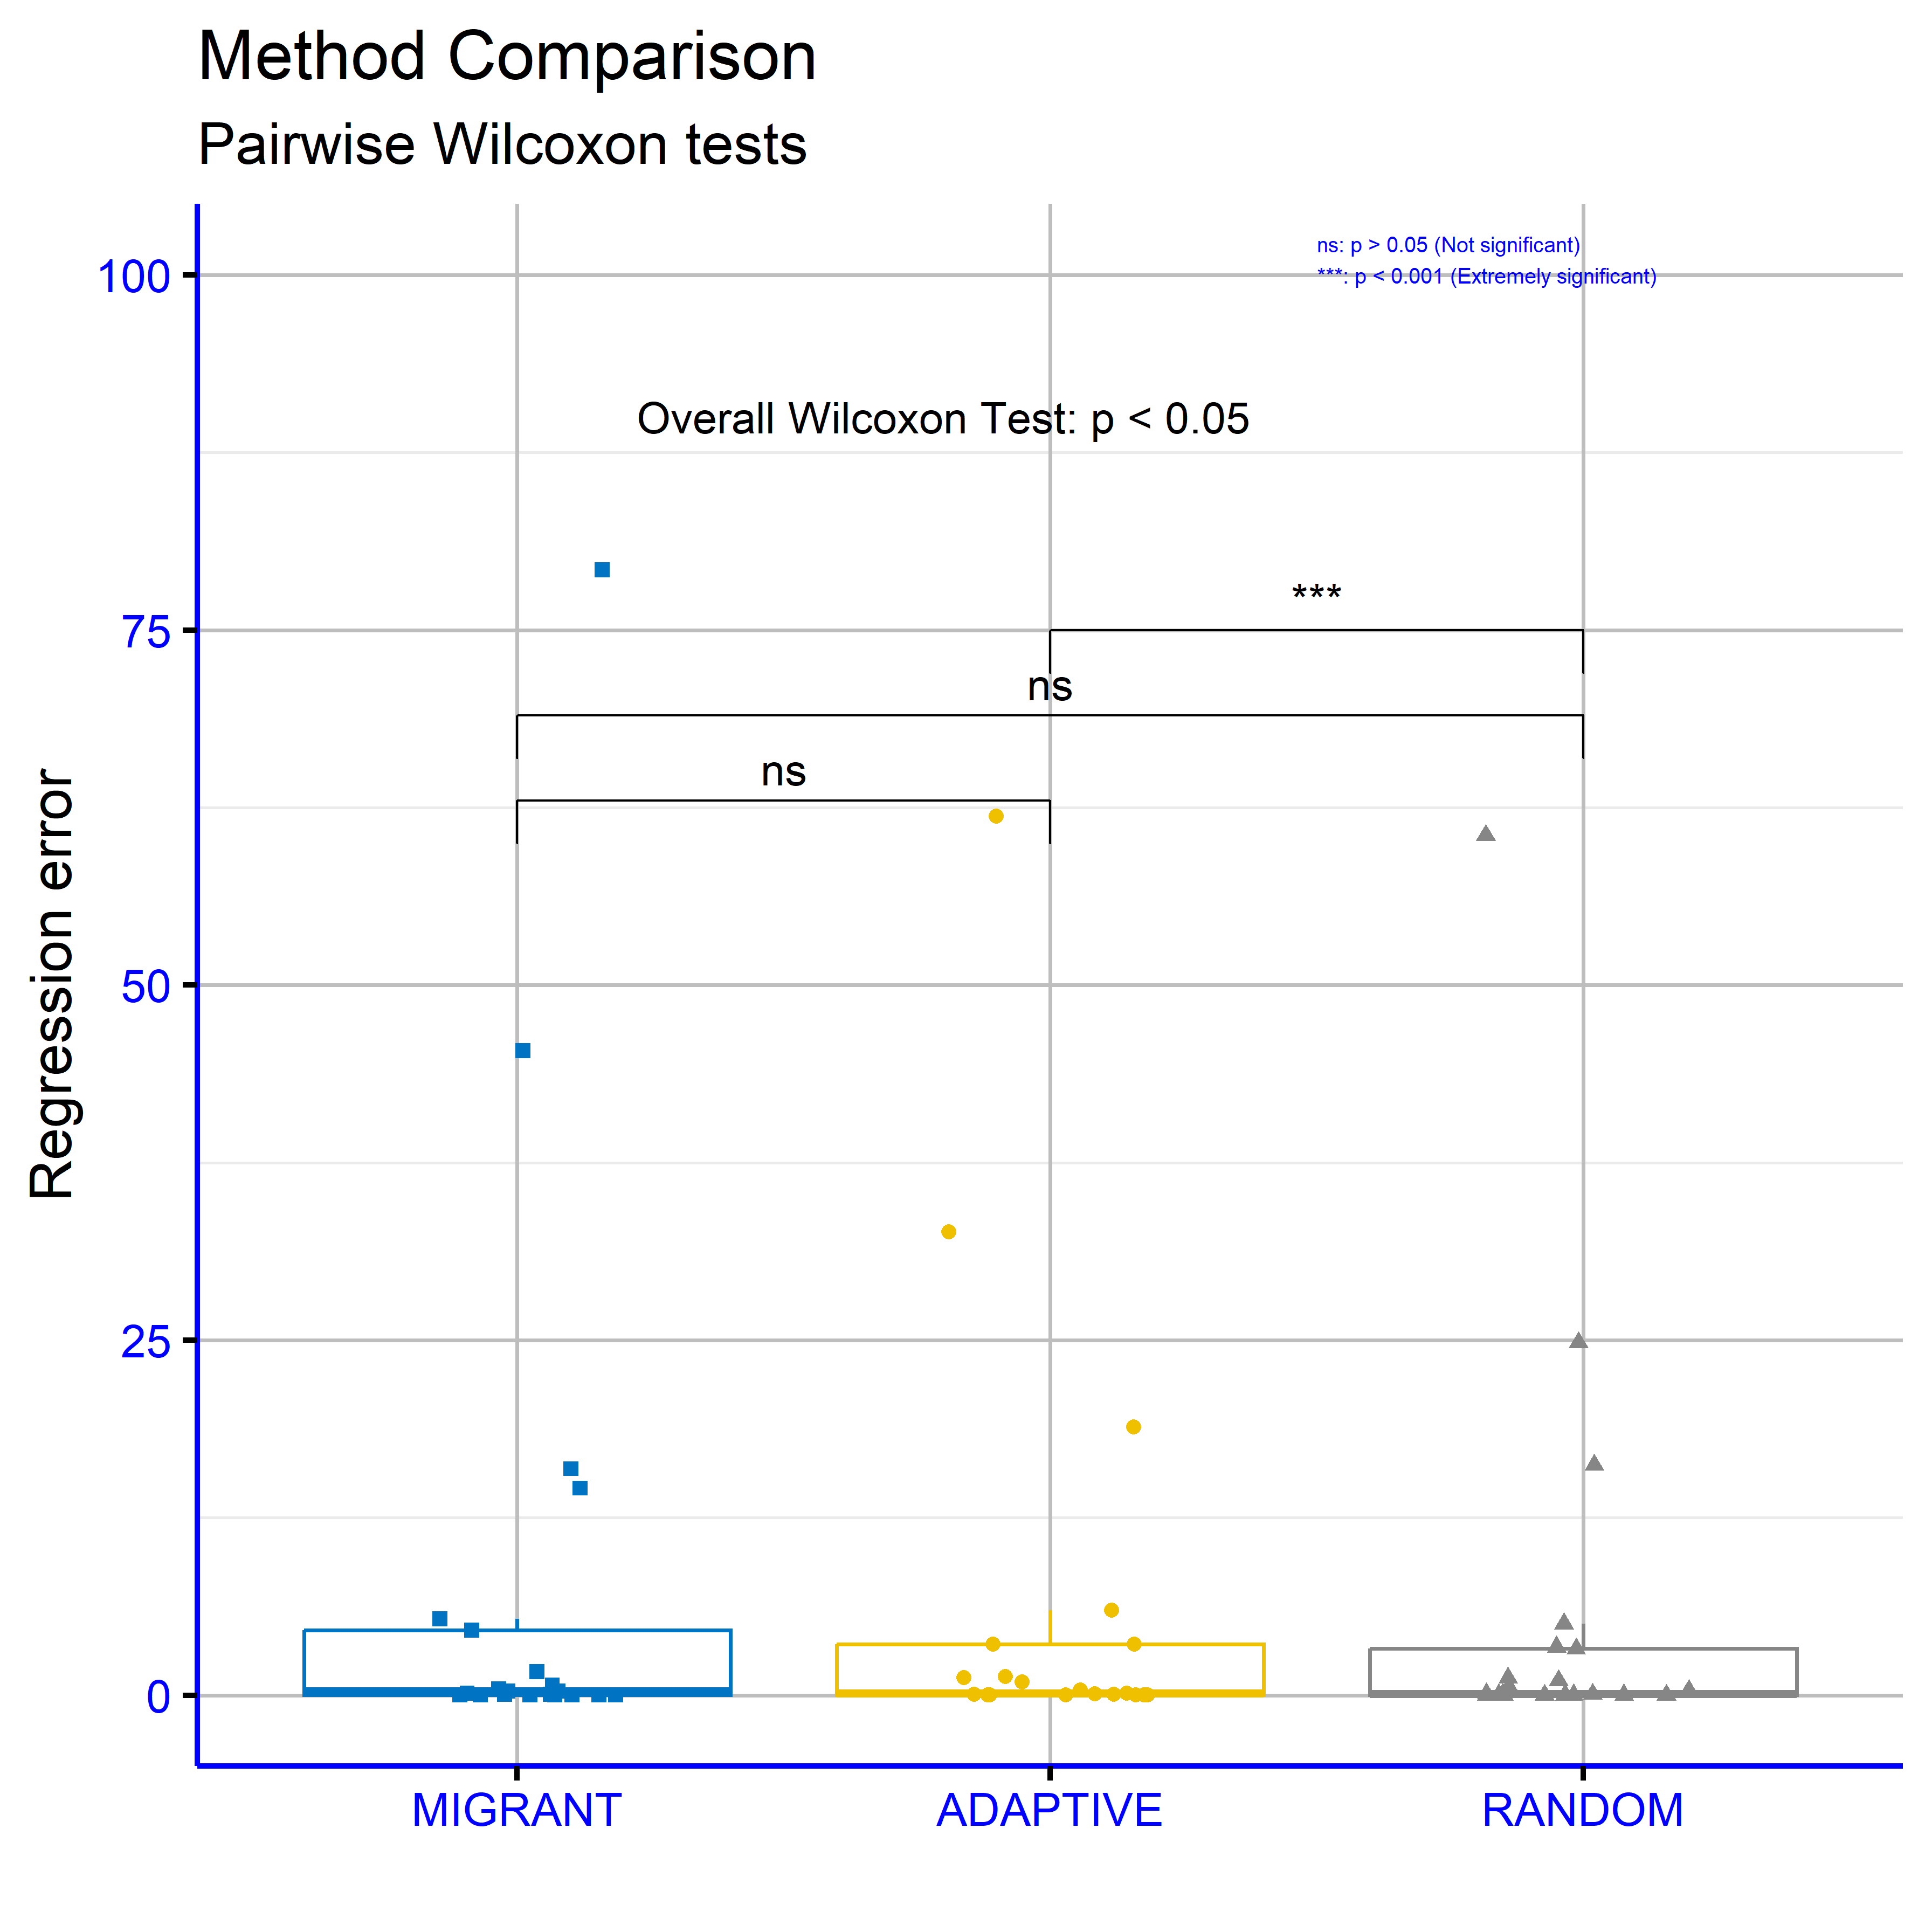
\includegraphics[scale=0.5]{s4}
\par\end{centering}
\caption{Statistical comparison between the various differential weight mechanisms
for the regression datasets.\label{fig:statFRegression}}

\end{figure}


\subsubsection{Experiments with the factor $a$ }

In the next series of experiments, the effect of the parameter $a$
on the behavior of the method on classification and data fitting data
was studied. In this series of experiments, different values of this
parameter were studied. This parameter determines the allowable range
of values within which the local minimization method can vary the
parameters of the artificial neural network.

The Table \ref{tab:experAClass} presents error percentages across
the used classification datasets for different values of the parameter
$a$ (1.25, 1.5, 2, 4, and 8). The lowest overall average error is
observed for $a=2$ with an average of 19.78\%. This suggests that
$a=2$ provides the most balanced performance across datasets. The
other parameter values---1.25, 1.5, 4, and 8---yield average errors
of 19.98\%, 19.95\%, 20.00\%, and 19.95\%, respectively. These results
indicate that $a=2$ has a slight advantage in minimizing the overall
error compared to other values. For individual datasets, the performance
varies depending on the parameter value. For example, in the ALCOHOL
dataset, the smallest error is achieved at $a=2$ with 19.15\%, while
other values result in slightly higher errors. Similarly, in the SEGMENT
dataset, the error is minimized at $a=8$ with 14.27\%. However, in
datasets like SPIRAL, the errors across all parameter values are close,
with no significant advantage for any specific value. In certain datasets,
there is a clear trend in error reduction as the parameter value changes.
For example, in the SEGMENT dataset, errors decrease consistently
from $a=1.25$ to $a=8$. Conversely, in the ZOO dataset, the error
decreases for lower values of a but increases again at higher values,
indicating that performance is not always linear with changes in $a$.
Some datasets exhibit minimal variability in performance across parameter
values. For example, the error for the LIVERDISORDER dataset remains
relatively stable, ranging from 31.41\% to 32.33\%. Similarly, the
SPIRAL dataset shows little variation, with errors consistently around
42\%. In other cases, specific parameter values consistently underperform.
For instance, in the Z\_F\_S dataset, $a=1.5$ achieves the lowest
error of 6.67\%, while $a=2$ and $a=4$ result in slightly higher
errors. Similarly, $a=8$ achieves the smallest error for certain
datasets like SEGMENT but performs poorly for datasets like WINE.
Overall, $a=2$ emerges as the most effective parameter value, yielding
the smallest average error across datasets. While other values of
$a$ perform well in individual cases, their overall performance is
less consistent. 

\begin{table}[H]
\caption{Experimental results for the classification datasets using different
values for the critical parameter $a$. In each column a different
value for the critical parameter is used and numbers in cells represent
the average classification error.\label{tab:experAClass}}

\centering{}%
\begin{tabular}{|c|c|c|c|c|c|}
\hline 
DATASET & $a=1.25$ & $a=1.5$ & $a=2$ & $a=4$ & $a=8$\tabularnewline
\hline 
\hline 
ALCOHOL & 21.49\% & 20.20\% & 19.15\% & 22.34\% & 19.86\%\tabularnewline
\hline 
AUSTRALIAN & 16.43\% & 16.89\% & 15.31\% & 15.90\% & 16.16\%\tabularnewline
\hline 
BALANCE & 7.49\% & 7.56\% & 6.92\% & 7.01\% & 7.16\%\tabularnewline
\hline 
BANDS & 34.88\% & 35.09\% & 35.00\% & 35.61\% & 35.01\%\tabularnewline
\hline 
CLEVELAND & 44.86\% & 46.08\% & 45.07\% & 44.67\% & 45.07\%\tabularnewline
\hline 
CIRCULAR & 4.17\% & 4.26\% & 4.23\% & 4.49\% & 4.61\%\tabularnewline
\hline 
DERMATOLOGY & 10.77\% & 10.65\% & 10.38\% & 9.87\% & 8.94\%\tabularnewline
\hline 
ECOLI & 44.13\% & 45.87\% & 45.22\% & 46.65\% & 47.46\%\tabularnewline
\hline 
HABERMAN & 27.24\% & 27.02\% & 27.55\% & 27.91\% & 28.40\%\tabularnewline
\hline 
HAYES-ROTH & 36.95\% & 36.46\% & 35.59\% & 35.82\% & 33.21\%\tabularnewline
\hline 
HEART & 17.43\% & 17.17\% & 17.60\% & 17.19\% & 17.19\%\tabularnewline
\hline 
HEARTATTACK & 19.50\% & 19.27\% & 19.70\% & 19.69\% & 19.69\%\tabularnewline
\hline 
HEPATITIS & 59.00\% & 57.38\% & 57.46\% & 60.21\% & 60.96\%\tabularnewline
\hline 
HOUSEVOTES & 7.07\% & 7.90\% & 7.48\% & 7.06\% & 7.07\%\tabularnewline
\hline 
IONOSPHERE & 14.24\% & 15.48\% & 16.17\% & 16.17\% & 15.43\%\tabularnewline
\hline 
LIVERDISORDER & 31.41\% & 31.59\% & 31.72\% & 32.23\% & 32.33\%\tabularnewline
\hline 
LYMOGRAPHY & 27.00\% & 27.07\% & 28.86\% & 27.57\% & 27.09\%\tabularnewline
\hline 
MAGIC & 12.18\% & 11.94\% & 11.73\% & 11.78\% & 12.25\%\tabularnewline
\hline 
MAMMOGRAPHIC & 17.42\% & 17.46\% & 17.52\% & 17.56\% & 17.54\%\tabularnewline
\hline 
PARKINSONS & 13.67\% & 13.40\% & 14.32\% & 14.19\% & 13.83\%\tabularnewline
\hline 
PAGE BLOCKS & 6.32\% & 6.28\% & 6.04\% & 5.83\% & 5.92\%\tabularnewline
\hline 
PHONEME & 16.07\% & 15.69\% & 15.50\% & 15.00\% & 15.00\%\tabularnewline
\hline 
PIMA & 24.59\% & 24.61\% & 24.85\% & 24.57\% & 24.79\%\tabularnewline
\hline 
POPFAILURES & 4.90\% & 5.28\% & 6.09\% & 7.50\% & 6.94\%\tabularnewline
\hline 
REGIONS2 & 29.35\% & 28.94\% & 28.77\% & 28.79\% & 28.69\%\tabularnewline
\hline 
RING & 27.65\% & 26.97\% & 22.90\% & 23.92\% & 23.20\%\tabularnewline
\hline 
SAHEART & 29.33\% & 29.37\% & 29.63\% & 29.97\% & 30.47\%\tabularnewline
\hline 
SEGMENT & 18.18\% & 16.86\% & 15.60\% & 14.53\% & 14.27\%\tabularnewline
\hline 
SONAR & 19.27\% & 19.62\% & 19.80\% & 18.87\% & 20.16\%\tabularnewline
\hline 
SPAMBASE & 4.67\% & 5.07\% & 4.95\% & 5.00\% & 5.87\%\tabularnewline
\hline 
SPIRAL & 41.92\% & 41.76\% & 42.06\% & 41.49\% & 42.13\%\tabularnewline
\hline 
STATHEART & 19.22\% & 18.91\% & 18.53\% & 19.30\% & 20.22\%\tabularnewline
\hline 
STUDENT & 4.76\% & 4.55\% & 4.86\% & 5.84\% & 6.43\%\tabularnewline
\hline 
TAE & 47.54\% & 46.22\% & 45.62\% & 46.07\% & 44.38\%\tabularnewline
\hline 
TRANSFUSION & 23.74\% & 23.87\% & 23.59\% & 23.95\% & 24.15\%\tabularnewline
\hline 
WDBC & 4.48\% & 4.50\% & 4.29\% & 4.12\% & 4.14\%\tabularnewline
\hline 
WINE & 9.24\% & 9.67\% & 10.39\% & 10.39\% & 11.88\%\tabularnewline
\hline 
Z\_F\_S & 7.26\% & 6.67\% & 6.81\% & 6.64\% & 6.70\%\tabularnewline
\hline 
ZO\_NF\_S & 4.82\% & 4.91\% & 4.73\% & 4.42\% & 4.33\%\tabularnewline
\hline 
ZONF\_S & 2.42\% & 2.55\% & 2.41\% & 2.68\% & 2.60\%\tabularnewline
\hline 
ZOO & 6.23\% & 6.93\% & 6.63\% & 7.07\% & 6.40\%\tabularnewline
\hline 
\textbf{AVERAGE} & \textbf{19.98\%} & \textbf{19.95\%} & \textbf{19.78\%} & \textbf{20.00\%} & \textbf{19.95\%}\tabularnewline
\hline 
\end{tabular}
\end{table}

The Table \ref{tab:experARegression} presents error rates for the
regression datasets across different values of the critical parameter
$a$ (1.25, 1.5, 2, 4, and 8). The lowest average error is observed
for $a=1.5$, with an average of 5.39, suggesting it offers the best
overall performance. $a=1.25$ ranks second with an average of 5.46,
and $a=2$ slightly higher at 5.56. The values $a=4$ and $a=8$ show
a marked increase in errors, with averages of 5.94 and 7.44, respectively.
This indicates that higher values of $a$ are less effective compared
to smaller ones. For individual datasets, performance varies with
the value of $a$. For instance, in the AIRFOIL dataset, the error
consistently decreases as $a$ increases, with the smallest error
(0.0007) observed at $a=8$. Conversely, in the FRIEDMAN dataset,
the error rises sharply at $a=8$ (19.74), signaling a significant
performance decline. In some datasets, such as BASEBALL, the error
steadily increases with higher values of $a$ rising from 57.67 at
a=1.25 to 72.37 at $a=8$. In contrast, in the HOUSING dataset, the
smallest error occurs at $a=4$ (22.86), although larger values like
$a=8$ show only a slight increase. Certain datasets exhibit minimal
sensitivity to changes in $a$. For example, in the LASER dataset,
errors remain almost constant regardless of the parameter value, ranging
from 0.0025 to 0.0035. Similarly, in the DEE dataset, the errors are
nearly identical across all values of $a$ showing minimal variation.
Interestingly, the PLASTIC dataset shows a gradual decrease in error
from 3.37 at a=1.25 to 2.8 at a=8, indicating improved performance
with increasing $a$. Conversely, in the STOCK dataset, the error
increases significantly from 2.82 at a=1.25 to 5.42 at $a=8$. In
conclusion, $a=1.5$ emerges as the optimal choice for minimizing
overall error in this analysis. Higher values of $a$ demonstrate
reduced effectiveness, especially at $a=8$, where the average error
rises notably. However, the results reveal that the impact of $a$
varies by dataset, with some benefiting from smaller values and others
exhibiting relative insensitivity to parameter changes. 

\begin{table}[H]
\caption{Experimental results for the regression datasets using different values
for the critical parameter $a$. Each column contains experiments
with different values for the critical parameter $a$. The numbers
in cells represent average regression error for the corresponding
test set.\label{tab:experARegression}}

\centering{}%
\begin{tabular}{|c|c|c|c|c|c|}
\hline 
DATASET & $a=1.25$ & $a=1.5$ & $a=2$ & $a=4$ & $a=8$\tabularnewline
\hline 
\hline 
ABALONE & 4.36 & 4.66 & 5.04 & 7.63 & 8.84\tabularnewline
\hline 
AIRFOIL & 0.002 & 0.0018 & 0.0014 & 0.0009 & 0.0007\tabularnewline
\hline 
AUTO & 14.97 & 14.72 & 16.21 & 16.04 & 16.58\tabularnewline
\hline 
BK & 0.02 & 0.02 & 0.019 & 0.11 & 0.21\tabularnewline
\hline 
BL & 0.011 & 0.012 & 0.016 & 0.037 & 0.11\tabularnewline
\hline 
BASEBALL & 57.67 & 58.42 & 60.56 & 67.70 & 72.37\tabularnewline
\hline 
CONCRETE & 0.003 & 0.003 & 0.003 & 0.004 & 0.005\tabularnewline
\hline 
DEE & 0.35 & 0.34 & 0.35 & 0.34 & 0.34\tabularnewline
\hline 
FA & 0.067 & 0.056 & 0.083 & 0.24 & 0.42\tabularnewline
\hline 
FRIEDMAN & 1.30 & 1.24 & 1.22 & 1.41 & 19.74\tabularnewline
\hline 
HO & 0.011 & 0.012 & 0.017 & 0.043 & 0.17\tabularnewline
\hline 
HOUSING & 28.09 & 25.93 & 24.82 & 22.86 & 26.45\tabularnewline
\hline 
LASER & 0.0026 & 0.0025 & 0.0026 & 0.0027 & 0.0035\tabularnewline
\hline 
LW & 0.019 & 0.019 & 0.021 & 0.073 & 0.77\tabularnewline
\hline 
MORTGAGE & 0.50 & 0.45 & 0.54 & 0.75 & 0.62\tabularnewline
\hline 
PLASTIC & 3.37 & 3.10 & 3.27 & 3.02 & 2.80\tabularnewline
\hline 
PY & 0.12 & 0.13 & 0.11 & 0.09 & 0.09\tabularnewline
\hline 
QUAKE & 0.04 & 0.041 & 0.042 & 0.048 & 0.096\tabularnewline
\hline 
SN & 0.024 & 0.024 & 0.027 & 0.087 & 0.17\tabularnewline
\hline 
STOCK & 2.82 & 3.13 & 3.40 & 3.21 & 5.42\tabularnewline
\hline 
TREASURY & 0.87 & 0.81 & 1.021 & 1.06 & 1.06\tabularnewline
\hline 
\textbf{AVERAGE} & \textbf{5.46} & \textbf{5.39} & \textbf{5.56} & \textbf{5.94} & \textbf{7.44}\tabularnewline
\hline 
\end{tabular}
\end{table}

In Figure \ref{fig:statAClass}, a comparison of various values of
the parameter $a$ which defines the bounds of optimal values in the
proposed machine learning method, is presented. The comparisons were
conducted using the Wilcoxon Test across the series of used datasets
to evaluate the classification error. The results indicate that the
p-values for all pairwise comparisons between different values of
$a$ are above the significance level of 0.05, suggesting no statistically
significant differences. For instance, comparisons between $a=1.25$
and other values (1.5, 2, 4, 8) yielded p-values ranging from 0.6
to 0.73, while comparisons between $a=1.5$ and other values (2, 4,
8) produced p-values ranging from 0.32 to 0.8. Similarly, comparisons
between $a=2$ and higher values (4 and 8) resulted in p-values of
0.22 and 0.31, respectively, whereas the comparison between $a=4$
and $a=8$ yielded a p-value of 0.69. In conclusion, the results suggest
that variations in the parameter $a$ within the specified range do
not lead to statistically significant differences in classification
error, as all p-values remain well above the conventional significance
threshold. Therefore, the choice of a specific value for $a$ is likely
to have little or no impact on the method's performance, based on
the current data.

\begin{figure}[H]
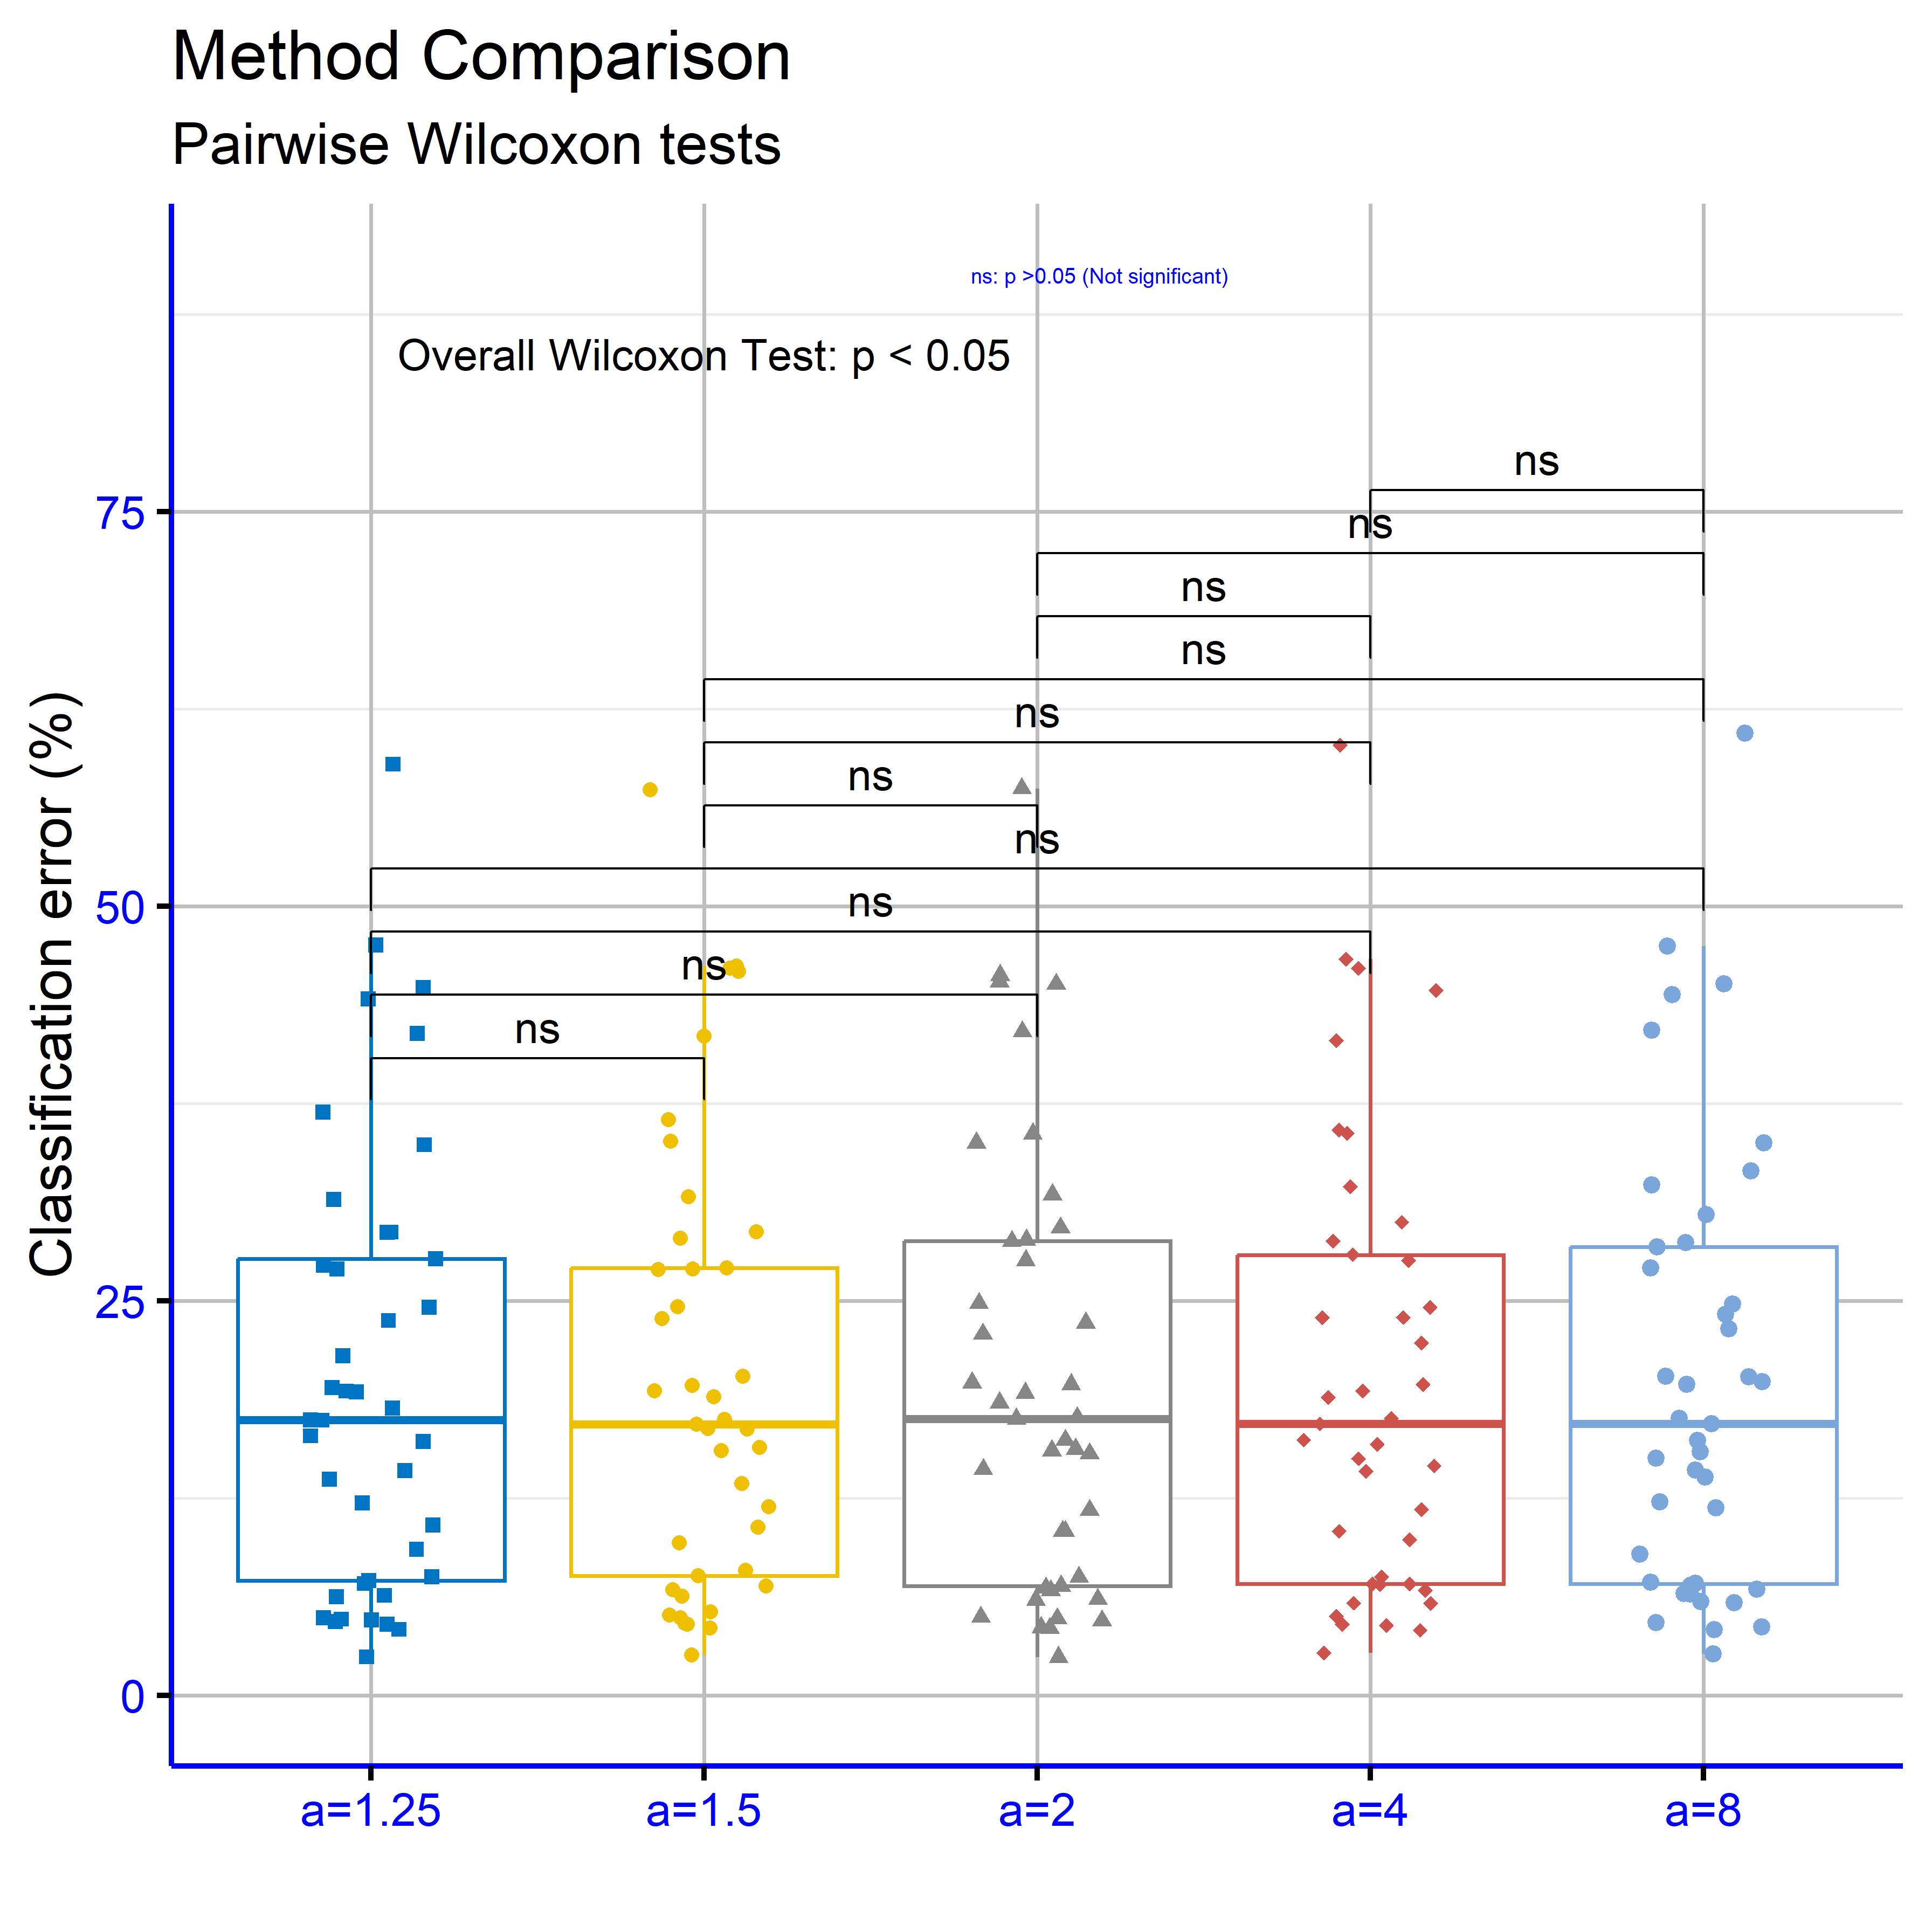
\includegraphics[scale=0.5]{s5}

\caption{Statistical comparison for the experiments with different values for
the parameter $a$. The method was applied on the classification datasets.\label{fig:statAClass}}

\end{figure}

In Figure \ref{fig:statARegression}, the comparison of different
values of parameter $a$ for the regression error is presented. The
results showed that statistically significant differences were observed
in some comparisons, as the p-values were below the significance level
of 0.05. For example, the comparison between $a=1.25$ and $a=4$
yielded p=0.024, while between $a=1.25$ and $a=8$, p=0.017 was observed.
Similarly, the comparison between $a=1.5$ and $a=8$ resulted in
p=0.0021, indicating strong statistical significance. Conversely,
some comparisons did not show statistically significant differences,
as the p-values were above the significance level. For instance, the
comparison between $a=2$ and $a=4$ yielded p=0.22, while the comparison
between $a=1.25$ and $a=2$ resulted in p=0.15. In conclusion, the
results suggest that the choice of parameter $a$ affects the regression
error in certain cases, with statistically significant differences
primarily observed in comparisons between smaller and larger values
of the parameter. However, the differences are not always consistent
and depend on the specific combinations of values being compared.

\begin{figure}[H]
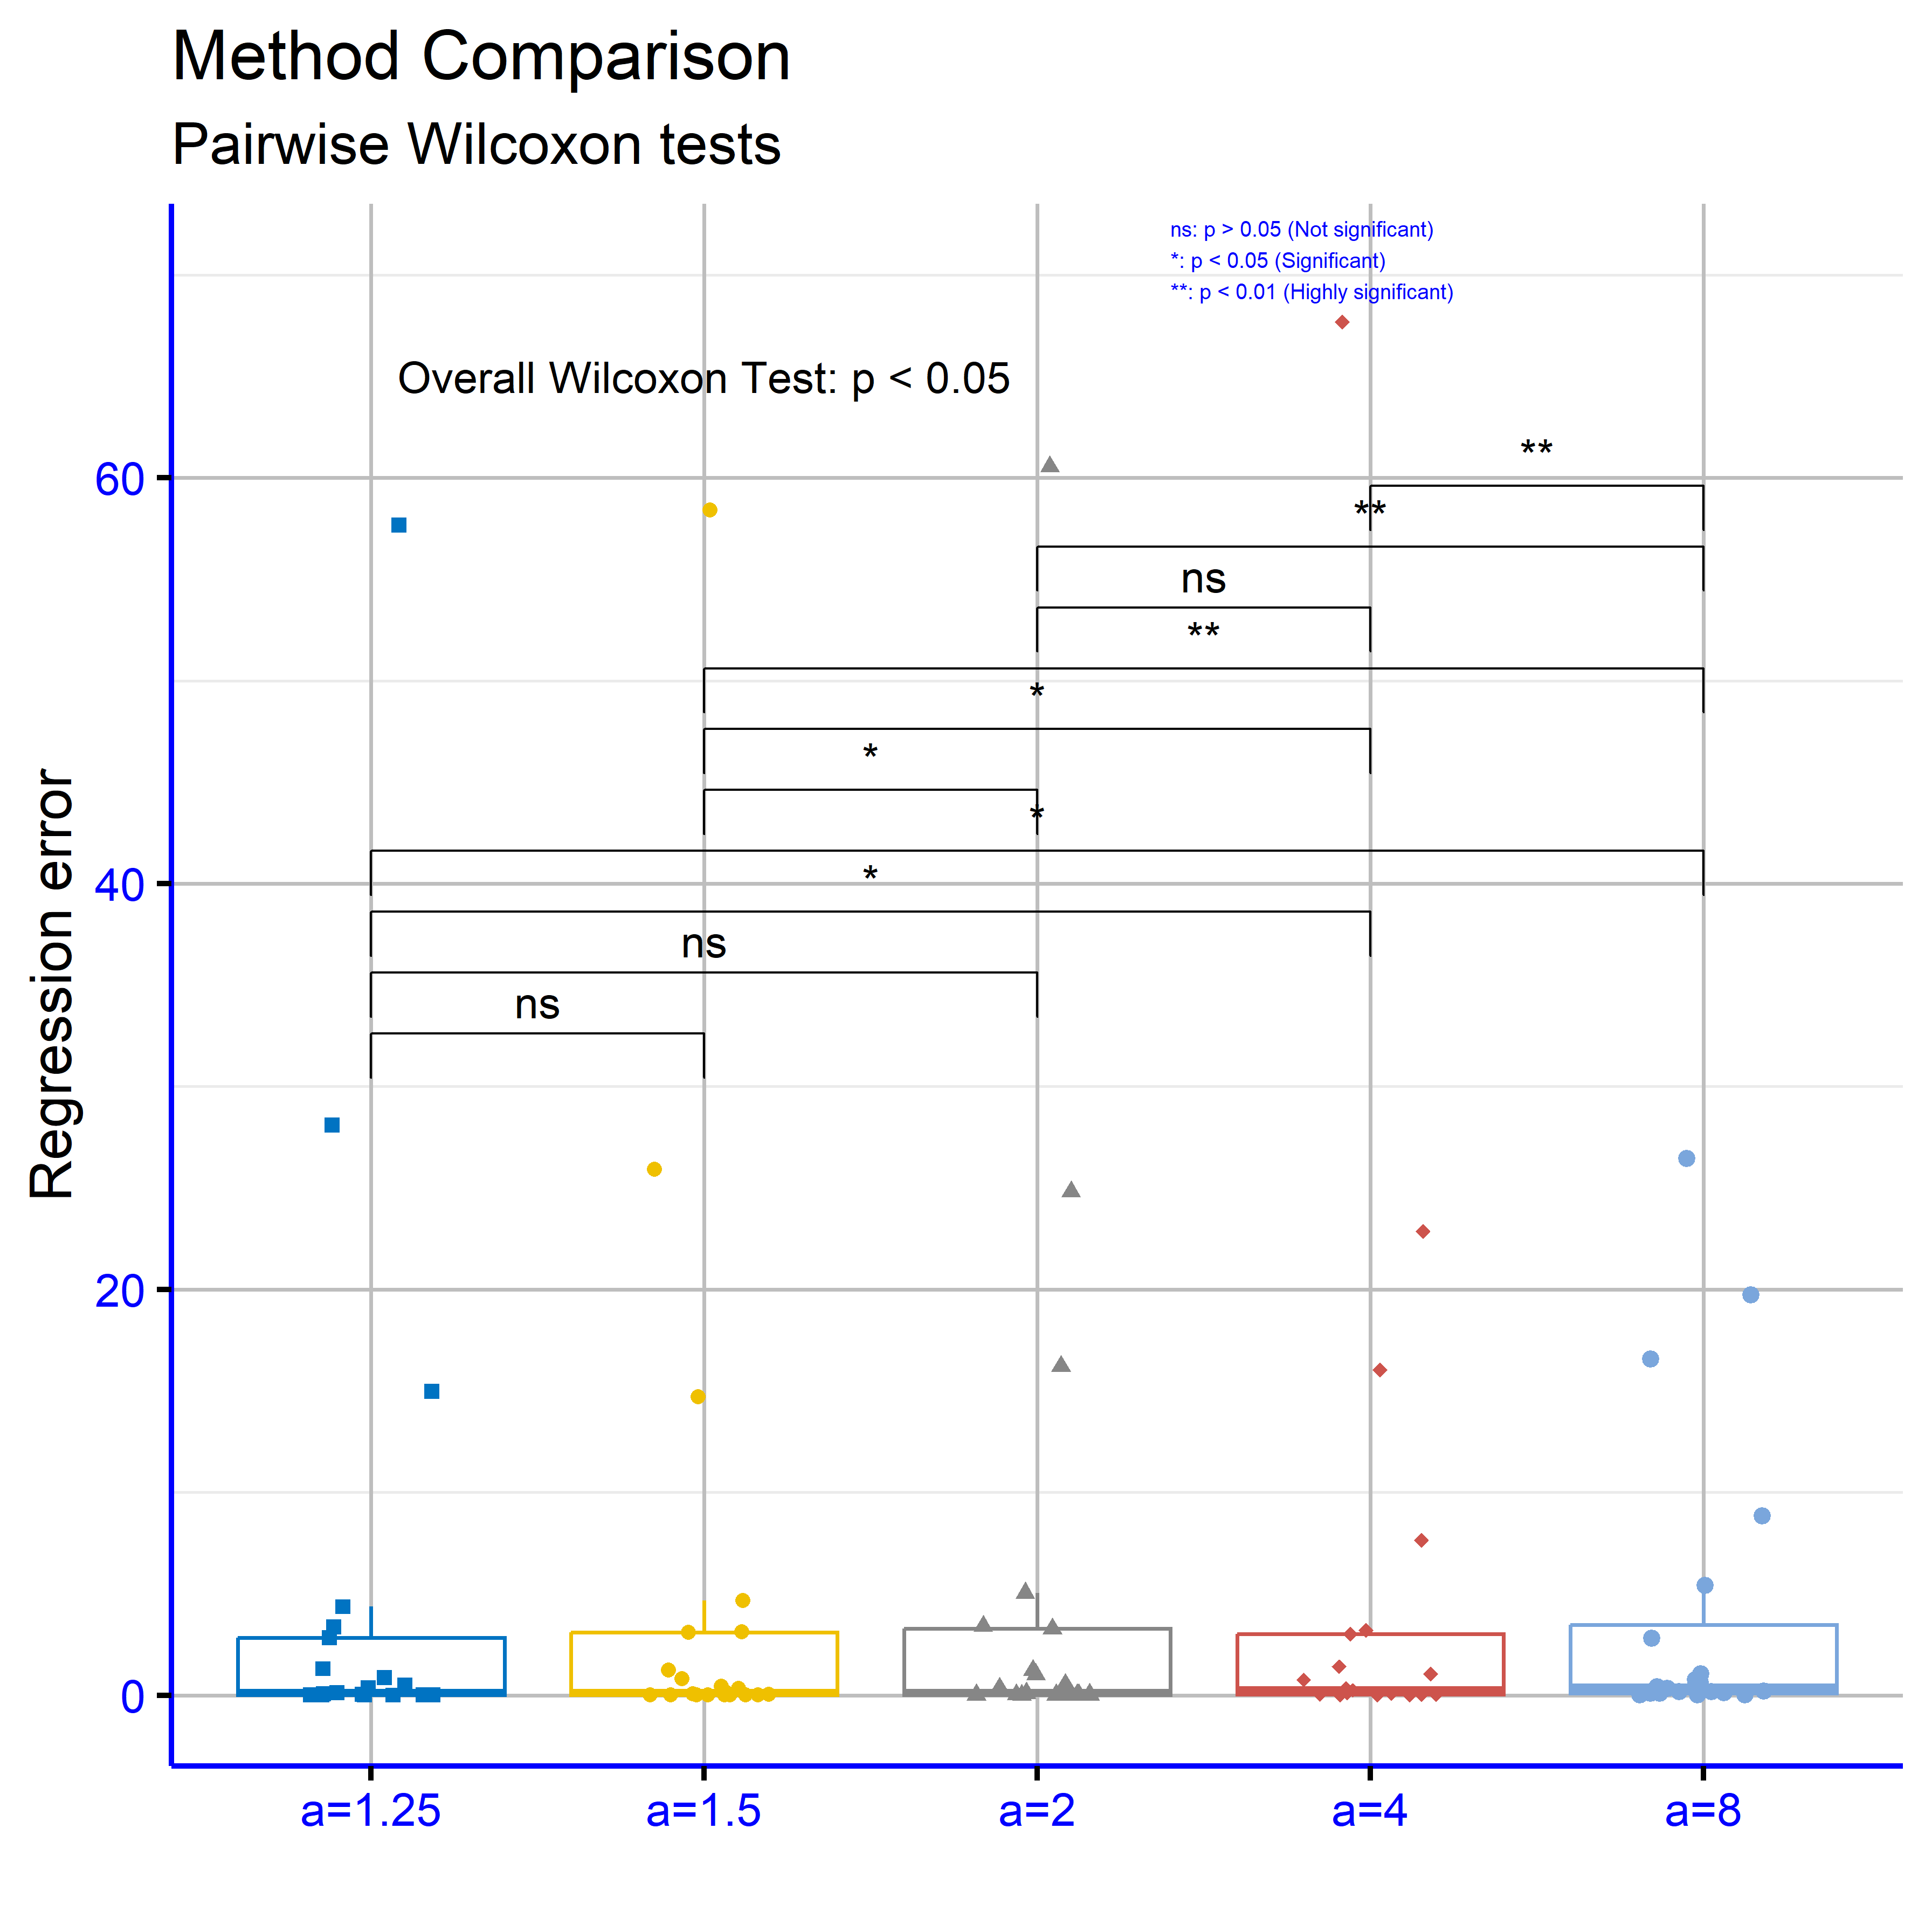
\includegraphics[scale=0.5]{s6}

\caption{Statistical comparison for the experiments using different values
for the parameter $a$. The method was applied on the regression datasets.\label{fig:statARegression}}

\end{figure}


\subsubsection{Experiments with the local search rate}

In the last series of experiments, the effect of the execution rate
of local optimization methods was studied. For this reason, values
ranging from 0.25\% to 2\% were studied.

The Table \ref{tab:experPLClass} provides error rates for the used
classification datasets under different values of periodic local search
$p_{l}$ (0.0025, 0.005, 0.01, and 0.02). The analysis reveals that
the lowest average error is observed $p_{l}=0.02$, with an error
rate of 19.43\%, suggesting that this value yields the best overall
performance. This is closely followed by $p_{l}=0.01$ with an average
error of 19.66\% and $p_{l}=0.005$ with 19.78\%. The highest average
error occurs at $p_{l}=0.0025$ with 20.48\%, indicating comparatively
poorer performance. Examining individual datasets, the impact of $p_{l}$
varies. For instance, in the ALCOHOL dataset, the smallest error is
observed at $p_{l}=0.02$ with 16.49\%, whereas larger values such
as $p_{l}=0.01$ and $p_{l}=0.005$ result in higher errors (21.81\%
and 19.15\%, respectively). Conversely, in the SEGMENT dataset, the
error consistently decreases as $p_{l}$ increases, reaching its lowest
value at $p_{l}=0.02$ with 11.70\%. This trend is also evident in
datasets such as SPAMBASE and WINE, where the errors decrease significantly
with higher $p_{l}$ values. Some datasets exhibit minimal sensitivity
to changes in $p_{l}$. For example, in the HEART and LIVERDISORDER
datasets, the error rates remain relatively stable across all $p_{l}$
values, showing only marginal fluctuations. In other cases, such as
CIRCULAR and HOUSEVOTES, the variations in error rates are similarly
minor. However, certain datasets show exceptions to the general trend.
For example, in the SONAR dataset, the error rate is lowest at $p_{l}=0.02$
with 18.53\%, but higher $p_{l}$ values like $p_{l}=0.01$ produce
increased errors (20.38\%). Similarly, the REGIONS2 dataset achieves
its best performance at $p_{l}=0.02$ with an error rate of 28.02\%,
but other $p_{l}$ values yield comparable results, such as 28.77\%
at both $p_{l}=0.005$ and $p_{l}=0.01$. The data suggests that higher
$p_{l}$ values, particularly $p_{l}=0.02$, generally result in improved
performance across most datasets. Nevertheless, the optimal $p_{l}$
value may vary depending on specific dataset characteristics, and
some datasets show negligible or inconsistent responses to changes
in $p_{l}$. Overall, $p_{l}=0.02$ is recommended for achieving the
lowest average error.

\begin{table}[H]
\caption{Experimental results for the classification datasets using different
values of local search rate $p_{l}$. In each column different value
for the local search rate is used. Numbers in cells stand for the
average classification error as measured on the corresponding test
set.\label{tab:experPLClass}}

\centering{}%
\begin{tabular}{|c|c|c|c|c|}
\hline 
DATASET & $p_{l}=0.0025$ & $p_{l}=0.005$ & $p_{l}=0.01$ & $p_{l}=0.02$\tabularnewline
\hline 
\hline 
ALCOHOL & 19.15\% & 19.15\% & 21.81\% & 16.49\%\tabularnewline
\hline 
AUSTRALIAN & 17.93\% & 15.31\% & 14.17\% & 14.14\%\tabularnewline
\hline 
BALANCE & 7.44\% & 6.92\% & 6.63\% & 6.54\%\tabularnewline
\hline 
BANDS & 35.66\% & 35.00\% & 35.01\% & 34.44\%\tabularnewline
\hline 
CLEVELAND & 46.45\% & 45.07\% & 45.39\% & 45.32\%\tabularnewline
\hline 
CIRCULAR & 4.21\% & 4.23\% & 4.16\% & 4.31\%\tabularnewline
\hline 
DERMATOLOGY & 11.25\% & 10.38\% & 9.96\% & 9.07\%\tabularnewline
\hline 
ECOLI & 46.64\% & 45.22\% & 44.34\% & 44.66\%\tabularnewline
\hline 
HABERMAN & 27.99\% & 27.55\% & 27.66\% & 27.43\%\tabularnewline
\hline 
HAYES-ROTH & 36.33\% & 35.59\% & 34.03\% & 31.44\%\tabularnewline
\hline 
HEART & 17.05\% & 17.60\% & 17.35\% & 17.51\%\tabularnewline
\hline 
HEARTATTACK & 19.62\% & 19.70\% & 19.43\% & 20.37\%\tabularnewline
\hline 
HEPATITIS & 60.13\% & 57.46\% & 58.79\% & 60.34\%\tabularnewline
\hline 
HOUSEVOTES & 7.81\% & 7.48\% & 8.02\% & 7.47\%\tabularnewline
\hline 
IONOSPHERE & 15.52\% & 16.17\% & 16.33\% & 16.72\%\tabularnewline
\hline 
LIVERDISORDER & 31.92\% & 31.72\% & 32.06\% & 32.40\%\tabularnewline
\hline 
LYMOGRAPHY & 27.48\% & 28.86\% & 29.55\% & 29.98\%\tabularnewline
\hline 
MAGIC & 12.00\% & 11.73\% & 11.55\% & 11.57\%\tabularnewline
\hline 
MAMMOGRAPHIC & 17.23\% & 17.52\% & 17.34\% & 17.57\%\tabularnewline
\hline 
PARKINSONS & 14.70\% & 14.32\% & 13.39\% & 14.04\%\tabularnewline
\hline 
PAGE BLOCKS & 6.02\% & 6.04\% & 5.66\% & 5.76\%\tabularnewline
\hline 
PHONEME & 15.67\% & 15.50\% & 15.29\% & 15.04\%\tabularnewline
\hline 
PIMA & 25.52\% & 24.85\% & 24.63\% & 24.87\%\tabularnewline
\hline 
POPFAILURES & 5.46\% & 6.09\% & 6.30\% & 6.75\%\tabularnewline
\hline 
REGIONS2 & 30.41\% & 28.77\% & 28.77\% & 28.02\%\tabularnewline
\hline 
RING & 27.01\% & 22.90\% & 24.05\% & 23.85\%\tabularnewline
\hline 
SAHEART & 29.91\% & 29.63\% & 29.54\% & 29.89\%\tabularnewline
\hline 
SEGMENT & 19.36\% & 15.60\% & 13.88\% & 11.70\%\tabularnewline
\hline 
SONAR & 19.62\% & 19.80\% & 20.38\% & 18.53\%\tabularnewline
\hline 
SPAMBASE & 6.30\% & 4.95\% & 5.43\% & 4.78\%\tabularnewline
\hline 
SPIRAL & 42.22\% & 42.06\% & 41.16\% & 40.35\%\tabularnewline
\hline 
STATHEART & 19.90\% & 18.53\% & 19.72\% & 20.47\%\tabularnewline
\hline 
STUDENT & 4.97\% & 4.86\% & 5.13\% & 5.01\%\tabularnewline
\hline 
TAE & 47.05\% & 45.62\% & 43.93\% & 45.05\%\tabularnewline
\hline 
TRANSFUSION & 24.41\% & 23.59\% & 23.11\% & 22.64\%\tabularnewline
\hline 
WDBC & 4.88\% & 4.29\% & 4.17\% & 4.07\%\tabularnewline
\hline 
WINE & 12.39\% & 10.39\% & 9.02\% & 8.41\%\tabularnewline
\hline 
Z\_F\_S & 7.11\% & 6.81\% & 6.26\% & 6.62\%\tabularnewline
\hline 
ZO\_NF\_S & 5.69\% & 4.73\% & 4.23\% & 3.93\%\tabularnewline
\hline 
ZONF\_S & 2.45\% & 2.41\% & 2.45\% & 2.38\%\tabularnewline
\hline 
ZOO & 6.93\% & 6.63\% & 6.00\% & 6.50\%\tabularnewline
\hline 
\textbf{AVERAGE} & \textbf{20.48\%} & \textbf{19.78\%} & \textbf{19.66\%} & \textbf{19.43\%}\tabularnewline
\hline 
\end{tabular}
\end{table}

The Table \ref{tab:experPlRegression} presents error rates for the
used regression datasets under different values of periodic local
search $p_{l}$ (0.0025, 0.005, 0.01, and 0.02). The analysis indicates
that the lowest average error is observed at $p_{l}=0.01$ with a
value of 5.04, suggesting that this setting offers the best overall
performance. This is followed by $p_{l}=0.02$ with an average error
of 5.10, $p_{l}=0.005$ with 5.56, and $p_{l}=0.0025$ with 6.34,
which has the highest average error and the poorest performance. Examining
individual datasets reveals variations in the impact of different
$p_{l}$ values. In the AUTO dataset, the error decreases steadily
as $p_{l}$ increases, dropping from 17.63 at $p_{l}=0.0025$ to its
lowest point of 10.11 at $p_{l}=0.02$. Similarly, in the HOUSING
dataset, the error significantly reduces from 32.72 at $p_{l}=0.0025$
to 14.02 at $p_{l}=0.02$. This decreasing trend is also evident in
other datasets, such as MORTGAGE, where the error falls from 1.22
at $p_{l}=0.0025$ to just 0.032 at $p_{l}=0.02$, and STOCK, where
the error reduces from 6.58 to 1.47. In some datasets, the $p_{l}$
parameter has minimal impact. For instance, in the CONCRETE dataset,
the error remains constant across all $p_{l}$ values at 0.003. Similar
stability is observed in the QUAKE and SN datasets, where variations
are minimal. However, some datasets exhibit less predictable trends.
In the BASEBALL dataset, the error initially decreases from 63.05
at $p_{l}=0.0025$ to 60.56 at $p_{l}=0.005$, but then increases
again to 71.93 at $p_{l}=0.02$. Similar inconsistent results are
observed in the PY and BL datasets. Overall, the analysis suggests
that $p_{l}=0.01$ delivers the best average performance. Nevertheless,
the effect of the $p_{l}$ parameter varies across datasets, with
some benefiting more from higher or lower $p_{l}$ values. 

\begin{table}[H]
\caption{Experimental results for the regression datasets using different values
of the local search rate parameter $p_{l}$. The columns contain experiments
with different values of the local search rate and numbers in cells
represent average regression error for the corresponding test set.\label{tab:experPlRegression}}

\centering{}%
\begin{tabular}{|c|c|c|c|c|}
\hline 
DATASET & $p_{l}=0.0025$ & $p_{l}=0.005$ & $p_{l}=0.01$ & $p_{l}=0.02$\tabularnewline
\hline 
\hline 
ABALONE & 4.48 & 5.04 & 5.27 & 4.93\tabularnewline
\hline 
AIRFOIL & 0.0019 & 0.0014 & 0.0009 & 0.0006\tabularnewline
\hline 
AUTO & 17.63 & 16.21 & 12.50 & 10.11\tabularnewline
\hline 
BK & 0.027 & 0.019 & 0.03 & 0.029\tabularnewline
\hline 
BL & 0.031 & 0.016 & 0.05 & 0.017\tabularnewline
\hline 
BASEBALL & 63.05 & 60.56 & 62.57 & 71.93\tabularnewline
\hline 
CONCRETE & 0.003 & 0.003 & 0.003 & 0.003\tabularnewline
\hline 
DEE & 0.36 & 0.35 & 0.32 & 0.31\tabularnewline
\hline 
FA & 0.056 & 0.083 & 0.066 & 0.091\tabularnewline
\hline 
FRIEDMAN & 1.36 & 1.22 & 1.18 & 1.19\tabularnewline
\hline 
HO & 0.015 & 0.017 & 0.017 & 0.016\tabularnewline
\hline 
HOUSING & 32.72 & 24.82 & 18.24 & 14.02\tabularnewline
\hline 
LASER & 0.0025 & 0.0026 & 0.0023 & 0.0024\tabularnewline
\hline 
LW & 0.026 & 0.021 & 0.026 & 0.033\tabularnewline
\hline 
MORTGAGE & 1.22 & 0.54 & 0.18 & 0.032\tabularnewline
\hline 
PLASTIC & 3.61 & 3.27 & 2.66 & 2.43\tabularnewline
\hline 
PY & 0.13 & 0.11 & 0.17 & 0.22\tabularnewline
\hline 
QUAKE & 0.042 & 0.042 & 0.045 & 0.041\tabularnewline
\hline 
SN & 0.025 & 0.027 & 0.027 & 0.025\tabularnewline
\hline 
STOCK & 6.58 & 3.40 & 2.14 & 1.47\tabularnewline
\hline 
TREASURY & 1.83 & 1.021 & 0.38 & 0.11\tabularnewline
\hline 
\textbf{AVERAGE} & \textbf{6.34} & \textbf{5.56} & \textbf{5.04} & \textbf{5.10}\tabularnewline
\hline 
\end{tabular}
\end{table}

In Figure \ref{fig:statPLClass}, the pairwise comparisons using the
Wilcoxon Test are presented to examine the impact of different values
of the local optimization parameter ($p_{l}$) on the proposed machine
learning method, based on a series of well-known datasets, with the
aim of evaluating the classification error. The Wilcoxon Test results
showed that comparisons between $p_{l}=0.0025$ and $p_{l}=0.005$,
$p_{l}=0.01$, and $p_{l}=0.02$ demonstrated statistically significant
differences, as the p-values were lower than the significance level
of 0.05. Specifically, the p-value for the comparison between $p_{l}=0.0025$
and $p_{l}=0.005$ was 0.0001, between $p_{l}=0.0025$ and $p_{l}=0.01$
was 0.00034, and between $p_{l}=0.0025$ and $p_{l}=0.02$ was 0.00048.
Conversely, the comparisons between $p_{l}=0.005$ and $p_{l}=0.01$,
as well as between $p_{l}=0.01$ and $p_{l}=0.02$, did not show statistically
significant differences, with p-values of 0.21 and 0.57, respectively.
The comparison between $p_{l}=0.005$ and $p_{l}=0.02$ yielded a
p-value of 0.052, indicating a marginal lack of significance. Overall,
the results suggest that the choice of the pl parameter value affects
the classification error primarily in comparisons involving the value
$p_{l}=0.0025$, while the other comparisons do not exhibit clear
statistically significant differences. 

\begin{figure}[H]
\begin{centering}
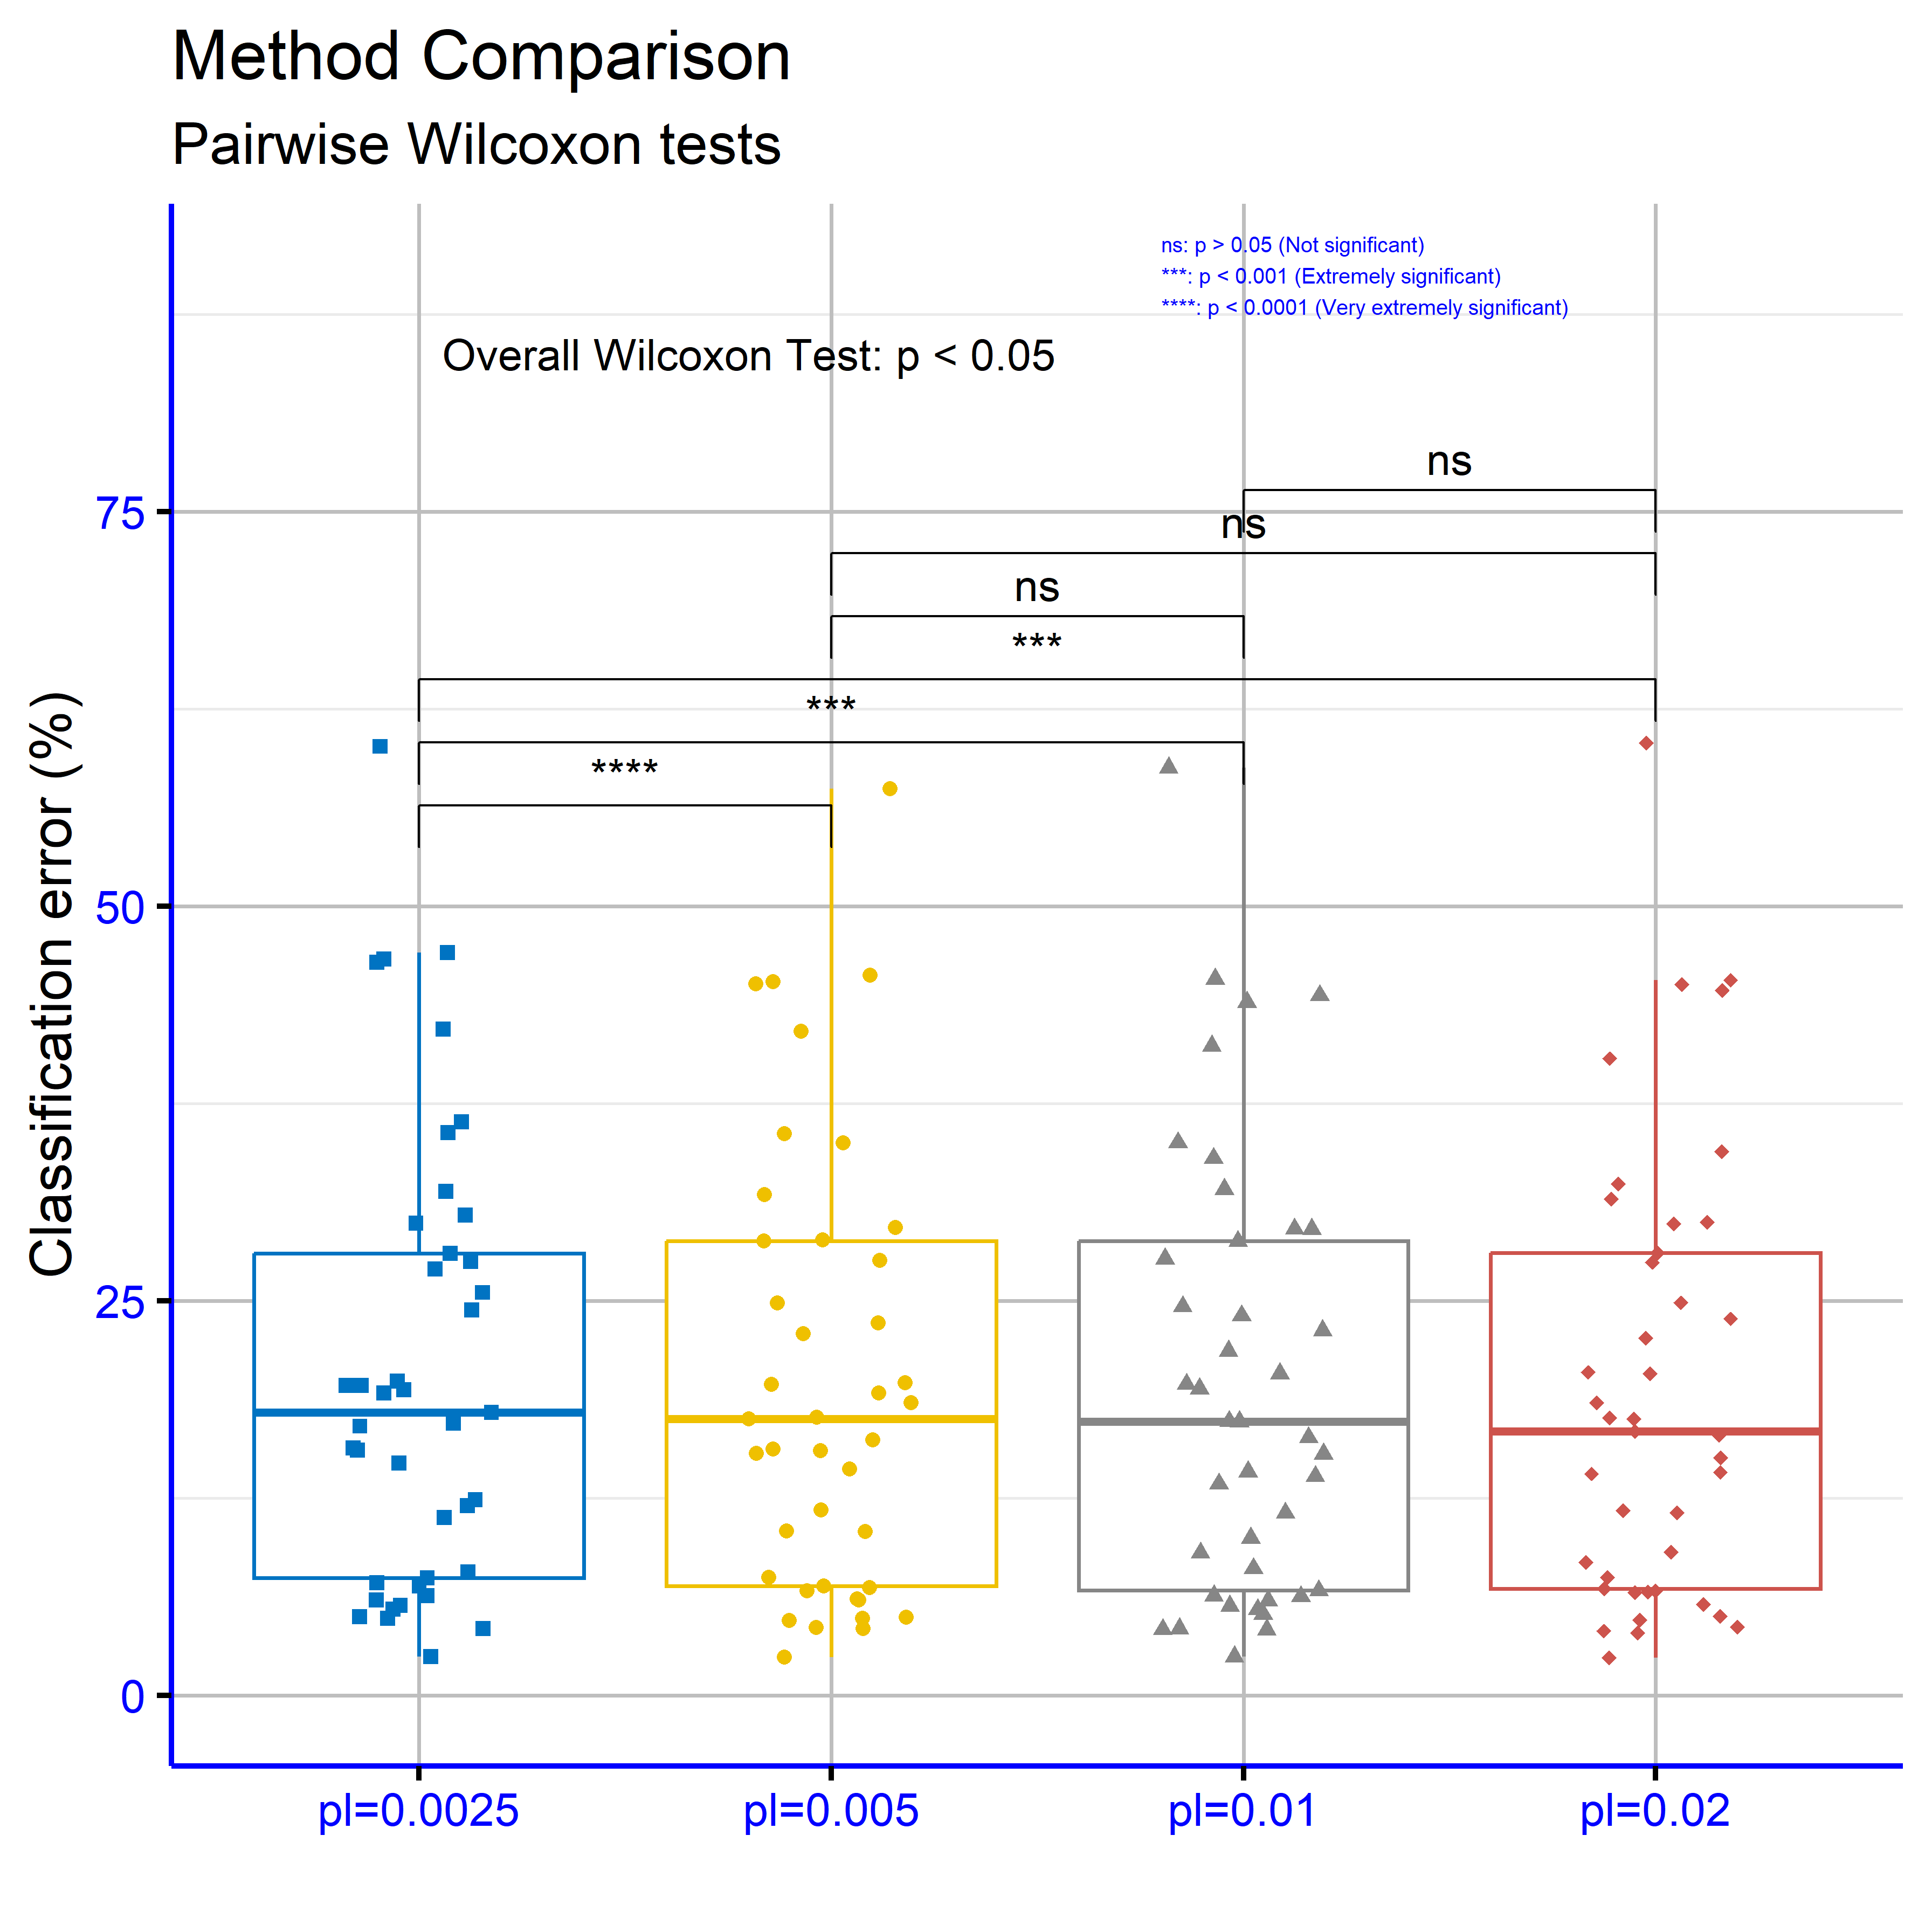
\includegraphics[scale=0.5]{s7}
\par\end{centering}
\caption{Statistical comparison for the conducted experiments on the classification
datasets using the proposed method and different values of local search
rate $p_{l}$.\label{fig:statPLClass}}

\end{figure}

In Figure \ref{fig:statPLRegression}, the regression error for different
values of the periodic local search parameter is presented. In the
comparisons between $p_{l}=0.0025$ and $p_{l}=0.005$, the p-value
was 0.011, indicating a statistically significant difference, as it
is below the significance level of 0.05. In contrast, the comparisons
between $p_{l}=0.0025$ and $p_{l}=0.01$, $p_{l}=0.0025$ and $p_{l}=0.02$,
$p_{l}=0.005$ and $p_{l}=0.01$, and $p_{l}=0.005$ and $p_{l}=0.02$
did not show statistically significant differences, with p-values
of 0.12, 0.18, 0.22, and 0.097, respectively, all of which are above
the significance level of 0.05. Finally, the comparison between $p_{l}=0.01$
and $p_{l}=0.02$ yielded a p-value of 0.086, which is close to but
above the significance level of 0.05, suggesting borderline non-significance.
Overall, the results indicate that only the comparison between $p_{l}=0.0025$
and $p_{l}=0.005$ showed a statistically significant difference,
while the remaining comparisons did not present clear statistically
significant differences.

\begin{figure}[H]
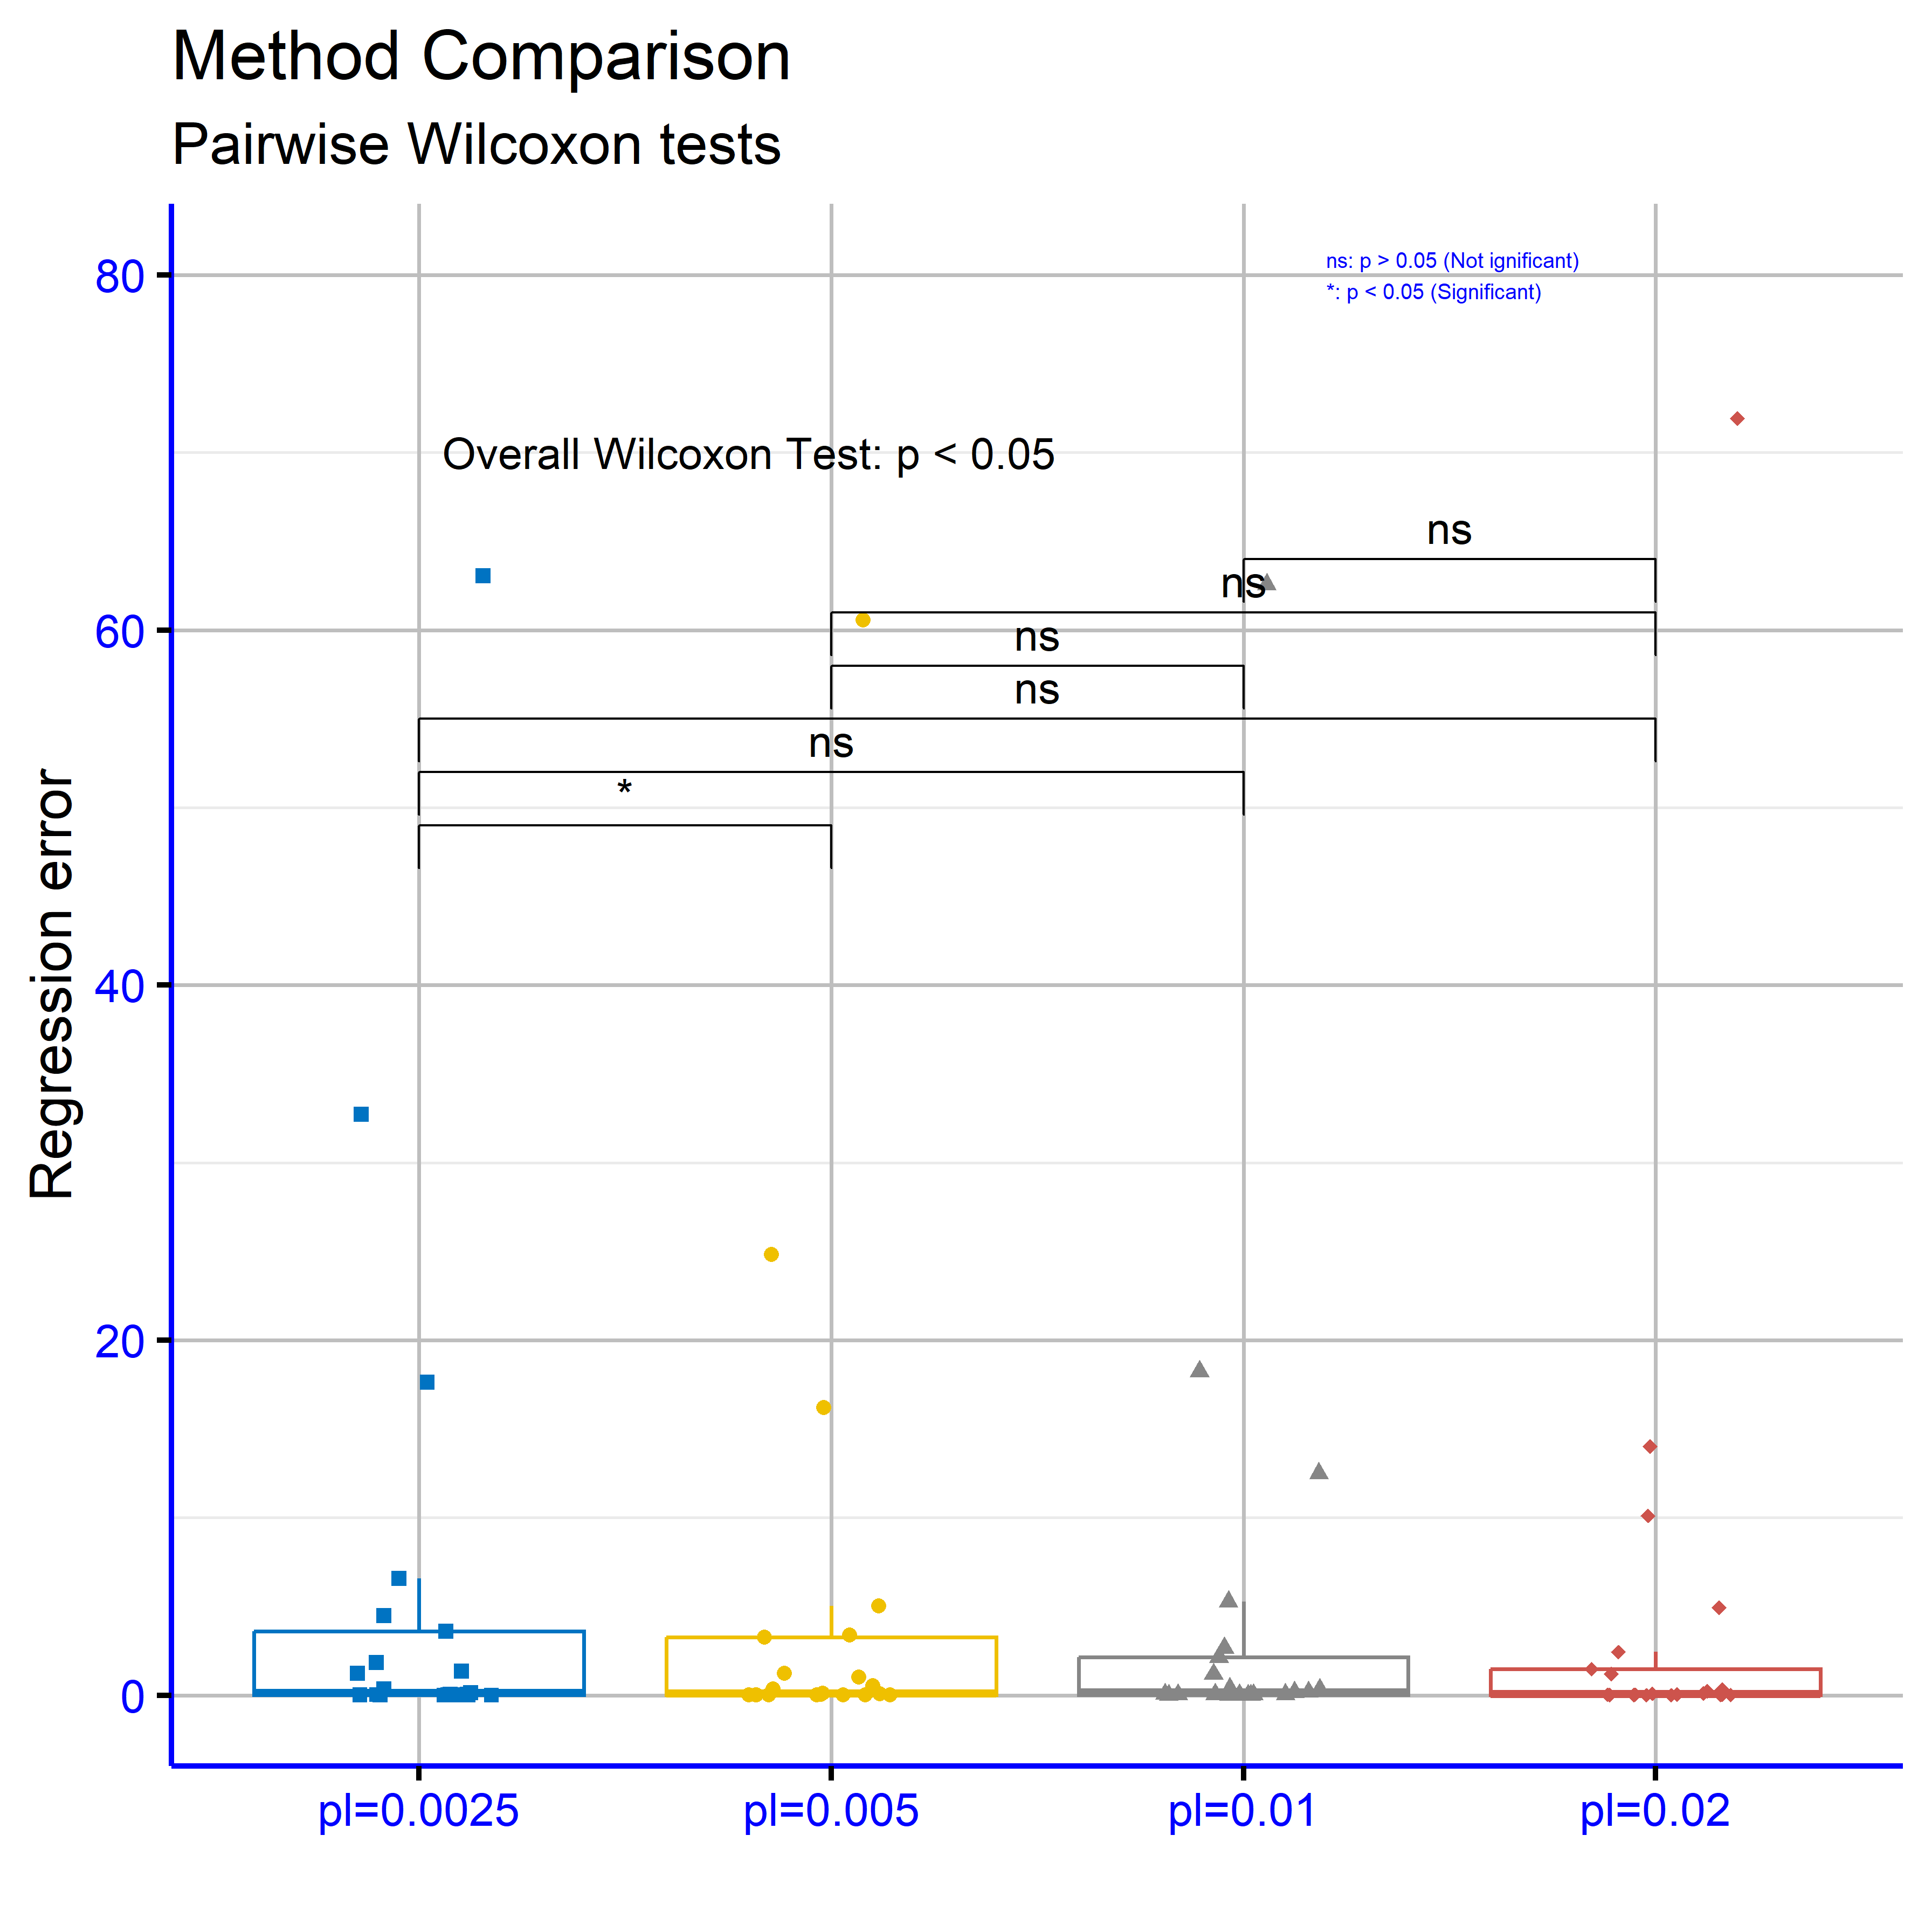
\includegraphics[scale=0.5]{s8}

\caption{Statistical comparison for the conducted experiments on the regression
datasets using the proposed method and different values of local search
rate $p_{l}$.\label{fig:statPLRegression}}

\end{figure}


\subsubsection{Experiments with the local search method}

Another test was conducted, where the local optimization method of
the proposed technique was altered. In this test the local optimization
methods Limited Memory BFGS (LBFGS) \citep{LBFGS} and Adam \citep{Adam}
was used and the results were compared against that obtained by the
application of the BFGS local optimization methods. The experimental
results for the classification datasets are depicted in Table \ref{tab:experLocalClass}
and the experimental results for the regression datasets are shown
in Table \ref{tab:experLocalRegression}.

\begin{table}[H]
\caption{Experimental results for the classification datasets using different
local search methods for the classification datasets. Numbers in cells
stand for the average classification error as measured on the corresponding
test set.\label{tab:experLocalClass}}

\centering{}%
\begin{tabular}{|c|c|c|c|}
\hline 
DATASET & BFGS & LBFGS & ADAM\tabularnewline
\hline 
\hline 
ALCOHOL & 19.15\% & 22.76\% & 19.36\%\tabularnewline
\hline 
AUSTRALIAN & 15.31\% & 21.80\% & 31.19\%\tabularnewline
\hline 
BALANCE & 6.92\% & 7.29\% & 8.08\%\tabularnewline
\hline 
BANDS & 35.00\% & 35.58\% & 35.72\%\tabularnewline
\hline 
CLEVELAND & 45.07\% & 43.76\% & 44.76\%\tabularnewline
\hline 
CIRCULAR & 4.23\% & 4.29\% & 4.52\%\tabularnewline
\hline 
DERMATOLOGY & 10.38\% & 9.09\% & 11.34\%\tabularnewline
\hline 
ECOLI & 45.22\% & 46.43\% & 51.36\%\tabularnewline
\hline 
HABERMAN & 27.55\% & 27.17\% & 27.63\%\tabularnewline
\hline 
HAYES-ROTH & 35.59\% & 37.00\% & 35.38\%\tabularnewline
\hline 
HEART & 17.60\% & 15.93\% & 20.59\%\tabularnewline
\hline 
HEARTATTACK & 19.70\% & 18.57\% & 21.80\%\tabularnewline
\hline 
HEPATITIS & 57.46\% & 56.50\% & 57.25\%\tabularnewline
\hline 
HOUSEVOTES & 7.48\% & 7.74\% & 5.39\%\tabularnewline
\hline 
IONOSPHERE & 16.17\% & 16.57\% & 11.77\%\tabularnewline
\hline 
LIVERDISORDER & 31.72\% & 32.29\% & 33.06\%\tabularnewline
\hline 
LYMOGRAPHY & 28.86\% & 27.93\% & 23.57\%\tabularnewline
\hline 
MAGIC & 11.73\% & 11.83\% & 12.72\%\tabularnewline
\hline 
MAMMOGRAPHIC & 17.52\% & 16.76\% & 17.13\%\tabularnewline
\hline 
PARKINSONS & 14.32\% & 13.58\% & 15.42\%\tabularnewline
\hline 
PAGE BLOCKS & 6.04\% & 5.80\% & 6.78\%\tabularnewline
\hline 
PHONEME & 15.50\% & 15.36\% & 16.93\%\tabularnewline
\hline 
PIMA & 24.85\% & 24.24\% & 30.67\%\tabularnewline
\hline 
POPFAILURES & 6.09\% & 6.74\% & 4.58\%\tabularnewline
\hline 
REGIONS2 & 28.77\% & 29.89\% & 29.58\%\tabularnewline
\hline 
RING & 22.90\% & 23.64\% & 25.66\%\tabularnewline
\hline 
SAHEART & 29.63\% & 28.70\% & 32.18\%\tabularnewline
\hline 
SEGMENT & 15.60\% & 19.46\% & 27.47\%\tabularnewline
\hline 
SONAR & 19.80\% & 19.35\% & 18.65\%\tabularnewline
\hline 
SPAMBASE & 4.95\% & 4.78\% & 3.91\%\tabularnewline
\hline 
SPIRAL & 42.06\% & 41.74\% & 42.84\%\tabularnewline
\hline 
STATHEART & 18.53\% & 17.59\% & 20.22\%\tabularnewline
\hline 
STUDENT & 4.86\% & 5.23\% & 3.82\%\tabularnewline
\hline 
TAE & 45.62\% & 47.20\% & 51.20\%\tabularnewline
\hline 
TRANSFUSION & 23.59\% & 24.32\% & 25.06\%\tabularnewline
\hline 
WDBC & 4.29\% & 4.18\% & 6.00\%\tabularnewline
\hline 
WINE & 10.39\% & 10.06\% & 14.82\%\tabularnewline
\hline 
Z\_F\_S & 6.81\% & 7.10\% & 11.03\%\tabularnewline
\hline 
ZO\_NF\_S & 4.73\% & 5.34\% & 9.72\%\tabularnewline
\hline 
ZONF\_S & 2.41\% & 2.74\% & 3.36\%\tabularnewline
\hline 
ZOO & 6.63\% & 6.20\% & 8.00\%\tabularnewline
\hline 
\textbf{AVERAGE} & \textbf{19.78\%} & \textbf{20.06\%} & \textbf{21.48\%}\tabularnewline
\hline 
\end{tabular}
\end{table}
\begin{table}[H]
\caption{Experimental results for the regression datasets using different local
search methods.\label{tab:experLocalRegression}}

\centering{}%
\begin{tabular}{|c|c|c|c|}
\hline 
DATASET & BFGS & LBFGS & ADAM\tabularnewline
\hline 
\hline 
ABALONE & 5.04 & 4.48 & 4.38\tabularnewline
\hline 
AIRFOIL & 0.0014 & 0.0024 & 0.0031\tabularnewline
\hline 
AUTO & 16.21 & 19.60 & 20.70\tabularnewline
\hline 
BK & 0.019 & 0.017 & 0.018\tabularnewline
\hline 
BL & 0.016 & 0.010 & 0.024\tabularnewline
\hline 
BASEBALL & 60.56 & 49.78 & 78.73\tabularnewline
\hline 
CONCRETE & 0.003 & 0.003 & 0.003\tabularnewline
\hline 
DEE & 0.35 & 0.30 & 0.36\tabularnewline
\hline 
FA & 0.083 & 0.020 & 0.022\tabularnewline
\hline 
FRIEDMAN & 1.22 & 1.23 & 2.29\tabularnewline
\hline 
HO & 0.017 & 0.009 & 0.02\tabularnewline
\hline 
HOUSING & 24.82 & 35.57 & 47.63\tabularnewline
\hline 
LASER & 0.0026 & 0.0027 & 0.0025\tabularnewline
\hline 
LW & 0.021 & 0.012 & 0.015\tabularnewline
\hline 
MORTGAGE & 0.54 & 1.54 & 2.01\tabularnewline
\hline 
PLASTIC & 3.27 & 2.53 & 3.40\tabularnewline
\hline 
PY & 0.11 & 0.09 & 0.04\tabularnewline
\hline 
QUAKE & 0.042 & 0.044 & 0.047\tabularnewline
\hline 
SN & 0.027 & 0.032 & 0.024\tabularnewline
\hline 
STOCK & 3.40 & 8.90 & 11.27\tabularnewline
\hline 
TREASURY & 1.021 & 2.43 & 2.60\tabularnewline
\hline 
\textbf{AVERAGE} & \textbf{5.56} & \textbf{6.03} & \textbf{8.27}\tabularnewline
\hline 
\end{tabular}
\end{table}
The analysis of the Table \ref{tab:experLocalClass} regarding the
local search methods BFGS, LBFGS, and ADAM for the NEURALDE model
presents their performance on classification datasets, with the values
representing error percentages. According to the results, the BFGS
method achieves the lowest average error rate at 19.78\%, followed
by LBFGS with 20.06\% and ADAM with 21.48\%. This highlights the relative
superiority of BFGS in minimizing error compared to the other methods.
When analyzing individual datasets, BFGS records the lowest error
rates in several cases. For instance, in the HOUSEVOTES dataset, both
BFGS and LBFGS yield similar results, while ADAM shows the lowest
error at 5.39\%. In the SPAMBASE dataset, ADAM outperforms the others
with an error rate of 3.91\%, compared to 4.95\% and 4.78\% for BFGS
and LBFGS, respectively. Similarly, in the STUDENT dataset, ADAM performs
best with the lowest error at 3.82\%. However, in datasets like SEGMENT,
BFGS excels with a significantly lower error of 15.60\% compared to
19.46\% for LBFGS and 27.47\% for ADAM. Notable differences are observed
in datasets such as DERMATOLOGY, where LBFGS records the lowest error
at 9.09\%, compared to 10.38\% for BFGS and 11.34\% for ADAM. In the
MAGIC dataset, BFGS and LBFGS deliver comparable performance, with
error rates of 11.73\% and 11.83\%, respectively, while ADAM presents
a higher error of 12.72\%. Similarly, in the CIRCULAR dataset, BFGS
achieves the lowest error at 4.23\%, closely followed by LBFGS at
4.29\%, and ADAM at 4.52\%. Overall, BFGS demonstrates superior performance
in most cases, maintaining the lowest variation in error rates and
achieving the smallest average error. However, LBFGS delivers competitive
results with slightly higher average error and outperforms in specific
datasets like DERMATOLOGY. While ADAM records lower error rates in
isolated datasets such as SPAMBASE and STUDENT, it exhibits a higher
overall error, indicating greater variability in its performance.
In conclusion, the BFGS method emerges as the most efficient overall,
while LBFGS offers consistently competitive performance. ADAM shows
advantages in certain datasets but has a higher overall average error
rate.

The evaluation presented in Table \ref{tab:experLocalRegression}
highlights the performance of the local search methods BFGS, LBFGS,
and ADAM applied to regression datasets within the NEURALDE model.
The reported values correspond to absolute errors. Among the three
methods, BFGS achieves the lowest mean error of 5.56, demonstrating
a clear advantage over LBFGS and ADAM, which have mean errors of 6.03
and 8.27, respectively. Examining individual datasets, BFGS achieves
superior results in several instances. For example, in the AIRFOIL
dataset, it records the smallest error at 0.0014, while LBFGS and
ADAM show slightly higher errors of 0.0024 and 0.0031, respectively.
On the other hand, LBFGS outperforms in the BASEBALL dataset, achieving
the lowest error at 49.78, compared to 60.56 for BFGS and 78.73 for
ADAM. Similarly, LBFGS demonstrates the best performance in the BL
dataset with an error of 0.01, outperforming BFGS and ADAM, which
exhibit errors of 0.016 and 0.024, respectively. In the PLASTIC dataset,
LBFGS again achieves the smallest error at 2.53, followed by BFGS
with 3.27 and ADAM with 3.4. Conversely, in the MORTGAGE dataset,
BFGS performs best, with an error of 0.54, while LBFGS and ADAM display
larger errors of 1.54 and 2.01. In the STOCK dataset, BFGS also demonstrates
superior performance, recording the lowest error at 3.4, whereas LBFGS
and ADAM show significantly higher errors of 8.9 and 11.27, respectively.
Certain datasets exhibit negligible differences in performance among
the methods. For instance, in the CONCRETE dataset, all three methods
produce identical errors of 0.003. Similarly, in the LASER dataset,
the errors are nearly identical, with ADAM achieving 0.0025, BFGS
0.0026, and LBFGS 0.0027. Overall, BFGS emerges as the most effective
method, delivering the lowest average error and consistently strong
results across numerous datasets. LBFGS, while slightly less efficient
on average, demonstrates competitive performance in specific datasets
such as BASEBALL, BL, and PLASTIC. ADAM, though occasionally effective,
as observed in datasets like LASER, shows greater variability and
a higher mean error, limiting its overall reliability. In conclusion,
BFGS stands out as the most robust and dependable method, with LBFGS
showing significant potential in select contexts.

In Figure \ref{fig:statLocalClass}, the critical parameter p, which
indicates the level of statistical significance, showed no statistically
significant difference between the BFGS and LBFGS methods, with p=0.78.
This high value does not meet the common significance threshold (p\textless 0.05).
In contrast, the comparison between BFGS and ADAM revealed a statistically
significant difference, with p=0.0017, indicating clear differentiation
between the two methods. Similarly, the comparison between LBFGS and
ADAM recorded p=0.0031, also below the significance level, proving
that the two methods exhibit statistically significant differences
in classification error performance. 

\begin{figure}[H]
\begin{centering}
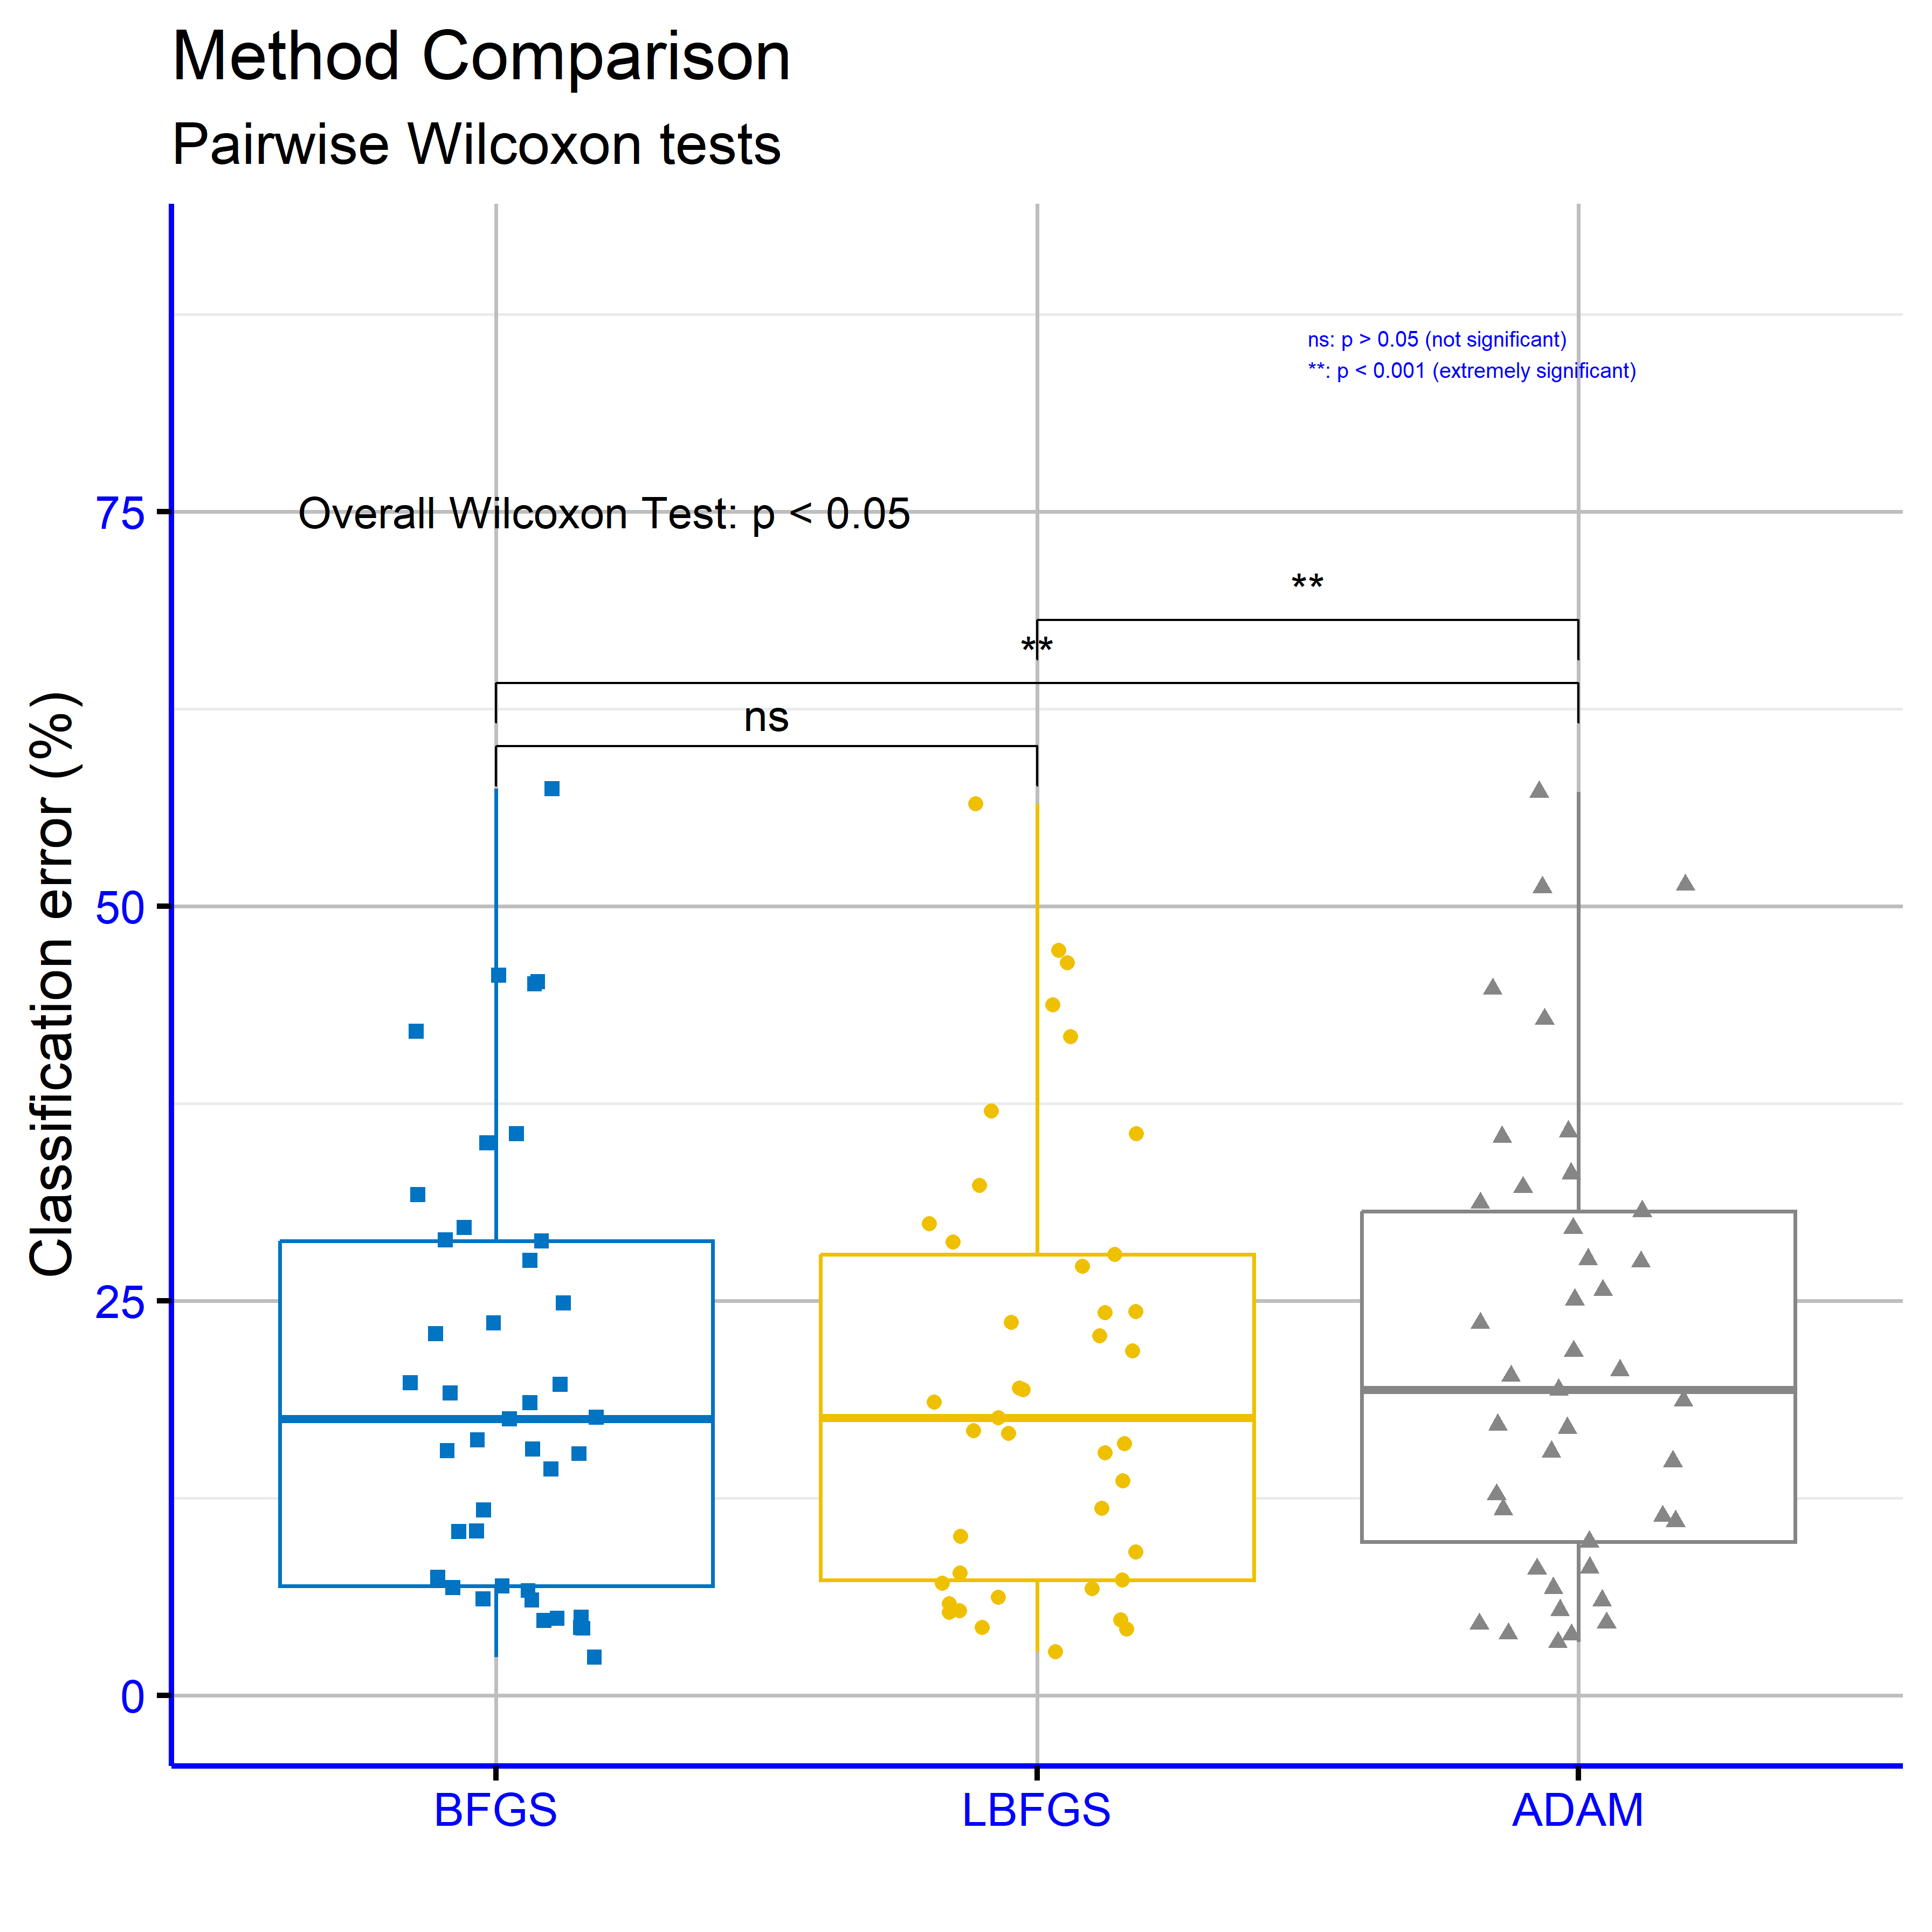
\includegraphics[scale=0.5]{ls1}
\par\end{centering}
\caption{Statistical comparison of the experimental results using the proposed
methods and a variety of local optimization techniques for the classification
datasets.\label{fig:statLocalClass}}

\end{figure}

In Figure \ref{fig:statLocalRegression}, the results showed that
the BFGS and LBFGS methods have no statistically significant difference,
with p=1.0, suggesting that the two methods perform essentially the
same regarding regression error. However, the comparison between BFGS
and ADAM resulted in p=0.037, which is below the 0.05 threshold, highlighting
a statistically significant difference favoring BFGS. Lastly, the
comparison between LBFGS and ADAM recorded p=0.0054, confirming a
statistically significant differentiation between these two methods
as well. In summary, the results of the Wilcoxon Test demonstrate
that BFGS and LBFGS have comparable performances in regression error,
while they do not exhibit statistically significant differences in
classification error. On the other hand, the differences between ADAM
and the other two methods (BFGS and LBFGS) are statistically significant
in both cases, indicating that ADAM shows distinct performance characteristics
in both classification and regression error.

\begin{figure}[H]
\begin{centering}
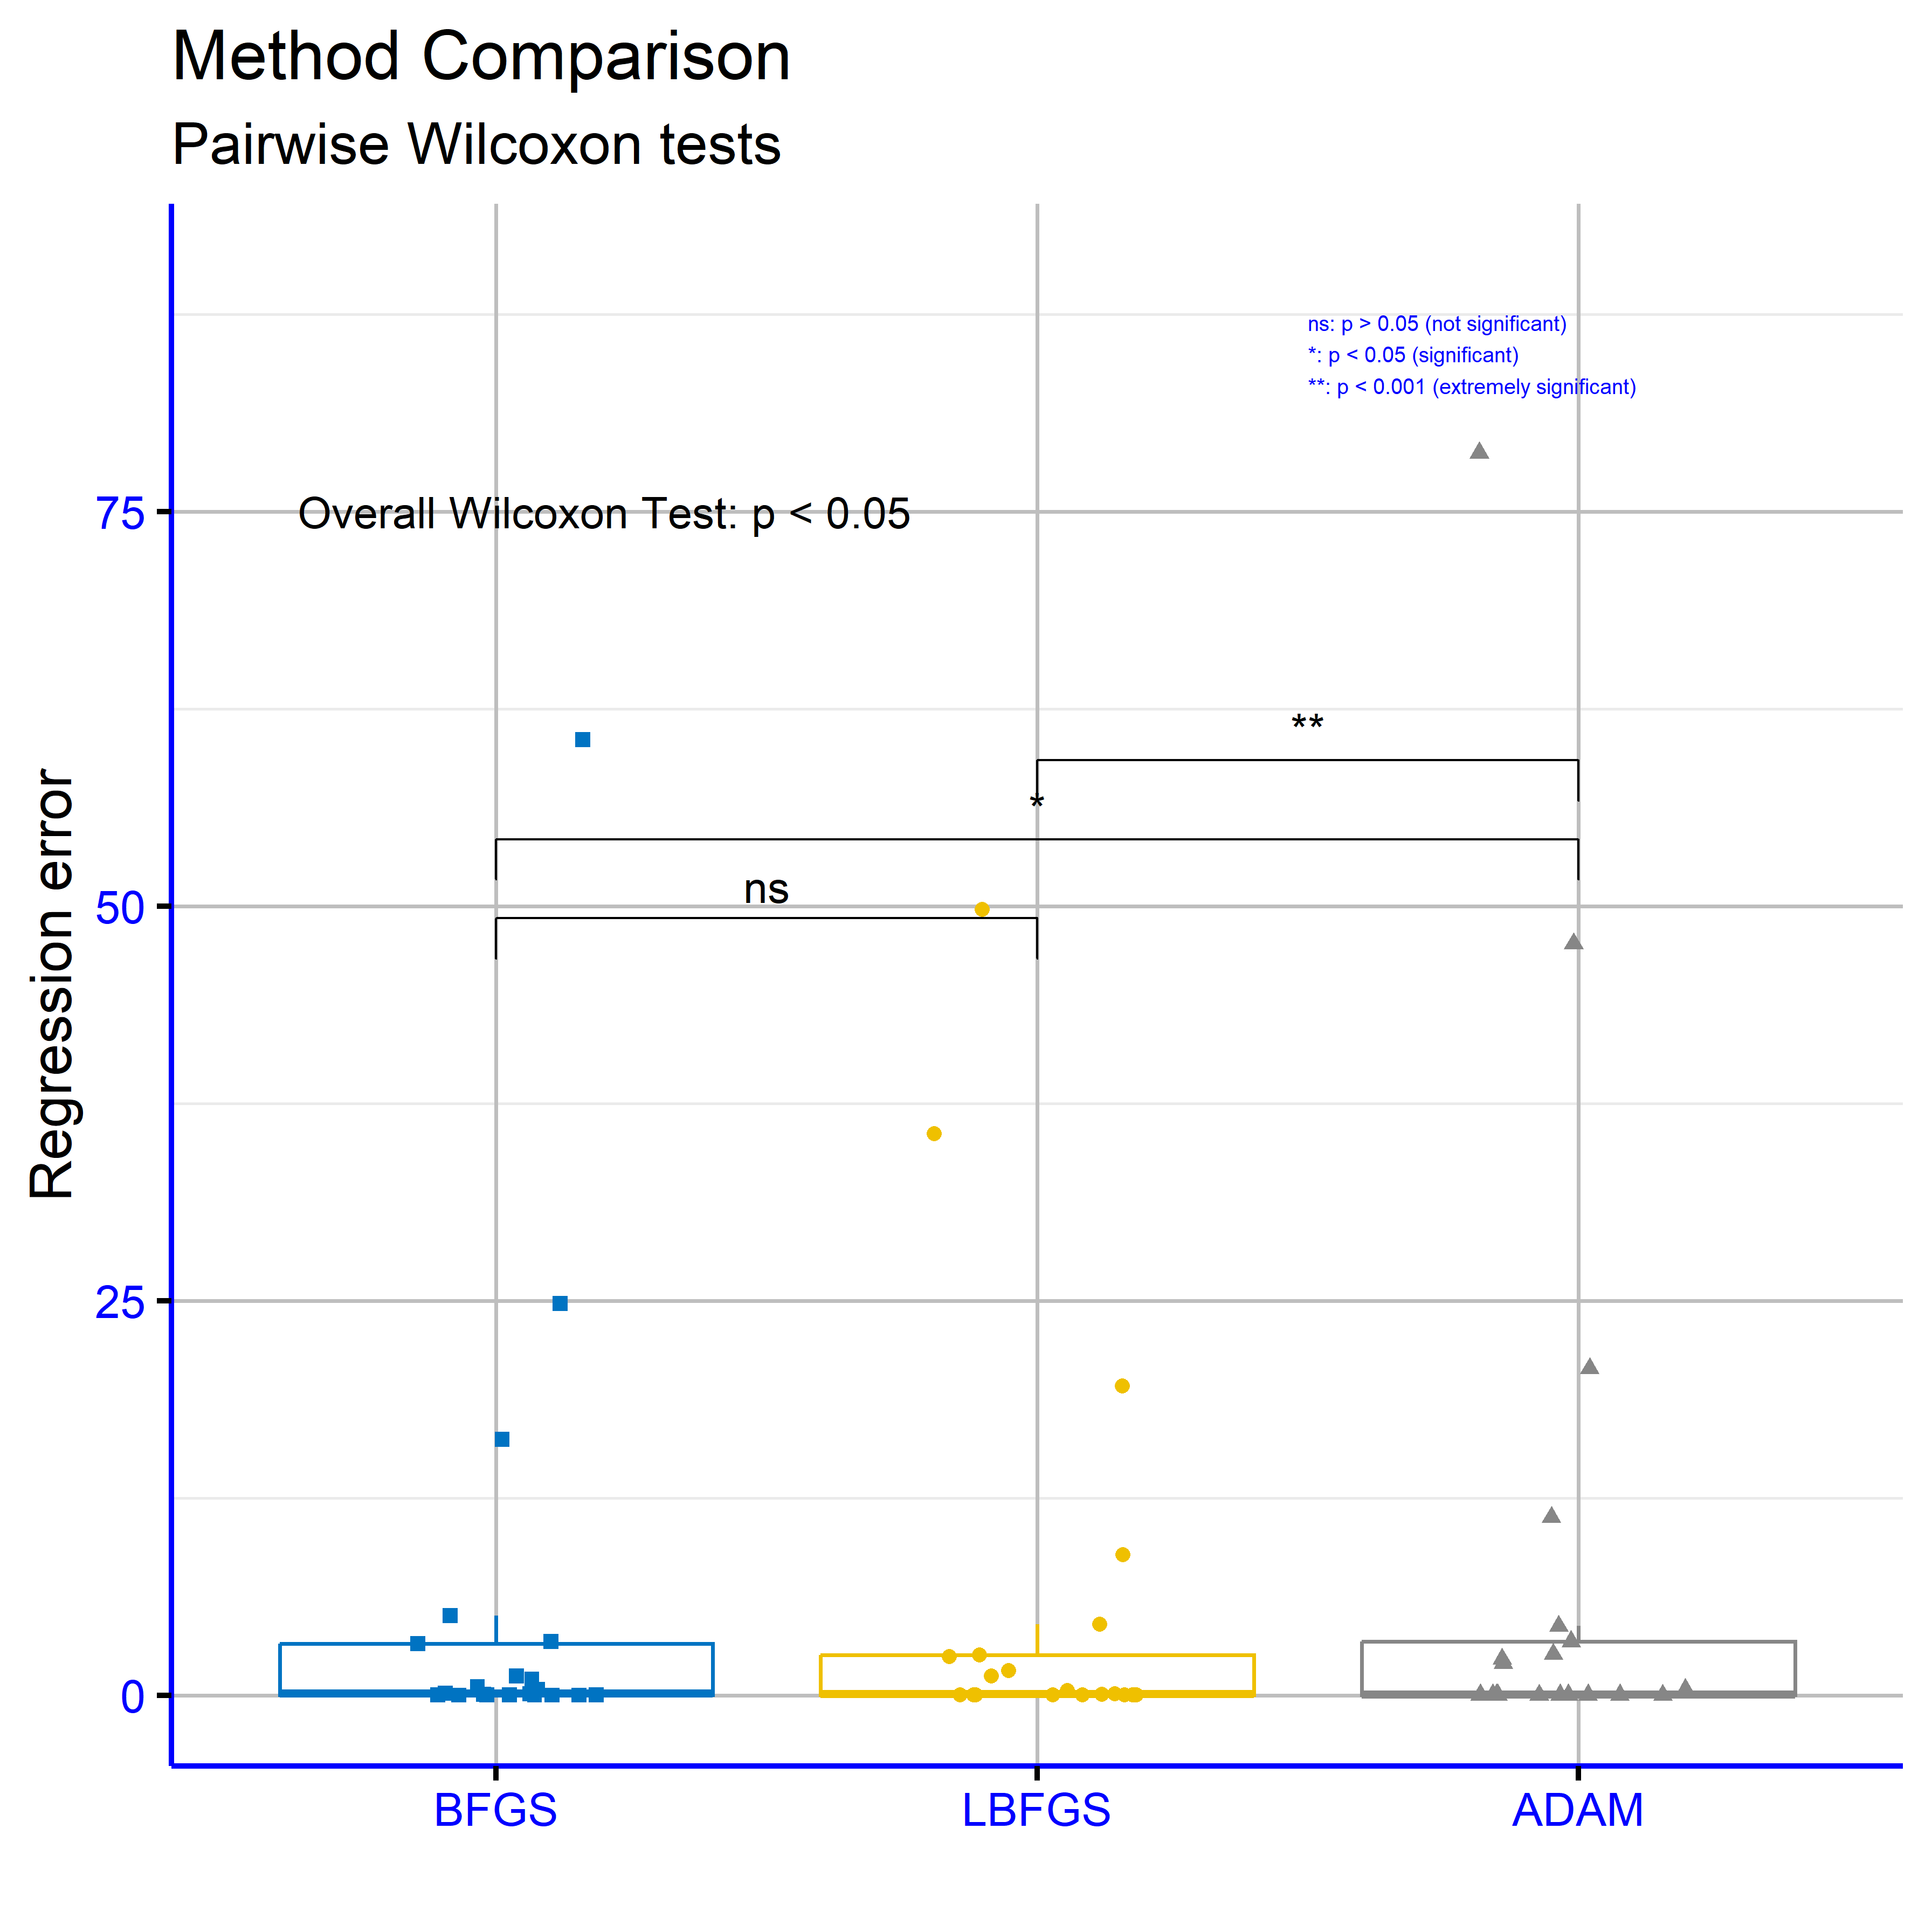
\includegraphics[scale=0.5]{ls2}
\par\end{centering}
\caption{Statistical comparison of the experimental results using a variety
of local optimization methods applied on the regression datasets.\label{fig:statLocalRegression}}

\end{figure}


\subsection{Summary of experimental results}

In conclusion, the analysis conducted on the tables and figures of
the study reveals significant findings regarding the performance of
different machine learning models and parameters. Below is a summary
of the key points of the statistical analysis. The analysis primarily
focuses on the NEURALDE model and its performance compared to other
optimization models (ADAM, BFGS, GENETIC, NEAT, RBF). Non-parametric
statistical tests, such as the Wilcoxon Test, were utilized, which
are suitable for data that do not follow a normal distribution. The
statistically significant differences observed ($p<0.05$) highlight
the consistent superiority of NEURALDE in most cases. Specifically,
the model achieved the lowest average error rate in both classifications
(19.78\%) and regression problems (average error of 5.56), consistently
outperforming its competitors. Similarly, in the tables comparing
different weight computation methods (MIGRANT, ADAPTIVE, RANDOM),
MIGRANT demonstrated the best performance in classifications with
an average error of 19.34\%, while RANDOM excelled in regressions
with an average error of 5.56. The deviations among these methods
warrant further investigation regarding error variability across datasets.
In parameter analysis, the $a$ value (range of optimal values) and
$p_{l}$ (periodic local optimization parameter) appear to influence
performance differently depending on the context. For example, the
$a$ parameter with a value of 2 achieved the lowest average error
in classifications, while for regressions, a value of 1.5 was most
effective. Similarly, for $p_{l}$ the value of 0.02 consistently
showed better performance in classifications, whereas 0.01 proved
more effective for regressions. In summary, the results underline
the importance of selecting the appropriate model and parameters based
on the characteristics of the data. NEURALDE stands out as the most
robust and efficient model, significantly outperforming its competitors.
The specific parameters and methods affect overall performance and
should be carefully evaluated to optimize the system.

\section{Conclusions\label{sec:Conclusions} }

The study focuses on the development and evaluation of the NEURALDE
method, an innovative approach to optimizing neural network training
based on Differential Evolution (DE). The results demonstrate that
NEURALDE outperforms traditional optimization techniques such as ADAM,
BFGS, GENETIC, NEAT, and RBF in both classification and regression
tasks. Across a wide range of datasets, NEURALDE consistently achieved
the lowest error rates, confirming its robustness and efficiency.
Statistical analyses, including the Wilcoxon Test, were used to validate
the significance of the differences between NEURALDE and other methods.
The extremely low p-values indicate that the observed differences
are not random but reflect the actual superiority of NEURALDE. Furthermore,
the method proved resilient to common neural network training challenges,
such as overfitting and entrapment in local minima. 

NEURALDE is established as a reliable and high-performance optimization
method for machine learning applications. Its exceptional performance
in both classification and regression, combined with statistical validation
of its superiority, positions it as a strong contender for broader
adoption in various machine learning applications. The method is particularly
useful for complex datasets or scenarios where traditional approaches
fail to deliver satisfactory results. 

This study opens multiple avenues for further research. Firstly, exploring
the scalability of NEURALDE on larger and more diverse datasets could
provide valuable insights into its generalizability and practical
utility. Incorporating adaptive mechanisms within the Differential
Evolution framework is another promising direction, as it could dynamically
adjust parameters based on dataset characteristics, further enhancing
the method’s performance. Another interesting avenue is applying NEURALDE
to unsupervised learning tasks, such as clustering, to evaluate its
adaptability across different machine learning paradigms. Furthermore,
integrating NEURALDE with cutting-edge techniques like transfer learning
and reinforcement learning could unlock new potential, particularly
for real-time applications and complex decision-making environments.
Future research could also focus on reducing the computational cost
of the method to make it more accessible for large-scale problems.
Overall, NEURALDE provides a robust foundation for further improvements
and extensions, aiming to establish it as a key optimization method
in machine learning.

However, the proposed technique exhibits significantly increased execution
time compared to the original training algorithm due to the periodic
use of the differential evolution technique.\textbf{ }These problems
can be circumvented by using parallel processing techniques such as
the MPI interface \citep{openmpi} and the OpenMP programming library
\citep{openmp}. Also, parallel approaches of the Differential Evolution
\citep{pde1,pde2} ttechnique could also be incorporated to significantly
reduce the required computing time.

\vspace{6pt}


\authorcontributions{I.G.T. conceptualized the idea and methodology, supervised the technical
aspects related to the software, and contributed to manuscript preparation.
Also, I.G.T conducted the experiments using various datasets and V.C.
performed statistical analysis. I.G.T and V.C prepared the manuscript
for publication. All authors have reviewed and endorsed the conclusive
version of the manuscript.}

\funding{This research received no external funding.}

\institutionalreview{Not applicable.}

\informedconsent{Not applicable. }

\institutionalreview{Not applicable.}

\acknowledgments{This research has been financed by the European Union : Next Generation
EU through the Program Greece 2.0 National Recovery and Resilience
Plan , under the call RESEARCH -- CREATE -- INNOVATE, project name
“iCREW: Intelligent small craft simulator for advanced crew training
using Virtual Reality techniques\textquotedbl{} (project code:TAEDK-06195).}

\conflictsofinterest{The authors declare no conflict of interest.}

\appendixtitles{}

\appendixstart{}

\appendix

\begin{adjustwidth}{-\extralength}{0cm}{}

\reftitle{References}
\begin{thebibliography}{99}
\bibitem{nn1}C. Bishop, Neural Networks for Pattern Recognition,
Oxford University Press, 1995.

\bibitem{nn2}G. Cybenko, Approximation by superpositions of a sigmoidal
function, Mathematics of Control Signals and Systems \textbf{2}, pp.
303-314, 1989.

\bibitem{nnphysics1}P. Baldi, K. Cranmer, T. Faucett et al, Parameterized
neural networks for high-energy physics, Eur. Phys. J. C \textbf{76},
2016.

\bibitem{nnphysics2}Baldi, P., Cranmer, K., Faucett, T., Sadowski,
P., \& Whiteson, D. (2016). Parameterized neural networks for high-energy
physics. The European Physical Journal C, 76(5), 1-7.

\bibitem{nnphysics3}G. Carleo,M. Troyer, Solving the quantum many-body
problem with artificial neural networks, Science \textbf{355}, pp.
602-606, 2017.

\bibitem{nnde1}Khoo, Y., Lu, J., \& Ying, L. (2021). Solving parametric
PDE problems with artificial neural networks. European Journal of
Applied Mathematics, 32(3), 421-435.

\bibitem{nn_solar}A. Kumar Yadav, S.S. Chandel, Solar radiation prediction
using Artificial Neural Network techniques: A review, Renewable and
Sustainable Energy Reviews \textbf{33}, pp. 772-781, 2014.

\bibitem{nnagr2}A. Escamilla-García, G.M. Soto-Zarazúa, M. Toledano-Ayala,
E. Rivas-Araiza, A. Gastélum-Barrios, Abraham,Applications of Artificial
Neural Networks in Greenhouse Technology and Overview for Smart Agriculture
Development, Applied Sciences \textbf{10}, Article number 3835, 2020.

\bibitem{nnchem1}Lin Shen, Jingheng Wu, and Weitao Yang, Multiscale
Quantum Mechanics/Molecular Mechanics Simulations with Neural Networks,
Journal of Chemical Theory and Computation \textbf{12}, pp. 4934-4946,
2016.

\bibitem{nnchem3}Jennifer N. Wei, David Duvenaud, and Alán Aspuru-Guzik,
Neural Networks for the Prediction of Organic Chemistry Reactions,
ACS Central Science \textbf{2}, pp. 725-732, 2016.

\bibitem{nnecon1}Lukas Falat and Lucia Pancikova, Quantitative Modelling
in Economics with Advanced Artificial Neural Networks, Procedia Economics
and Finance \textbf{34}, pp. 194-201, 2015.

\bibitem{nnecon2}Mohammad Namazi, Ahmad Shokrolahi, Mohammad Sadeghzadeh
Maharluie, Detecting and ranking cash flow risk factors via artificial
neural networks technique, Journal of Business Research \textbf{69},
pp. 1801-1806, 2016.

\bibitem{nnmed1}Igor I. Baskin, David Winkler and Igor V. Tetko,
A renaissance of neural networks in drug discovery, Expert Opinion
on Drug Discovery \textbf{11}, pp. 785-795, 2016.

\bibitem{nnmed2}Ronadl Bartzatt, Prediction of Novel Anti-Ebola Virus
Compounds Utilizing Artificial Neural Network (ANN), Chemistry Faculty
Publications \textbf{49}, pp. 16-34, 2018.

\bibitem{bpnn1}D.E. Rumelhart, G.E. Hinton and R.J. Williams, Learning
representations by back-propagating errors, Nature \textbf{323}, pp.
533 - 536 , 1986.

\bibitem{bpnn2}Shihab, K. (2006). A backpropagation neural network
for computer network security. Journal of Computer Science, 2(9),
710-715.

\bibitem{rpropnn-1}M. Riedmiller and H. Braun, A Direct Adaptive
Method for Faster Backpropagation Learning: The RPROP algorithm, Proc.
of the IEEE Intl. Conf. on Neural Networks, San Francisco, CA, pp.
586--591, 1993.

\bibitem{Adam}D. P. Kingma, J. L. Ba, ADAM: a method for stochastic
optimization, in: Proceedings of the 3rd International Conference
on Learning Representations (ICLR 2015), pp. 1--15, 2015.

\bibitem{nn_ann1}A. Yamazaki, M. C. P. de Souto,T. B. Ludermir, Optimization
of neural network weights and architectures for odor recognition using
simulated annealing, In: Proceedings of the 2002 International Joint
Conference on Neural Networks. IJCNN'02 \textbf{1}, pp. 547-552 ,
2002.

\bibitem{geneticnn}F. H. F. Leung, H. K. Lam, S. H. Ling and P. K.
S. Tam, Tuning of the structure and parameters of a neural network
using an improved genetic algorithm, IEEE Transactions on Neural Networks
\textbf{14}, pp. 79-88, 2003

\bibitem{psonn}C. Zhang, H. Shao and Y. Li, Particle swarm optimization
for evolving artificial neural network, IEEE International Conference
on Systems, Man, and Cybernetics, , pp. 2487-2490, 2000.

\bibitem{weight_aco}K.M. Salama, A.M. Abdelbar, Learning neural network
structures with ant colony algorithms, Swarm Intell \textbf{9}, pp.
229--265, 2015.

\bibitem{tabunn}R.S. Sexton, B. Alidaee, R.E. Dorsey, J.D. Johnson,
Global optimization for artificial neural networks: A tabu search
application. European Journal of Operational Research \textbf{106},
pp. 570-584, 1998.

\bibitem{nn_hybrid}J.-R. Zhang, J. Zhang, T.-M. Lok, M.R. Lyu, A
hybrid particle swarm optimization--back-propagation algorithm for
feedforward neural network training, Applied Mathematics and Computation
\textbf{185}, pp. 1026-1037, 2007.

\bibitem{nn_cascade}G. Zhao, T. Wang, Y. Jin, C. Lang, Y. Li, H.
Ling, The Cascaded Forward algorithm for neural network training,
Pattern Recognition \textbf{161}, 111292, 2025.

\bibitem{weight_abc}D. Karaboga and B. Akay, \textquotedbl Artificial
Bee Colony (ABC) Algorithm on Training Artificial Neural Networks,\textquotedbl{}
2007 IEEE 15th Signal Processing and Communications Applications,
Eskisehir, Turkey, 2007, pp. 1-4, doi: 10.1109/SIU.2007.4298679.

\bibitem{nn_init1}T.M. Varnava, A.J.Meade, An initialization method
for feedforward artificial neural networks using polynomial bases,
Advances in Adaptive Data Analysis \textbf{3}, pp. 385-400, 2011.

\bibitem{nn_init2}I. Ivanova, M. Kubat, Initialization of neural
networks by means of decision trees, Knowledge-Based Systems \textbf{8},
pp. 333-344, 1995.

\bibitem{nn_init3}S.S. Sodhi, P. Chandra, Interval based Weight Initialization
Method for Sigmoidal Feedforward Artificial Neural Networks, AASRI
Procedia \textbf{6}, pp. 19-25, 2014.

\bibitem{nn_init4}K. Chumachenko, A. Iosifidis, M. Gabbouj, Feedforward
neural networks initialization based on discriminant learning, Neural
Networks \textbf{146}, pp. 220-229, 2022.

\bibitem{nn_arch1}J. Arifovic, R. Gençay, Using genetic algorithms
to select architecture of a feedforward artificial neural network,
Physica A: Statistical Mechanics and its Applications \textbf{289},
pp. 574-594, 2001.

\bibitem{nn_arch2}P.G. Benardos, G.C. Vosniakos, Optimizing feedforward
artificial neural network architecture, Engineering Applications of
Artificial Intelligence \textbf{20}, pp. 365-382, 2007.

\bibitem{nn_arch3}B.A. Garro, R.A. Vázquez, Designing Artificial
Neural Networks Using Particle Swarm Optimization Algorithms, Computational
Intelligence and Neuroscience, 369298, 2015. 

\bibitem{nn_arch4}B. Baker, O. Gupta, N. Naik, R. Raskar, Designing
neural network architectures using reinforcement learning. arXiv preprint
arXiv:1611.02167, 2016.

\bibitem{nnsharing1}S.J. Nowlan and G.E. Hinton, Simplifying neural
networks by soft weight sharing, Neural Computation 4, pp. 473-493,
1992.

\bibitem{nnsharing2}Nowlan, S. J., \& Hinton, G. E. (2018). Simplifying
neural networks by soft weight sharing. In The mathematics of generalization
(pp. 373-394). CRC Press.

\bibitem{nnprunning1}S.J. Hanson and L.Y. Pratt, Comparing biases
for minimal network construction with back propagation, In D.S. Touretzky
(Ed.), Advances in Neural Information Processing Systems, Volume 1,
pp. 177-185, San Mateo, CA: Morgan Kaufmann, 1989.

\bibitem{nnprunning2}M. Augasta and T. Kathirvalavakumar, Pruning
algorithms of neural networks --- a comparative study, Central European
Journal of Computer Science, 2003.

\bibitem{nnearly1}Lutz Prechelt, Automatic early stopping using cross
validation: quantifying the criteria, Neural Networks \textbf{11},
pp. 761-767, 1998.

\bibitem{nnearly2}X. Wu and J. Liu, A New Early Stopping Algorithm
for Improving Neural Network Generalization, 2009 Second International
Conference on Intelligent Computation Technology and Automation, Changsha,
Hunan, 2009, pp. 15-18.

\bibitem{nndecay1}N. K. Treadgold and T. D. Gedeon, Simulated annealing
and weight decay in adaptive learning: the SARPROP algorithm,IEEE
Transactions on Neural Networks \textbf{9}, pp. 662-668, 1998.

\bibitem{nndecay2}M. Carvalho and T. B. Ludermir, Particle Swarm
Optimization of Feed-Forward Neural Networks with Weight Decay, 2006
Sixth International Conference on Hybrid Intelligent Systems (HIS'06),
Rio de Janeiro, Brazil, 2006, pp. 5-5.

\bibitem{de_review}Pant, M., Zaheer, H., Garcia-Hernandez, L., \&
Abraham, A. (2020). Differential Evolution: A review of more than
two decades of research. Engineering Applications of Artificial Intelligence,
90, 103479.

\bibitem{de1}Storn, R., \& Price, K. (1995). Differential evolution-a
simple and efficient adaptive scheme for global optimization over
continuous spaces. International computer science institute.

\bibitem{de2}Storn, R., \& Price, K. (1997). Differential evolution--a
simple and efficient heuristic for global optimization over continuous
spaces. Journal of global optimization, 11, 341-359.

\bibitem{de_symmetry1}Y.H. Li, J.Q. Wang, X.J. Wang, Y.L. Zhao, X.H.
Lu, D.L. Liu, Community Detection Based on Differential Evolution
Using Social Spider Optimization, Symmetry \textbf{9}, 2017.

\bibitem{de_symmetry3}W. Yang, E.M. Dilanga Siriwardane, R. Dong,
Y. Li, J. Hu, Crystal structure prediction of materials with high
symmetry using differential evolution, J. Phys.: Condens. Matter \textbf{33}
455902, 2021.

\bibitem{de_symmetry6}C.Y. Lee, C.H. Hung, Feature Ranking and Differential
Evolution for Feature Selection in Brushless DC Motor Fault Diagnosis
, Symmetry \textbf{13}, 2021.

\bibitem{de_symmetry7}S. Saha, R. Das, Exploring differential evolution
and particle swarm optimization to develop some symmetry-based automatic
clustering techniques: application to gene clustering, Neural Comput
\& Applic \textbf{30}, pp. 735--757, 2018.

\bibitem[(1989)]{uci} M. Kelly, R. Longjohn, K. Nottingham, The UCI
Machine Learning Repository, https://archive.ics.uci.edu.

\bibitem{key-16}Maulik, U., \& Saha, I. (2010). Automatic fuzzy clustering
using modified differential evolution for image classification. IEEE
transactions on Geoscience and Remote sensing, 48(9), 3503-3510.

\bibitem{de_problem2}Zhang, Y., Zhang, H., Cai, J., \& Yang, B. (2014).
A weighted voting classifier based on differential evolution. In Abstract
and applied analysis (Vol. 2014, No. 1, p. 376950). Hindawi Publishing
Corporation.

\bibitem{de_problem3}Hancer, E. (2019). Differential evolution for
feature selection: a fuzzy wrapper--filter approach. Soft Computing,
23, 5233-5248.

\bibitem{de_problem4}Vivekanandan, T., \& Iyengar, N. C. S. N. (2017).
Optimal feature selection using a modified differential evolution
algorithm and its effectiveness for prediction of heart disease. Computers
in biology and medicine, 90, 125-136.

\bibitem{de_deep1}Deng, W., Liu, H., Xu, J., Zhao, H., \& Song, Y.
(2020). An improved quantum-inspired differential evolution algorithm
for deep belief network. IEEE Transactions on Instrumentation and
Measurement, 69(10), 7319-7327.

\bibitem{de_deep2}Wu, T., Li, X., Zhou, D., Li, N., \& Shi, J. (2021).
Differential evolution based layer-wise weight pruning for compressing
deep neural networks. Sensors, 21(3), 880.

\bibitem{nn_deep1}Sze, V., Chen, Y. H., Yang, T. J., \& Emer, J.
S. (2017). Efficient processing of deep neural networks: A tutorial
and survey. Proceedings of the IEEE, 105(12), 2295-2329.

\bibitem{nn_deep2}Samek, W., Montavon, G., Lapuschkin, S., Anders,
C. J., \& Müller, K. R. (2021). Explaining deep neural networks and
beyond: A review of methods and applications. Proceedings of the IEEE,
109(3), 247-278.

\bibitem{nnc}I.G. Tsoulos, D. Gavrilis, E. Glavas, Neural network
construction and training using grammatical evolution, Neurocomputing
\textbf{72}, pp. 269-277, 2008.

\bibitem{Hornik}Hornik, K., Stinchcombe, M., \& White, H. (1989).
Multilayer feedforward networks are universal approximators. Neural
networks, 2(5), 359-366.

\bibitem[Author1(year)]{de_char} V. Charilogis, I.G. Tsoulos, A.
Tzallas, E. Karvounis, Modifications for the Differential Evolution
Algorithm, Symmetry \textbf{14}, 447, 2022.

\bibitem{powell}M.J.D Powell, A Tolerant Algorithm for Linearly Constrained
Optimization Calculations, Mathematical Programming \textbf{45}, pp.
547-566, 1989. 

\bibitem{Keel}J. Alcalá-Fdez, A. Fernandez, J. Luengo, J. Derrac,
S. García, L. Sánchez, F. Herrera. KEEL Data-Mining Software Tool:
Data Set Repository, Integration of Algorithms and Experimental Analysis
Framework. Journal of Multiple-Valued Logic and Soft Computing 17,
pp. 255-287, 2011.

\bibitem[Tzimourta(2018)]{alcohol}Tzimourta, K.D.; Tsoulos, I.; Bilero,
I.T.; Tzallas, A.T.; Tsipouras, M.G.; Giannakeas, N. Direct Assessment
of Alcohol Consumption in Mental State Using Brain Computer Interfaces
and Grammatical Evolution. Inventions 2018, 3, 51.

\bibitem[Quinlan(2018)]{australian}J.R. Quinlan, Simplifying Decision
Trees. International Journal of Man-Machine Studies \textbf{27}, pp.
221-234, 1987. 

\bibitem[Evans(1994)]{bands}B. Evans, D. Fisher, Overcoming process
delays with decision tree induction. IEEE Expert \textbf{9}, pp. 60-66,
1994.

\bibitem{balance}T. Shultz, D. Mareschal, W. Schmidt, Modeling Cognitive
Development on Balance Scale Phenomena, Machine Learning \textbf{16},
pp. 59-88, 1994.

\bibitem[(2004)]{cleveland1}Z.H. Zhou,Y. Jiang, NeC4.5: neural ensemble
based C4.5,\textquotedbl{} in IEEE Transactions on Knowledge and Data
Engineering \textbf{16}, pp. 770-773, 2004.

\bibitem{cleveland2}R. Setiono , W.K. Leow, FERNN: An Algorithm for
Fast Extraction of Rules from Neural Networks, Applied Intelligence
\textbf{12}, pp. 15-25, 2000.

\bibitem[(1998)]{dermatology}G. Demiroz, H.A. Govenir, N. Ilter,
Learning Differential Diagnosis of Eryhemato-Squamous Diseases using
Voting Feature Intervals, Artificial Intelligence in Medicine. \textbf{13},
pp. 147--165, 1998.

\bibitem[(1996)]{ecoli}P. Horton, K.Nakai, A Probabilistic Classification
System for Predicting the Cellular Localization Sites of Proteins,
In: Proceedings of International Conference on Intelligent Systems
for Molecular Biology \textbf{4}, pp. 109-15, 1996.

\bibitem[(1977)]{hayes-roth}B. Hayes-Roth, B., F. Hayes-Roth. Concept
learning and the recognition and classification of exemplars. Journal
of Verbal Learning and Verbal Behavior \textbf{16}, pp. 321-338, 1977.

\bibitem[(1997)]{heart}I. Kononenko, E. Šimec, M. Robnik-Šikonja,
Overcoming the Myopia of Inductive Learning Algorithms with RELIEFF,
Applied Intelligence \textbf{7}, pp. 39--55, 1997

\bibitem[(2002)]{housevotes}R.M. French, N. Chater, Using noise to
compute error surfaces in connectionist networks: a novel means of
reducing catastrophic forgetting, Neural Comput. \textbf{14}, pp.
1755-1769, 2002.

\bibitem[(2004)]{ion1}J.G. Dy , C.E. Brodley, Feature Selection for
Unsupervised Learning, The Journal of Machine Learning Research \textbf{5},
pp 845--889, 2004.

\bibitem{ion2}S. J. Perantonis, V. Virvilis, Input Feature Extraction
for Multilayered Perceptrons Using Supervised Principal Component
Analysis, Neural Processing Letters \textbf{10}, pp 243--252, 1999.

\bibitem[(2002)]{liver} J. Garcke, M. Griebel, Classification with
sparse grids using simplicial basis functions, Intell. Data Anal.
\textbf{6}, pp. 483-502, 2002.

\bibitem{liver1}J. Mcdermott, R.S. Forsyth, Diagnosing a disorder
in a classification benchmark, Pattern Recognition Letters \textbf{73},
pp. 41-43, 2016.

\bibitem[(2002)]{lymography}G. Cestnik, I. Konenenko, I. Bratko,
Assistant-86: A Knowledge-Elicitation Tool for Sophisticated Users.
In: Bratko, I. and Lavrac, N., Eds., Progress in Machine Learning,
Sigma Press, Wilmslow, pp. 31-45, 1987. 

\bibitem[(2002)]{magic}Heck, D., Knapp, J., Capdevielle, J. N., Schatz,
G., \& Thouw, T. (1998). CORSIKA: A Monte Carlo code to simulate extensive
air showers.

\bibitem[(2007)]{mammographic}M. Elter, R. Schulz-Wendtland, T. Wittenberg,
The prediction of breast cancer biopsy outcomes using two CAD approaches
that both emphasize an intelligible decision process, Med Phys. \textbf{34},
pp. 4164-72, 2007.

\bibitem[(2007)]{parkinsons1}M.A. Little, P.E. McSharry, S.J Roberts
et al, Exploiting Nonlinear Recurrence and Fractal Scaling Properties
for Voice Disorder Detection. BioMed Eng OnLine \textbf{6}, 23, 2007.

\bibitem{parkinsons2}M.A. Little, P.E. McSharry, E.J. Hunter, J.
Spielman, L.O. Ramig, Suitability of dysphonia measurements for telemonitoring
of Parkinson's disease. IEEE Trans Biomed Eng. \textbf{56}, pp. 1015-1022,
2009.

\bibitem[(2007)]{pima}J.W. Smith, J.E. Everhart, W.C. Dickson, W.C.
Knowler, R.S. Johannes, Using the ADAP learning algorithm to forecast
the onset of diabetes mellitus, In: Proceedings of the Symposium on
Computer Applications and Medical Care IEEE Computer Society Press,
pp.261-265, 1988.

\bibitem{pageblocks}F. Esposito F., D. Malerba, G. Semeraro, Multistrategy
Learning for Document Recognition, Applied Artificial Intelligence
\textbf{8}, pp. 33-84, 1994. 

\bibitem[(2007)]{popfailures}D.D. Lucas, R. Klein, J. Tannahill,
D. Ivanova, S. Brandon, D. Domyancic, Y. Zhang, Failure analysis of
parameter-induced simulation crashes in climate models, Geoscientific
Model Development \textbf{6}, pp. 1157-1171, 2013.

\bibitem[(2007)]{regions2}N. Giannakeas, M.G. Tsipouras, A.T. Tzallas,
K. Kyriakidi, Z.E. Tsianou, P. Manousou, A. Hall, E.C. Karvounis,
V. Tsianos, E. Tsianos, A clustering based method for collagen proportional
area extraction in liver biopsy images (2015) Proceedings of the Annual
International Conference of the IEEE Engineering in Medicine and Biology
Society, EMBS, 2015-November, art. no. 7319047, pp. 3097-3100. 

\bibitem[(2007)]{saheart}T. Hastie, R. Tibshirani, Non-parametric
logistic and proportional odds regression, JRSS-C (Applied Statistics)
\textbf{36}, pp. 260--276, 1987.

\bibitem{segment}M. Dash, H. Liu, P. Scheuermann, K. L. Tan, Fast
hierarchical clustering and its validation, Data \& Knowledge Engineering
\textbf{44}, pp 109--138, 2003.

\bibitem{sonar}R.P. Gorman, T.J. Sejnowski, Analysis of Hidden Units
in a Layered Network Trained to Classify Sonar Targets, Neural Networks
\textbf{1}, pp. 75-89, 1988.

\bibitem[(2007)]{student}P. Cortez, A. M. Gonçalves Silva, Using
data mining to predict secondary school student performance, In Proceedings
of 5th FUture BUsiness TEChnology Conference (FUBUTEC 2008) (pp. 5--12).
EUROSIS-ETI, 2008.

\bibitem[(2007)]{transfusion}I-Cheng Yeh, King-Jang Yang, Tao-Ming
Ting, Knowledge discovery on RFM model using Bernoulli sequence, Expert
Systems with Applications \textbf{36}, pp. 5866-5871, 2009.

\bibitem[(2007)]{wdbc1}Jeyasingh, S., \& Veluchamy, M. (2017). Modified
bat algorithm for feature selection with the Wisconsin diagnosis breast
cancer (WDBC) dataset. Asian Pacific journal of cancer prevention:
APJCP, 18(5), 1257.

\bibitem[(2007)]{wdbc2}Alshayeji, M. H., Ellethy, H., \& Gupta, R.
(2022). Computer-aided detection of breast cancer on the Wisconsin
dataset: An artificial neural networks approach. Biomedical signal
processing and control, 71, 103141.

\bibitem[(2007)]{wine1}M. Raymer, T.E. Doom, L.A. Kuhn, W.F. Punch,
Knowledge discovery in medical and biological datasets using a hybrid
Bayes classifier/evolutionary algorithm. IEEE transactions on systems,
man, and cybernetics. Part B, Cybernetics : a publication of the IEEE
Systems, Man, and Cybernetics Society, \textbf{33} , pp. 802-813,
2003.

\bibitem{wine2}P. Zhong, M. Fukushima, Regularized nonsmooth Newton
method for multi-class support vector machines, Optimization Methods
and Software \textbf{22}, pp. 225-236, 2007.

\bibitem[(2007)]{eeg1}R. G. Andrzejak, K. Lehnertz, F.Mormann, C.
Rieke, P. David, and C. E. Elger, “Indications of nonlinear deterministic
and finite-dimensional structures in time series of brain electrical
activity: dependence on recording region and brain state,” Physical
Review E, vol. 64, no. 6, Article ID 061907, 8 pages, 2001. 

\bibitem{eeg2}A. T. Tzallas, M. G. Tsipouras, and D. I. Fotiadis,
“Automatic Seizure Detection Based on Time-Frequency Analysis and
Artificial Neural Networks,” Computational Intelligence and Neuroscience,
vol. 2007, Article ID 80510, 13 pages, 2007. doi:10.1155/2007/80510

\bibitem[(2007)]{zoo}M. Koivisto, K. Sood, Exact Bayesian Structure
Discovery in Bayesian Networks, The Journal of Machine Learning Research\textbf{
5}, pp. 549--573, 2004.

\bibitem[(2007)]{abalone}Nash, W.J.; Sellers, T.L.; Talbot, S.R.;
Cawthor, A.J.; Ford, W.B. The Population Biology of Abalone (\_Haliotis\_
species) in Tasmania. I. Blacklip Abalone (\_H. rubra\_) from the
North Coast and Islands of Bass Strait, Sea Fisheries Division; Technical
Report No. 48; Department of Primary Industry and Fisheries, Tasmania:
Hobart, Australia, 1994; ISSN 1034-3288

\bibitem[(2007)]{airfoil}Brooks, T.F.; Pope, D.S.; Marcolini, A.M.
Airfoil Self-Noise and Prediction. Technical Report, NASA RP-1218.
July 1989. Available online: https://ntrs.nasa.gov/citations/19890016302
(accessed on 14 November 2024).

\bibitem[(2007)]{concrete}I.Cheng Yeh, Modeling of strength of high
performance concrete using artificial neural networks, Cement and
Concrete Research. \textbf{28}, pp. 1797-1808, 1998. 

\bibitem{friedman}Friedman, J. (1991): Multivariate Adaptative Regression
Splines. Annals of Statistics, 19:1, 1-{}-141. 

\bibitem[(2007)]{housing}D. Harrison and D.L. Rubinfeld, Hedonic
prices and the demand for clean ai, J. Environ. Economics \& Management
\textbf{5}, pp. 81-102, 1978.

\bibitem{pydataset}R.D. King, S. Muggleton, R. Lewis, M.J.E. Sternberg,
Proc. Nat. Acad. Sci. USA \textbf{89}, pp. 11322--11326, 1992. 

\bibitem{neat}K. O. Stanley, R. Miikkulainen, Evolving Neural Networks
through Augmenting Topologies, Evolutionary Computation \textbf{10},
pp. 99-127, 2002.

\bibitem[(1991)]{rbf1}J. Park and I. W. Sandberg, Universal Approximation
Using Radial-Basis-Function Networks, Neural Computation \textbf{3},
pp. 246-257, 1991.

\bibitem{rbf2}G.A. Montazer, D. Giveki, M. Karami, H. Rastegar, Radial
basis function neural networks: A review. Comput. Rev. J \textbf{1},
pp. 52-74, 2018.

\bibitem{prune}Zhu, V., Lu, Y., \& Li, Q. (2006). MW-OBS: An improved
pruning method for topology design of neural networks. Tsinghua Science
and Technology, 11(4), 307-312.

\bibitem{fcn}Grzegorz Klima, Fast Compressed Neural Networks, available
from \url{http://fcnn.sourceforge.net/}.

\bibitem{de_migrant}J. Cheng, G. Zhang, F. Neri, Enhancing distributed
differential evolution with multicultural migration for global numerical
optimization. Information Sciences \textbf{247}, pp. 72-93, 2013.

\bibitem{de_dynamic}Wu, K., Liu, Z., Ma, N., \& Wang, D. (2022).
A Dynamic Adaptive Weighted Differential Evolutionary Algorithm. Computational
Intelligence and Neuroscience, 2022(1), 1318044.

\bibitem{LBFGS}D.C. Liu, J. Nocedal, On the Limited Memory Method
for Large Scale Optimization, Mathematical Programming B. \textbf{45},
pp. 503--528, 1989.

\bibitem{openmpi}Gabriel, E., Fagg, G. E., Bosilca, G., Angskun,
T., Dongarra, J. J., Squyres, J. M., ... \& Woodall, T. S. (2004).
Open MPI: Goals, concept, and design of a next generation MPI implementation.
In Recent Advances in Parallel Virtual Machine and Message Passing
Interface: 11th European PVM/MPI Users’ Group Meeting Budapest, Hungary,
September 19-22, 2004. Proceedings 11 (pp. 97-104). Springer Berlin
Heidelberg.

\bibitem{openmp}Ayguadé, E., Copty, N., Duran, A., Hoeflinger, J.,
Lin, Y., Massaioli, F., ... \& Zhang, G. (2008). The design of OpenMP
tasks. IEEE Transactions on Parallel and Distributed systems, 20(3),
404-418.

\bibitem{pde1}Tasoulis, D. K., Pavlidis, N. G., Plagianakos, V. P.,
\& Vrahatis, M. N. (2004, June). Parallel differential evolution.
In Proceedings of the 2004 congress on evolutionary computation (IEEE
Cat. No. 04TH8753) (Vol. 2, pp. 2023-2029). IEEE.

\bibitem{pde2}Weber, M., Neri, F., \& Tirronen, V. (2011). Shuffle
or update parallel differential evolution for large-scale optimization.
Soft Computing, 15(11), 2089-2107.

\end{thebibliography}

\end{adjustwidth}{}
\end{document}
